
%% bare_jrnl.tex
%% V1.4b
%% 2015/08/26
%% by Michael Shell
%% see http://www.michaelshell.org/
%% for current contact information.
%%
%% This is a skeleton file demonstrating the use of IEEEtran.cls
%% (requires IEEEtran.cls version 1.8b or later) with an IEEE
%% journal paper.
%%
%% Support sites:
%% http://www.michaelshell.org/tex/ieeetran/
%% http://www.ctan.org/pkg/ieeetran
%% and
%% http://www.ieee.org/

%%*************************************************************************
%% Legal Notice:
%% This code is offered as-is without any warranty either expressed or
%% implied; without even the implied warranty of MERCHANTABILITY or
%% FITNESS FOR A PARTICULAR PURPOSE! 
%% User assumes all risk.
%% In no event shall the IEEE or any contributor to this code be liable for
%% any damages or losses, including, but not limited to, incidental,
%% consequential, or any other damages, resulting from the use or misuse
%% of any information contained here.
%%
%% All comments are the opinions of their respective authors and are not
%% necessarily endorsed by the IEEE.
%%
%% This work is distributed under the LaTeX Project Public License (LPPL)
%% ( http://www.latex-project.org/ ) version 1.3, and may be freely used,
%% distributed and modified. A copy of the LPPL, version 1.3, is included
%% in the base LaTeX documentation of all distributions of LaTeX released
%% 2003/12/01 or later.
%% Retain all contribution notices and credits.
%% ** Modified files should be clearly indicated as such, including  **
%% ** renaming them and changing author support contact information. **
%%*************************************************************************


% *** Authors should verify (and, if needed, correct) their LaTeX system  ***
% *** with the testflow diagnostic prior to trusting their LaTeX platform ***
% *** with production work. The IEEE's font choices and paper sizes can   ***
% *** trigger bugs that do not appear when using other class files.       ***                          ***
% The testflow support page is at:
% http://www.michaelshell.org/tex/testflow/



\documentclass[journal]{IEEEtran}
%
% If IEEEtran.cls has not been installed into the LaTeX system files,
% manually specify the path to it like:
% \documentclass[journal]{../sty/IEEEtran}


%\usepackage{url}
\usepackage{color}
\usepackage{hyperref}
\usepackage{amsmath}
\usepackage{cite}
\usepackage{comment}
\usepackage{subfig}
%\usepackage{ifpdf} % *** MISC UTILITY PACKAGES ***%
%\usepackage{algorithmic}
%\usepackage{array}
%\usepackage{fixltx2e}
%\usepackage{stfloats}
% \usepackage{dblfloatfix}

% *** GRAPHICS RELATED PACKAGES ***
%
\ifCLASSINFOpdf
   \usepackage[pdftex]{graphicx}
%   % declare the path(s) where your graphic files are
%   % \graphicspath{{../pdf/}{../jpeg/}}
%   % and their extensions so you won't have to specify these with
%   % every instance of \includegraphics
%   % \DeclareGraphicsExtensions{.pdf,.jpeg,.png}
\else
  % or other class option (dvipsone, dvipdf, if not using dvips). graphicx
  % will default to the driver specified in the system graphics.cfg if no
  % driver is specified.
  % \usepackage[dvips]{graphicx}
  % declare the path(s) where your graphic files are
  % \graphicspath{{../eps/}}
  % and their extensions so you won't have to specify these with
  % every instance of \includegraphics
  % \DeclareGraphicsExtensions{.eps}
\fi
% graphicx was written by David Carlisle and Sebastian Rahtz. It is
% required if you want graphics, photos, etc. graphicx.sty is already
% installed on most LaTeX systems. The latest version and documentation
% can be obtained at: 
% http://www.ctan.org/pkg/graphicx
% Another good source of documentation is "Using Imported Graphics in
% LaTeX2e" by Keith Reckdahl which can be found at:
% http://www.ctan.org/pkg/epslatex
%
% latex, and pdflatex in dvi mode, support graphics in encapsulated
% postscript (.eps) format. pdflatex in pdf mode supports graphics
% in .pdf, .jpeg, .png and .mps (metapost) formats. Users should ensure
% that all non-photo figures use a vector format (.eps, .pdf, .mps) and
% not a bitmapped formats (.jpeg, .png). The IEEE frowns on bitmapped formats
% which can result in "jaggedy"/blurry rendering of lines and letters as
% well as large increases in file sizes.
%
% You can find documentation about the pdfTeX application at:
% http://www.tug.org/applications/pdftex


% correct bad hyphenation here
\hyphenation{op-tical net-works semi-conduc-tor}


\begin{document}

\newcommand{\myFPS}{44.8 }
\newcommand{\sourceOwn}{\normalsize\par\textbf{Source: author's own}}

%
% paper title
% Titles are generally capitalized except for words such as a, an, and, as,
% at, but, by, for, in, nor, of, on, or, the, to and up, which are usually
% not capitalized unless they are the first or last word of the title.
% Linebreaks \\ can be used within to get better formatting as desired.
% Do not put math or special symbols in the title.


\title{Combining Multiscale Features in Convolutional Neural Networks for Region Segmentation and Border Detection}


%
%
% author names and IEEE memberships
% note positions of commas and nonbreaking spaces ( ~ ) LaTeX will not break
% a structure at a ~ so this keeps an author's name from being broken across
% two lines.
% use \thanks{} to gain access to the first footnote area
% a separate \thanks must be used for each paragraph as LaTeX2e's \thanks
% was not built to handle multiple paragraphs
%

\author{Felipe~A.~L.~Reis, 
        Raquel~Almeida, 
        Ewa~Kijak, 
        Simon~Malinowski, 
        Silvio~Jamil~F.~Guimar\~{a}es 
        and Zenilton~K.~G.~do~Patroc\'{i}nio~Jr.
        }% <-this % stops a space

% note the % following the last \IEEEmembership and also \thanks - 
% these prevent an unwanted space from occurring between the last author name
% and the end of the author line. i.e., if you had this:
% 
% \author{....lastname \thanks{...} \thanks{...} }
%                     ^------------^------------^----Do not want these spaces!
%
% a space would be appended to the last name and could cause every name on that
% line to be shifted left slightly. This is one of those "LaTeX things". For
% instance, "\textbf{A} \textbf{B}" will typeset as "A B" not "AB". To get
% "AB" then you have to do: "\textbf{A}\textbf{B}"
% \thanks is no different in this regard, so shield the last } of each \thanks
% that ends a line with a % and do not let a space in before the next \thanks.
% Spaces after \IEEEmembership other than the last one are OK (and needed) as
% you are supposed to have spaces between the names. For what it is worth,
% this is a minor point as most people would not even notice if the said evil
% space somehow managed to creep in.



% The paper headers
\markboth{IEEE Transactions on Neural Networks and Learning Systems, July~2022}%
{Shell \MakeLowercase{\textit{et al.}}: Bare Demo of IEEEtran.cls for IEEE Journals}
% The only time the second header will appear is for the odd numbered pages
% after the title page when using the twoside option.
% 
% *** Note that you probably will NOT want to include the author's ***
% *** name in the headers of peer review papers.                   ***
% You can use \ifCLASSOPTIONpeerreview for conditional compilation here if
% you desire.




% If you want to put a publisher's ID mark on the page you can do it like
% this:
%\IEEEpubid{0000--0000/00\$00.00~\copyright~2015 IEEE}
% Remember, if you use this you must call \IEEEpubidadjcol in the second
% column for its text to clear the IEEEpubid mark.



% use for special paper notices
%\IEEEspecialpapernotice{(Invited Paper)}




% make the title area
\maketitle

% As a general rule, do not put math, special symbols or citations
% in the abstract or keywords.
\begin{abstract}
%Identifying parts or objects in images is a effortless task for humans but a complex assignment for computers. 
Boundary detection and region segmentation have been extensively studied for over 50 years, with several approaches.
Latterly, machine learning, specially convolutional neural networks (CNN), have proven quite effective in solving these problems.
%The methods that exist today, despite the greater precision compared to some years ago, are still evolving and can be enhanced.
Under these techniques, an idea emerged in the last years in edge detection: combining features generated in multiple network layers.
Due to their architecture, CNNs produce different information along their layers, on a multiple scale, which, when combined, contribute to the final result with their own characteristics.
%Some works, aiming to increase performance, decided to train individual convolutional blocks to force this behavior, producing similar maps in muliple scales.
%This method, however, increases the cost and time of training, once it does not take advantage of information previously generated by correlated problems.
%This relationship between problems enables the production of good results with a low number of training epochs, making these solutions suitable to proof of concepts, conditions with high cost or events with close deadlines.
This work seeks to (I) propose trivial techniques, such as average, maximum and sum, and evaluate how them can be used yo combine features resulting from different layers of CNNs, (II) evaluates the influence of the number of intermediate results extracted from the network (side-outputs) over training and performance, and (III) analyze how to combine multiple ground truths annotations, presented in some data sets, into a single reference map to increase network convergence.
%, without generate similar multiple outputs, to produce boundary detection and region segmentation. %, using previous results from well-know object detection / classification networks.
%The creation of simple or even trivial methods favors the use in different scenarios, once there is no attempt to solve the uniqueness of each problem.
%The creation of simple or even trivial methods favors the use in different scenarios, becoming a generalist method.
The networks developed here were tested for region segmentation and edge detection tasks, with performance comparable to the literature, despite its simplicity.
In the edge detection task, our best results reached 0.780 ODS on the well-known BSDS500 data set. %, at \myFPS FPS.

\end{abstract}

% Note that keywords are not normally used for peerreview papers.
\begin{IEEEkeywords}
Edge detection, border detection, boundary detection, region segmentation, image segmentation, convolutional neural networks, multi-scale learning.
\end{IEEEkeywords}

% page as needed:
% \ifCLASSOPTIONpeerreview
% \begin{center} \bfseries EDICS Category: 3-BBND \end{center}
% \fi
%
% For peerreview papers, this IEEEtran command inserts a page break and
% creates the second title. It will be ignored for other modes.
\IEEEpeerreviewmaketitle



\section{Introduction}
\label{cap1_introducao} % Label para referenciar

% Computers and machines easily perform tasks that can be described using formal and mathematical rules.
% However, some trivial activities for human-beings, but difficult to describe formally, are a challenge for them.
% In the last few years, tasks of this latter group, such as object recognition, decision making and speech understanding also began to be performed by software, using machine learning techniques \cite[Ch. 1]{Goodfellow2016}.

% In computer vision, machines can detect objects and edges, identify patterns and segment regions.
% Although some computer vision reached or exceed human capabilities, research is still evolving.
% There is still room for improving techniques and solving practical problems \cite{Khan:2020}.
%This work aims to contribute to the improvement of methods of edge detection and region segmentation, using deep learning techniques.

%--------------------------------
% \subsection{Context and Motivation}
% \label{cap1_motivacao}

% Traditional segmentation methods use basic image properties to find discontinuities that can indicate objects, regions or borders.
% However, these techniques face practical problems, such as similar color patterns, noise, and multiple thresholds for groups of images.
% More recent techniques propose supervised methods using neural networks for edge detection and region segmentation, in which image characteristics are learned by algorithms \cite{MARTIN:1273918} \cite{Segnet:2017:7803544}.
%This approach reduces the need for manual pattern recognition, leaving this task to software \cite{MARTIN:1273918} \cite{Segnet:2017:7803544}.

% In recent years, new practical applications have started to be proposed, such as disease detection in imaging exams, recognition of objects, vehicles, and fire outbreaks in aerial images, and segmentation of images for autonomous vehicles.
% These applications seek to improve performance and lower health care costs, map structures in aerial photographs, ensure environmental maintenance and prevent automotive accidents, providing better quality of life for people \cite{Akkus:2017}, \cite{Kumar:2020}, \cite{Pham:2020}, \cite{Wu:2018}.

% The methods that exist today, despite the greater precision compared to some years ago, can be improved to allow total reliability in automatic systems.
% Medical diagnoses, in the future, can be analyzed entirely by algorithms; plantation can be monitored by software to prevent fires; and autonomous vehicles can become the safest way to go from one place to another.
% Thus, machine and deep learning researches are needed so that these activities can be carried out entirely by software.
%--------------------------------

%--------------------------------
%DEFINIÇÃO DO PROBLEMA
% \subsection{Problem Definition}
% \label{cap1_def_problema}

%Segmentation subdivides an image into its constituent regions or objects, while edge detection techniques identify the boundaries between objects \cite{gonzalez2002digital}.

Image segmentation corresponds to the partition of an image into a set of meaningful areas, while edge detection techniques identify the boundaries between objects, that borders regions \cite{Dominguez:2016} \cite{gonzalez2002digital}.
Both can be considered as challenging semantic tasks, aiming to determine and group uniform regions for analysis, or identifying pixels that limit those regions.

Edge detection and image segmentation are still active topics of research \cite{Khan:2020} \cite{Sun:2022}, with room for improving techniques and solving practical problems.
As complementary tasks, both can be modeled on each other by sharing effective techniques.

Edge detection may be subdivided into boundary detection and the classical edge detection.
Edge is defined as a low-level image feature change, such as brightness or color, while boundary is a contour that represents a change in pixel ownership, a high-level feature that links edges and region boundaries \cite{MARTIN:1273918} \cite{Jain:1995}.
In this text, edges, boundaries and borders will be used indistinctly.
%Closed contours represents region boundaries and open contours are parts of region boundaries \cite{Jain:1995}.
% Closed contours represents region boundaries and open contours are parts of region boundaries \cite{Jain:1995}.
% Contours can be combined into a UCM representation, an indexed hierarchy of regions as a soft boundaries \cite{Arbelaez:2006}.

According to~\cite{Dominguez:2016}, a proper segmented image should present some fundamental characteristics, such as: (i) region uniformity and homogeneity in  its features, such as gray level, color or texture; (ii) region continuity, without holes; (iii) significant difference between adjacent regions; and (iv) spatial accuracy with smooth and well-defined boundaries.
It could be divided in two stages~\cite{Guigues:2006}: (i) low-level analysis, which evaluates the pixel characteristics, neighboring relation and it is ideally uncommitted in terms of position, orientation, size and contrast; and (ii) high-level analysis, which maps the low-level characteristics to fulfill the task.

Traditional segmentation methods use basic image properties to find discontinuities that can indicate objects, regions or borders.
However, these techniques face practical problems, such as similar color patterns, noise, and multiple thresholds for groups of images \cite{MARTIN:1273918} \cite{Segnet:2017:7803544}.
Recently, deep learning approaches have drastically changed the computational paradigm for visual tasks. The main advantage of deep learning algorithms is that they do not require an engineered model to operate, meaning that they can not only learn the features to represent the data, but also the models to describe them~\cite{Goodfellow:2016}.

Facing deep learning paradigm, hand-crafted features used in the low-level analysis were first replaced by the features learned in deep models~\cite{Farabet:2013, Lee:2015, VGGNET:2014}, which mostly achieved the desirable results.
Due to their architectures, a common CNN produces different information along its layers.
Each layer contributes specifically to the final result, with its own characteristics, that indicates how weights are adjusted by the network.
Furthermore, the network produces information in different sizes along the layers, due convolutional and pooling operations \cite{VGGNET:2014, Zeiler:2014, Fidler:2007, Hadji:2018}. %, that can be combined to produce a single output.

Recently, many proposals explored the learned model for the high-level analysis, in order to create segmentation maps from the outputs of different layers of a deep network~\cite{Xie:2017:HED:3158436.3158453, Cheng:2016, COB:2016, RCF:2017:8100105, Yang:2018}.
These outputs are network samples, which do not require architectural changes and are therefore often called \textit{side-outputs}.
One challenge on the latter strategy is the combination of the side-outputs from distinct layers, considering that they have different sizes and could represent different aspects of the input.

In this work, we propose some strategies to combine the side-outputs from different layers by using simple merging functions in order to explore useful behavior in the learning process.
We also study the amount of combined side-outputs that is needed to create a viable region propositions.
To evaluate our model, the networks were trained for a road image segmentation and edge detection tasks.

This work will also refine the results of our previous work \cite{Reis:2019} in a more difficult task, that will allow to identify more clearly the best trivial technique to combine side-outputs.
Also, this paper will address how to combine multiple ground truths annotations, presented in some data sets, into a single reference map to increase training speed and performance.

The result of this work can be applied in road segmentation or edge detection real problems.
In road segmentation, the goal is develop methods to improve Vision-based Driver-Assistance Systems (VB-DAS), that aims to identify lane lines, provide blind spot supervision, and, recently, distinguish the road from different objects such pedestrians, sidewalks and other vehicles \cite{Saleem:2018, Yang:2018, Rezaei:2017}.
Road identification can also be used in road monitoring, traffic management and self-driving cars.
Edge detection task can be use to refine results of region segmentation, and in real-time applications, as microscope images information extraction and road boundary detection \cite{Qu:2020, Li:2020, Perng:2020}

{\color{red}
% In region segmentation task, we adressed the usage of a post-processing filtering based on mathematical morphology idempotent functions~\cite{Najman:2013} in order to remove some undesirable small segments.
% In edge detection, we analyzed how to combine multiple ground truths annotations, presented in some data sets, into a single reference map to increase network convergence.

% Segmentation subdivides an image into its constituent regions or objects, while edge detection techniques identify the boundaries between objects \cite{gonzalez2002digital}.
% An edge, according to \cite{gonzalez2002digital}, is defined as a set of connected pixels that border two regions.

% Region segmentation, object and boundary detection are correlated tasks.
% Object limits with its high-level information can be used to define boundaries location.
% Also, boundaries can limit pixels into regions \cite{MARTIN:1273918}.
% This correlation allows one problem to be modeled on another and effective techniques can be shared between them.

% In order to combine these information at scale, some works such as HED, RCF and BDCN trained convolutional blocks individually, with specific loss functions for each of them.
% This procedure aims to produce macro and detailed information, which are later combined into a single map \cite{Xie:2017:HED:3158436.3158453, RCF:2019, He:2019}.
%This option, however, does not take advantage of existing similar tasks and results, once force several layers to produce the same result, increasing training cost.

% This work seeks to simplify this idea, proposing and evaluating some simple network architectures, based in some recent papers.
% Also, it will be evaluate the capacity of obtain good results without forcing layers to produce similar information.
%This approach allows the information from a model for a specific task (e.g. region segmentation) to be easily adapted, with little training, for a similar task (e.g. edge detection).
%This approach allows to adapt a model for a specific task (e.g. region segmentation) to a similar one (e.g. edge detection).

% To evaluate the methodology, our work will show results obtained in the tasks of region segmentation and edge detection.
% The task of region segmentation was addressed in our previous work \cite{Reis:2019} and, at this stage, we will focus mainly, but not only, in edge detection.
}

%This work also developed generic loss functions and trivial operations to combine side-outputs, such as average, maximum and sum.
%The creation of simple or even trivial methods favors the use in different scenarios.
%--------------------------------

\section{Related Work}
\label{cap4_trab_rel}

Edge detection has been researched over the last 50 years, with several proposed algorithms \cite{RCF:2017:8100105}. 
It was used in the first segmentation works, which later also began to identify regions.
In parallel to the edge detection works, specific algorithms for region detection and pixel classification were developed \cite{pedrini2008analise}.

The first works of edge detection, in the 1960s and 1970s, used color and shades intensity variation to identify horizontal or vertical differences, corresponding to the gradients.
In the following decade, works used Laplacian of Gaussian operator for smoothing and edge detection.
In the 1990s and 2000s, techniques were developed using manually created features, who developed methods based on gradients, color intensity and textures \cite{pedrini2008analise} %\cite{Roberts:1963}, \cite{ROBINSON1977492}, \cite{FREI_CHEN:1674733}, \cite{BERZINS1984195}, \cite{Canny:1986}, \cite{HUERTAS_MEDIONI:4767838}, \cite{pedrini2008analise}, \cite{KONISHI:1159946}, \cite{MARTIN:1273918}, \cite{KIRSCH1971315}

In the current decade, works with manually developed features were also proposed, such as the Sketch Tokens method, proposed by \cite{LIM:6619250}. 
However, new approaches have emerged using machine learning methods, as \textit{Structured Edges}, which uses random decision forests \cite{StructuredEdges:2015}.

At the same time, some studies have been carried out using deep convolutional neural networks for edge detection. 
These studies started with the success of neural networks for object detection \cite{Segnet:2017:7803544}.
\textit{DeepContour} \cite{DeepContour:2015:7299024}, \textit{Holistically-nested Edge Detection (HED)} \cite{HED:2015} and \textit{Convolutional Oriented Boundaries (COB)} \cite{COB:2016} networks, are some examples of the usage of this technique.

DeepContour and HED networks, are one of the pioneers in the use of deep learning to produce edge detection.
DeepContour uses its own network, in a traditional way, with convolutional layers in sequence.
HED developed a new approach, using intermediary results of the well known VGG16 \cite{VGGNET:2014}, to produce edge maps that are combined in a final layer.

Compared with VGGNet, HED removed the classification layers and added side-outputs on the last convolutional layer of each of the VGG's 5 stages.
Also HED forced all side-outputs to produce predictions, using loss functions for each of them.
Then, these outputs have been combined to generate a final edge map output \cite{HED:2015}.

% HED's changes increased the ODS value of BSDS500 data set \cite{amfm_pami2011} from 0.756, produced by DeepContour, state of the art at the time, to 0.782.
% HED proposal of side-outputs become a success and was adopted in some many other projects.
HED's changes increased the state of art of BSDS500 data set \cite{amfm_pami2011} and become a success.
HED proposal of side-outputs was adopted in many other projects.
\cite{Kokkinos:2016} used HED network and combine proposals in three different scales, producing a single output.
The work increased the performance, but it required an architecture 3 times bigger.

Other approaches also used side-outputs, as the works of \cite{LearningRelaxed:2016:7780401} and \cite{SemanticSeg:2016:7780861}.
The first one captured relaxed labels from simple detectors that were merged to the ground truth, used to supervise the training and remove some hard-to-classify false positives (relaxed labels), while the last one used Semantic Segmentation and Domain Transform (DT) to improve its predictions \cite{LearningRelaxed:2016:7780401} \cite{SemanticSeg:2016:7780861}.
Both method use some kind of side-outputs, but the first reach better BSDS500' ODS values than HED, while the second performed worse.
%The results of this methods are available in Table \ref{table:cap4_artigos_selecionados}.

The proposed architecture COB is based on ResNet \cite{RESNET:2016:7780459}.
It generates 8 distinct side-outputs in each layer, corresponding to different direction angles of the convolution operation.
It also generates two outputs with images at different scales, to produce fine and coarse detections.
All them are combined in a fusion layer, producing a single Ultrametric Contour Map output \cite{COB:2018:7917294}.

Contrary to the tendency of usage of side-outputs, \cite{EdgeCNN:Wang201612} and \cite{ContourDetect:2017:8124495} approaches didn't use them.
\cite{EdgeCNN:Wang201612} used a simple convolutional network followed by a morphological thin operation to increase accuracy.
\cite{ContourDetect:2017:8124495} also used a simple 3-layers convolutional architecture to predict edges, followed by a contour refinement post processing, that transform coarse contours into fine-scale contours.
Both results from simple convolutional architectures did not reach the results of other methods. %, as available in Table \ref{table:cap4_artigos_selecionados}.

Following the side-output approach, it was observed by \cite{Wang:2017} that HED predictions produces some blurry edge maps.
To avoid ``crispness'' of the boundaries (precisely localizing edge pixels), it was developed a new architecture, called Crisp Edge Detector that create a backward-refining pathway, which increases the resolution of intermediary maps progressively \cite{Wang:2017}. 
The border crispness was also observed by \cite{CrispBoundaries:2018:Deng2018570}, that proposed refinement modules to reduce them.

Some level of refinement was used also by \cite{DeepStructured:2017:Xu20173962}.
It was proposed the usage of Attention-Gated Conditional Random Fields (AG-CRFs) to refine and fuse the representations learned at multiple scales.
Attention mechanisms were integrated, into a two-level hierarchical CNN model, to produce multi-scale learning, in a custom networkd called Attention-guided Multi-scale Hierarchical deepNet (AMH-Net) for contour detection  \cite{DeepStructured:2017:Xu20173962}. 

A network that proposed to create a multi-scale feature graph is the Proeminent Edge detection \cite{ProeminentEdge:2018:Cai2018}.
It uses a different approach, with architecture based on U-Net \cite{Unet:2015} and influences of ResNet, with skip connections in order to avoid gradient vanishing from low level features.
The work build an end-to-end Deep Symmetrical Metric Learning network (also know as Encoder and Decoder Network) and a Metric Learning to combine side-outputs from every network layer \cite{ProeminentEdge:2018:Cai2018}.

An Encoder and Decoder Network was also proposed by \cite{Yang:2019}.
In this approach, it was developed a Generative Adversarial Network for edge detection, called ContourGAN.
This model is composed by a encoder-decoder model to extract edge information and a discriminator, a classification network that distinguishes the generated contours from the ground truth \cite{Yang:2019}.

A more traditional work is RCF, an HED-based project that developed side-output network versions of VGGNet and ResNet.
Its architecture contains side-outputs after each convolution.
At each stage of the network, the outputs are combined into a single output with the sum of predictions.
To improve the results, it is also made a process of scaling the images that enter the network in 3 different levels of detail.
The results are then combined to generate a single map of borders \cite{RCF:2019}.

Assessing the tendency in previous work to sum isolated side-outputs, with uneven qualities, \cite{Cumulative:Song20181847} proposed C-Net Cumulative Network.
This network aims to learns cumulatively based on visual features and low-level side-outputs and gradually remove detailed and sharp boundaries.
The authors indicate that this procedure allows more accurate edge detection, since superfluous results are progressively abandoned while the network learns \cite{Cumulative:Song20181847}.

Similar as \cite{Cumulative:Song20181847}'s work, \cite{ReExtraction:Wen201884} proposed an edge detector based on feature re-extraction (FRE).
It contains side-outputs in different stages, which are combined in feature re-extraction blocks.
Each block contains three convolutional layers, a batch normalization and a residual operation, that are combined to produce a final stage output.
The stage outputs are combined using a convolution $1 \times 1$ fusion module to produce edge detection \cite{ReExtraction:Wen201884}.

The Hybrid Convolutional Features network, proposed by \cite{LearningHybrid:Hu2018377}, followed the usage of side pipeline to increase performance of edge detectors.
It proposed fusion of multi-level information, based on feature-maps.
To do it, it creates auxiliary branches, convolution, normalization, up-sampling, concatenation and a auxiliary loss function to increase the performance.
Its proposed architecture is called HybridNet, and combine VGGNet and ResNet architectures \cite{LearningHybrid:Hu2018377}. 

Bi-Directional Cascade Network (BDCN) network, proposed by \cite{He:2019}, explore multi-scale features for edge detection.
The model differ from previous works due it custom supervision of labeled edges at its specific scales, instead of using the same supervision in all CNN outputs.
Also, it uses dilated convolution to generate multi-scale features, named Scale Enhancement Module (SEM), rather of explicitly fuse multi-scale edge maps \cite{He:2019}.
This work reached the state of the art in the BSDS500 data set, despite not having achieved the best performance in the NYUDv2 data set \cite{Silberman:ECCV12}. %, as shown in Table \ref{table:cap4_artigos_selecionados}.

%\label{table:cap4_artigos_selecionados}
%\begin{table*}
  \centering
  \caption{Recent published works of edge detection using Convolutional Neural Networks in BSDS500 or NYUDv2 data sets.}
  \tiny
  \renewcommand{\arraystretch}{1.5}%
  \begin{tabular*}{\linewidth}{p{2.6in} c c c c c c c}
  \hline 
  Paper & Year & Month & Side-out & Own Loss & BSDS\textsuperscript{\dag} & NYUD\textsuperscript{\dag} & Iterat.\textsuperscript{\ddag}
  \\
  \hline
  DeepContour: \cite{DeepContour:2015:7299024} & 2015 & 06 & No & Yes & .756 & .55 & - %Positive-share loss
  \\
  HED\cite{HED:2015} \textsuperscript{1} & 2015 & 12 & Yes & Yes\textsuperscript{\S} & .782 & .746 & 10k %Cross-entropy loss 
  \\
  Pushing the Boundaries of Boundary Detection using Deep Learning \cite{Kokkinos:2016} & 2016 & 05 & Yes & Yes & .813 & - & - %DSN/HED loss
  \\
  Learning Relaxed Deep Supervision for Better Edge Detection \cite{LearningRelaxed:2016:7780401} & 2016 & 06 & Yes & No & .792 & .65 & -
  \\
  Semantic Image Segmentation with Task-Specific Edge Detection Using CNNs and a Discriminatively Trained Domain Transform \cite{SemanticSeg:2016:7780861} & 2016 & 06 & Yes & No & .718 & - & -
  \\
  Edge detection using convolutional neural network \cite{EdgeCNN:Wang201612} & 2016 & 07 & No & No & .69 & - & -
  \\
  Convolutional oriented boundaries \cite{COB:2016} \textsuperscript{2} & 2016 & 08 & Yes & Yes & .793 & \textbf{.784} \textsuperscript{5} & 30k
  \\
  Deep crisp boundaries \cite{Wang:2017} \textsuperscript{3} & 2017 & 07 & Yes & No & .803 & - & -
  \\
  Contour detection from deep patch-level boundary prediction \cite{ContourDetect:2017:8124495} & 2017 & 08 & No & No & .75 & - & -
  \\
  Learning deep structured multi-scale features using attention-gated CRFs for contour prediction \cite{DeepStructured:2017:Xu20173962} & 2017 & 12 & Yes & Yes & .798 & .771 & 40k
  \\ 
  Richer Convolutional Features for Edge Detection \cite{RCF:2017:8100105} \textsuperscript{4} & 2018 & 07 & Yes & Yes & .819 & .757 & 40k
  \\
  Prominent edge detection with deep metric expression and multi-scale features \cite{ProeminentEdge:2018:Cai2018} & 2018 & 08 & Yes & Yes & .788 & - & 110k
  \\ 
  Cumulative nets for edge detection \cite{Cumulative:Song20181847} & 2018 & 10 & Yes & No\textsuperscript{\S} & .819 & .762 & 60k
  \\
  Learning to predict crisp boundaries \cite{CrispBoundaries:2018:Deng2018570} & 2018 & 10 & Yes & No\textsuperscript{\S} & .815 & .762 & -
  \\ 
  Edge detection with feature re-extraction deep convolutional neural network \cite{ReExtraction:Wen201884} & 2018 & 11 & Yes & Yes & .804 & .701 & 42k
  \\  
  Learning hybrid convolutional features for edge detection \cite{LearningHybrid:Hu2018377} & 2018 & 11 & Yes & Yes & .814 & .765 & -
  \\
  Image contour detection with generative adversarial network \cite{Yang:2019} & 2019 & 01 & No & Yes & .810 & .715 & 40k
  \\
  Bi-Directional Cascade Network for Perceptual Edge Detection \cite{He:2019} & 2019 & 06 & Yes & Yes & \textbf{.828} & .748 & 40k
  
  \\
  \hline
    \multicolumn{8}{l}{\textsuperscript{\dag} Optimal Dataset Scale (\ac{ODS}) value in \ac{BSDS500} and \ac{NYUDv2} databases.}
    \\
    \multicolumn{8}{l}{\textsuperscript{\ddag} Number of iterations to train the method in BSDS500 dataset.}
    \\
    \multicolumn{8}{l}{\textsuperscript{\S} Usage of class-balanced cross-entropy}.
    \\
    \multicolumn{8}{l}{\textsuperscript{1} Published also in 2017, as Holistically-nested edge detection \cite{Xie:2017:HED:3158436.3158453}.}
    \\
    \multicolumn{8}{l}{\textsuperscript{2} Published also in 2018, as Convolutional Oriented Boundaries: From Image Segmentation to High-Level Tasks \cite{COB:2018:7917294}.}
    \\
    \multicolumn{8}{l}{\textsuperscript{3} Published also in 2019, as Deep crisp boundaries: From boundaries to higher-level tasks \cite{WangCrisp:2019}.}
    \\
    \multicolumn{8}{l}{\textsuperscript{4} Published also in 2019, as Richer Convolutional Features for Edge Detection \cite{RCF:2019}.}
    \\
    \multicolumn{8}{l}{\textsuperscript{5} Published only in COB's 2018 paper \cite{COB:2018:7917294}.}
  \\
  \hline
  \end{tabular*}
  \vspace{0.1cm} \sourceOwn
  \label{table:cap4_artigos_selecionados}
\end{table*}


%Table \ref{table:cap4_artigos_selecionados} provides important information regarding some trends in neural networks for edge detection.
The analysis of related works provides important information regarding some trends in neural networks for edge detection.
One trend is that side-outputs have been widely used in edge detection works in recent years.
In addition, the results indicate that at least the 5 best ODS values in the BSDS500 and NYUDv2 data sets were achieved by methods that combine intermediary features.

Another important information is related to the number of papers that developed their own loss functions.
For training their network architecture, 11 of 18 works developed its own custom loss.
This is observed due to the characteristics of the problem, where there is an imbalance between edge and background pixels.
According to \cite{ReExtraction:Wen201884}, approximately 83\% of the pixels in the original BSDS500 testing images are non-edge pixels.

Traditional loss functions does not help methods to identify edges, as they tend to learn only background pixels, producing highly accurate but unwanted results \cite{HED:2015}.
Then some papers started to create its own functions, as Class-balanced Cross-entropy, proposed by \cite{HED:2015} and also used in \cite{Cumulative:Song20181847} and \cite{CrispBoundaries:2018:Deng2018570} papers, that aims to balance edges and non-edges pixels.

Some works, like \cite{Kokkinos:2016}, \cite{COB:2018:7917294}, \cite{RCF:2019} and \cite{ReExtraction:Wen201884}, adapted class-balanced cross-entropy to create their own versions, exploring parameters improvement or addind some extra features.
Others, like \cite{LearningHybrid:Hu2018377} and \cite{He:2019}, used it with other auxiliary losses to help to extract high-level features.
These auxiliary function aims to increase performance in side branches of the network.

These new loss functions have the additional objective of reducing the number of training iterations.
%As available in Table \ref{table:cap4_artigos_selecionados}, 
Some methods needs a lot of iterations to converge properly and achieve its best performance.
Some methods with good results, like \cite{RCF:2019}, \cite{Yang:2019} and \cite{He:2019} (state-of-art) needs near 40k iterations, while others, like \cite{ProeminentEdge:2018:Cai2018} needed 110k.

% From the analysis of the data in Table \ref{table:cap4_artigos_selecionados} and the description of the most relevant points of the papers, it is possible to take some directions to build a new work that could produce good results with small number of iterations.
% Due characteristics of edge detection problems, with unbalance of classes, the results can be use for faster training in other image processing problems, as region segmentation.
% 
% This project maintains some trends in literature.
% It will explore transfer learning techniques, evaluate multiple side-outputs and loss functions using a simple architecture as VGG16 \cite{VGGNET:2014}.
% Also, it will use a recent developed loss function, \textit{Focal Loss} \cite{Lin:2017}, designed for problems with high imbalance between classes.
% Training and evaluation of our model will be done with the widely-used BSDS500 database.

%--------------------------------

%--------------------------------
%SUB - MÉTODO
\section{Method}
\label{cap5_metodologia}

The project architecture uses VGG16 neural network with multiple side-outputs, in order to obtain multi-level features.
It proposes to train the network without forcing side-outputs to produce similar predictions, to reduce the number of training iterations.
The architectures here are inspired by HED \cite{HED:2015} and RCF \cite{RCF:2017:8100105} networks.

%--------------------------------
%SUB - TÉCNICAS PARA COMBINAR SAÍDAS laterais
\subsection{Neural Network Architecture}
\label{cap5_rede_neural}

VGG16's architecture is made up of 13 convolutional layers, divided into 5 stages, with 2 or 3 convolutional layers.
It uses a rectified linear unit $ReLU(\cdot) = max(0, \cdot)$ as an activation function and a max-pooling layer.
At the end of the network, it has a fully connected layer, a ReLU layer and a final layer with the softmax activation function, totaling 16 weight layers \cite{VGGNET:2014}.

% \begin{figure}
%   \centering
%   \caption{VGG16's architecture.}
%   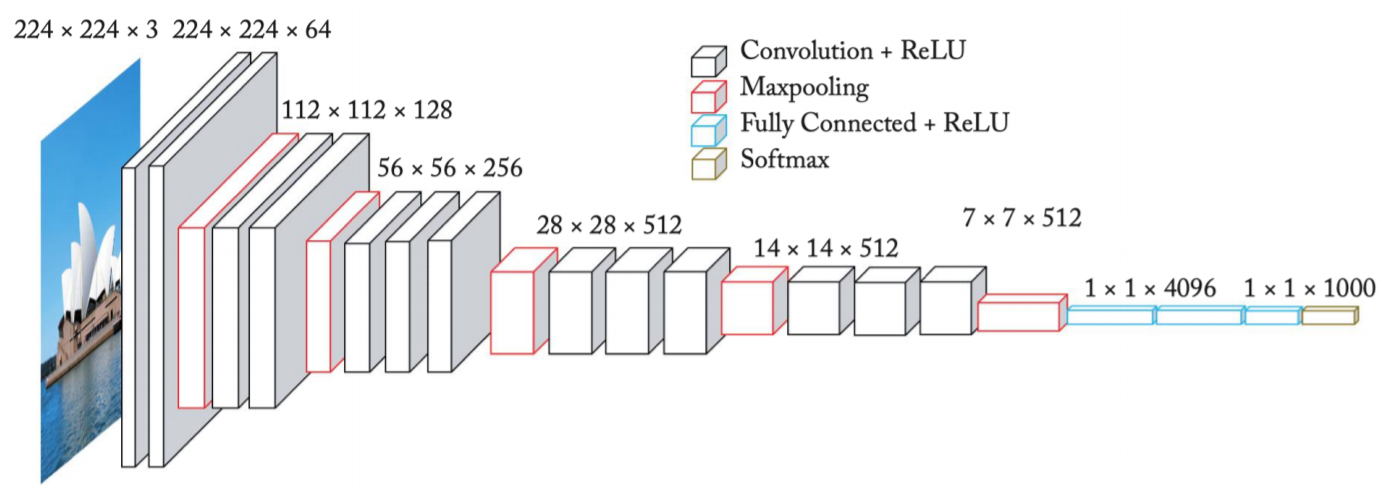
\includegraphics[width=0.8\textwidth]{../../imagens/ilustracoes/cap5_vgg16.png}
%   \par \textbf{Source: \cite{Cao:2020}, based on \cite{VGGNET:2014}.}
%   \label{fig:architecture_vgg16}
% \end{figure}

%The work developed here followed the approaches present in the networks  HED \cite{HED:2015} and RCF \cite{RCF:2017:8100105}, which make changes in the final layers to build their architectures.
To build our architecture, the last activation layer and all the fully connected layers of the VGG16 network were removed.
Also it was added side-outputs in different quantities, for evaluation.
In the first proposal, side-outputs were added in the last convolution of each stage, while in the second, secondary outputs were added after each convolutional layer.
Details regarding these architectures, influence on training and accuracy will be discussed in Sections \ref{cap5_saidas_laterais} and \ref{cap6_experm_1_qtd_saidas}.
An overview of the architecture can be seen in Figure \ref{fig:method}.

VGG16 was chosen due its overall performance and its relatively simplicity to create, train and study the influence of side-outputs, being suitable for our experiments. 
Creating, training and analyzing the influence of outputs is a simpler task than in residual networks such as ResNet \cite{RESNET:2016:7780459}, despite its higher performance.

%--------------------------------
%SUB - INFLUÊNCIA DO NÚMERO DE SAÍDAS laterais
\subsection{Side-outputs}
\label{cap5_saidas_laterais}

In addition to following the VGG16 architecture, the work used side-outputs, like several other existing approaches described in Section \ref{cap4_trab_rel}.
To evaluate the most appropriate number of side-outputs, it was analyzed HED and RCF architectures.
HED creates outputs after the last convolutional layer of each stage (5 outputs), while RCF adds side-outputs after each of the convolutions (13 outputs) \cite{HED:2015} \cite{RCF:2017:8100105}.

The first strategy, named \textit{Stage Layer Outputs} (\textbf{SLO}) and inspired by the HED model, creates a side-output $\mathcal{H}_i$ for each stage $S$ of the network.
Its graphical representation is available in Figure \ref{fig:architecture_slo}.
The second strategy, named \textit{All Layers Outputs} (\textbf{ALO}) and inspired by the RCF architecture, creates a side-output $\mathcal{H}_i$ for each convolutional layer $L$, as detailed in Figure \ref{fig:architecture_alo}.

\begin{figure*}
  \centering
  \caption{SLO Neural Network Architecture.}
  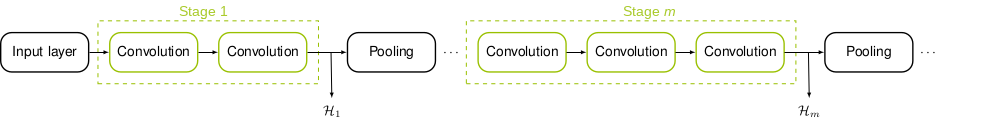
\includegraphics[width=0.7\textwidth]{../../imagens/ilustracoes/cap6_arquitetura_slo.png}
  \sourceOwn
  \label{fig:architecture_slo}
\end{figure*}

\begin{figure*}
  \centering
  \caption{ALO Neural Network Architecture.}
  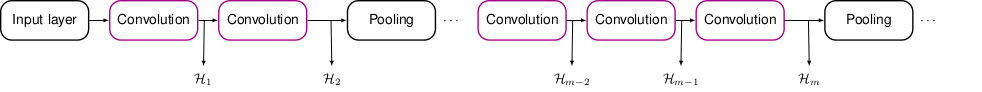
\includegraphics[width=0.7\textwidth]{../../imagens/ilustracoes/cap6_arquitetura_alo.png}
  \sourceOwn
  \label{fig:architecture_alo}
\end{figure*}

% \begin{figure}
%   \centering
%   \caption{SLO Neural Network Architecture.}
%   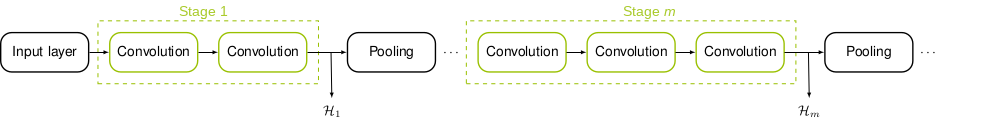
\includegraphics[width=1\columnwidth]{../../imagens/ilustracoes/cap6_arquitetura_slo.png}
%   \sourceOwn
%   \label{fig:architecture_slo}
% \end{figure}
% 
% \begin{figure}
%   \centering
%   \caption{ALO Neural Network Architecture.}
%   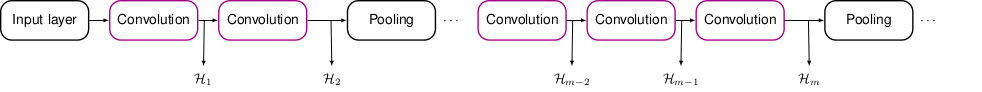
\includegraphics[width=1\columnwidth]{../../imagens/ilustracoes/cap6_arquitetura_alo.png}
%   \sourceOwn
%   \label{fig:architecture_alo}
% \end{figure}

In SLO, the number of side-outputs corresponds to the number of network stages $|S|$.
In turn, in the ALO method, the amount of output equals the number of convolutional layers $|L|$.
Formally, the set $ \mathcal{H}$ of $m$ side-outputs maps in each strategy is defined as:

\begin{align}
\mathcal{H}_{SLO}=\{\mathcal{H}_1,...,\mathcal{H}_m~|&~ m \le |S|\}\\
\mathcal{H}_{ALO}=\{\mathcal{H}_1,...,\mathcal{H}_m~|&~ m \le |L|\}
\end{align}

Each side-output $\mathcal{H}_1, ... \mathcal{H}_m$ is composed of a $1 \times 1$ convolution, followed by a transposed convolution of variable size.
Due to the network architecture, with \textit{pooling} layers, the images are reduced along the network. 
Thus, for the images to be resized to a single size, it is necessary that the transposed convolutions have a variable size.
%The evaluation of the learning curve and final post-training performance of each strategy will be presented in Section \ref{cap6_experm_1_qtd_saidas}.

%--------------------------------
%SUB - TÉCNICAS PARA COMBINAR SAÍDAS LATERAIS
\subsection{Side-outputs Merging Techniques}
\label{cap5_func_combinar_saidas}

Working with side-outputs requires that methods be used to combine intermediate results.
These are generated at different scales and may represent different concepts due to the position of the output on the network.
The goal, then, is to produce a single proposition $\hat{Y}$ to be evaluated in the task, keeping useful information contained in different layers.

In this work, a new strategy is developed to overcome the challenge of combining the outputs by exploring the knowledge of the learning process.
Operations are performed element-wise at each side-output.
To do this, the initial step is to resize the images generated at different stages of the network, so that they all have the same size.
Then, different trivial merge functions were studied and compared, once each of these has an expected behavior, as described below:

\begin{itemize}
  %\itemsep0.1cm
  \item \textit{ADD}: sums intermediate results, aiming to balance negative and positive weights;
  \item \textit{AVG}: calculates the average value of the outputs to create a proposal that represents learning at all levels;
  \item \textit{MAX}: returns the maximum value between the results, aiming to value the most confident outputs.
\end{itemize}

Formally, the combined output $\mathcal{Z}$ in each strategy can be defined as:

\begin{align}
  \mathcal{Z}_{ADD} &= \sum_{i=1}^{m}(\mathcal{H}_i)\\
  \mathcal{Z}_{AVG} &= \frac{\sum_{i=1}^{m}(\mathcal{H}_i)}{m}\\
  \mathcal{Z}_{MAX} &= \max_{1 \leq i \leq m} (\mathcal{H}_i)
\end{align} 

%--------------------------------
\subsection{Merged Output}
\label{cap5_saida_final_rede}

After combining the side-outputs as detailed in Section \ref{cap5_func_combinar_saidas}, a single final prediction $\hat{Y}$ is produced.
The value is obtained by executing a convolutional operation of $1 \times 1$ followed by a ReLU activation function.
The method overview is illustrated in Figure \ref{fig:method}.

\begin{figure*}
  \centering
  \caption{Overview of our method.}
  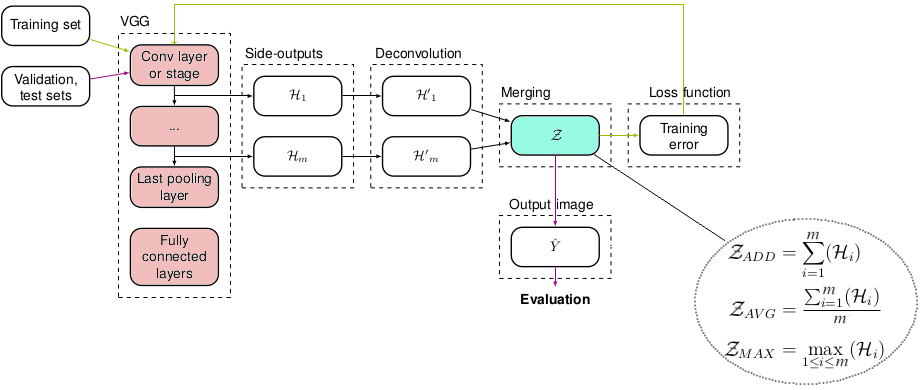
\includegraphics[width=0.7\textwidth]{../../imagens/ilustracoes/cap5_metodo.png}
  \sourceOwn
  \label{fig:method}
\end{figure*}

% \begin{figure}
%   \centering
%   \caption{Overview of our method.}
%   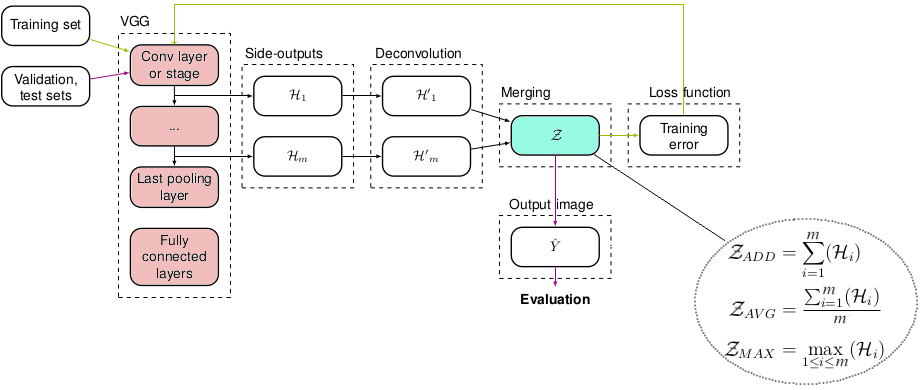
\includegraphics[width=1\columnwidth]{../../imagens/ilustracoes/cap5_metodo.png}
%   \sourceOwn
%   \label{fig:method}
% \end{figure}

In region segmentation tasks, $\hat{Y}$ seeks to provide partitions that represent significant areas of an image, while in the edge detection tasks, it seeks to represent the boundary between regions.

\begin{comment}
Na tarefa de segmentação multirregiões, a proposição $\hat{Y}$ pode ser reduzida a um problema binário.
Nele, objetivo seria distinguir cada pixel da imagem como pertencente a uma região de interesse ou ao fundo.
Se confrontado com múltiplas regiões de interesse, este mínimo de formulação pode ser executado individualmente e, os resultados, em seguida, unidos.
\end{comment}

%--------------------------------
\subsection{Class Balancing Methods}
\label{cap5_balanc_classes}

Edge detection seeks to identify abrupt change in an image aspect, like color or brightness \cite{MARTIN:1273918}.
In this problem, the number of edge pixels is considerably less than objects and background pixels.
Due to class imbalance, machine learning methods have difficult to identify edges.
Without proper treatment, the classification returns only backgound pixels, with high confidence.

To help to solve this problem, we decided to use Focal Loss, proposed by \cite{Lin:2017}, aims helps to solve problems with high imbalance between classes.
It is a change in Cross Entropy for binary classification function, that seeks to devalue pixels that are easy to identify and to value pixels that are hard to classify \cite{Lin:2017}.

% Consider the binary cross-entropy (CE) function, defined by Equation \ref{equ:cap6_cross_entropia1}, where $M$ is the number of training examples, $y_m$ is target label for a training example $m$ and $\hat{y}_m$ is the prediction of the neural network for a training example $m$ \cite{Ho:2019}.
% 
% \begin{equation}
%   CE = -\frac{1}{M} \sum_{m=1}^M [y_m \times log(\hat{y}_m) + (1 - y_m) \times log(1 - \hat{y}_m)]
%   \label{equ:cap6_cross_entropia1}
% \end{equation}
% 
% A weighted version of binary cross-entropy is given by a weight $\alpha$, generating Equation \ref{equ:cap6_cross_entropia2} \cite{Ho:2019}.
% 
% \begin{equation}
%   CE = -\frac{1}{M} \sum_{m=1}^M [\alpha \times y_m \times log(\hat{y}_m) + (1 - y_m) \times log(1 - \hat{y}_m)]
%   \label{equ:cap6_cross_entropia2}
% \end{equation}
% 
% To simplify the last equation, it is possible limits predictions $\hat{y} \in [0, 1]$ interval, and consider $p_t$ as the probability estimated for the class with label $y = 1$, as defined in Equation \ref{equ:cap6_cross_entropia3}, that can be rewritten in Equation \ref{equ:cap6_cross_entropia4}.
% 
% \begin{equation}
%    p = 
%   \begin{cases}
%     - \hat{y} & \quad \text{if } y = 1\\
%     - 1 - \hat{y} & \quad \text{otherwise }
%   \end{cases}
%   \label{equ:cap6_cross_entropia3}
% \end{equation}
% 
% \begin{equation}
%   CE = -\frac{1}{M} \sum_{m=1}^M [\alpha \times log(p_m)]
%   \label{equ:cap6_cross_entropia4}
% \end{equation}
% 
% Focal Loss proposes a modulation factor $(1 − p)^{\gamma}$, with a tunnable parameter $\gamma \ge 0$, that can smoothly adjusts the rate between easy and difficult samples \cite{Lin:2017}. It can be written as Equation \ref{equ:focal_loss}.
% 
% \begin{equation}
%   FL = - \frac{1}{M} \sum_{m=1}^M [(1 - p_m)^{\gamma} \times \alpha \times log(p_m)]
%   \label{equ:focal_loss}
% \end{equation}
% 
% % \begin{equation}
% %   FL(p_t) = - {\alpha_t} (1 - pt)^\gamma log(p_t), \quad \text{where } \gamma \geq 0
% %   \label{equ:focal_loss}
% % \end{equation}
% 
% % The $\alpha$ parameter seeks to balance the importance of positive and negative examples, while $\gamma$ aims to work with a performance tuning hyperparameter \cite{Lin:2017}.


%--------------------------------
\section{Organization of Experiments}
%--------------------------------

%--------------------------------
%SUB - BASES DE DADOS
\subsection{Data sets}
\label{cap5_bases_dados}

The methods present in this work were evaluated in the following data sets, widely used and cited by different works in the literature:

\begin{itemize}
 \item KITTI Road/Lane: part of the Karlsruhe Institute of Technology and Toyota Technological Institute project, it provides a set of images, and their respective human-annotated ground truths of the roads and lanes \cite{Fritsch2013ITSC}; %\footnote{~KITTI Road/Lane: \url{http://www.cvlibs.net/datasets/kitti/}}

 \item BSDS500: the \textit{Berkeley Segmentation Data Set and Benchmarks 500} contains a set of natural images and their human-annotated ground truths for image segmentation and edge detection research. \cite{amfm_pami2011}; %\footnote{~BSDS500: \url{https://www2.eecs.berkeley.edu/Research/Projects/CS/vision/grouping/resources.html}}
 
 %\item NYU Depth v2\footnote{NYUD-v2: \url{https://cs.nyu.edu/~silberman/datasets/}}: a base corresponde a um conjunto de imagens rotuladas de ambientes internos, obtidos por câmeras RGB e de profundidade do Microsoft Kinect. Contém também frames de sequências de vídeos não rotulados, que foram utilizados para gerar as imagens da base \cite{Silberman:ECCV12};
\end{itemize}
%--------------------------------

%--------------------------------
%SUB - FERRAMENTAS PARA AVALIAÇÃO
\subsection{Evaluation Tools and Benchmarking}
\label{cap5_formas_avaliacao}

The quality evaluation of the results were made using benchmarks of the own data sets. % or projects developed for this purpose.
The following benchmarks were used:

\begin{itemize}
 \item KITTI Road/Lane Evaluation: benchmark of the KITTI suite, estimates roads and tracks based on birds-eye-view space. It returns \textit{f-measure}, precision and recall values, false positive and false negative rates. \cite{Fritsch2013ITSC};
 
 \item BSDS500 Benchmark: BSDS500 benchmark for segmentation quality assessment. It uses precision and recall methods to classify results of segmentation and boundaries \cite{amfm_pami2011};
 
 %\item SEISM: acrônimo de \textit{Supervised Evaluation of Image Segmentation Methods}, permite a avaliação de métodos de segmentação usando técnicas de precisão e revocação em bordas, objetos e partes. \cite{Pont-Tuset2016a}.
\end{itemize}
%--------------------------------

%--------------------------------
%SUB - FERRAMENTAS E APIs
% \subsection{Development Tools and APIs}
% \label{cap5_ferramentas_api}
% 
% The Python programming language was used to develop the method and the experiments.
% The following frameworks, libraries and tools for neural network development, creation, comparison and validation of the methods were used:
% 
% \begin{itemize}
%   \item \textit{Tensorflow}\footnote{~Tensorflow: \url{https://www.tensorflow.org}}: open source platform for machine and deep learning, developed by the Google Brain Team \cite{tensorflow2015-whitepaper};
%  
%   \item \textit{Keras}\footnote{~Keras: \url{https://keras.io}}: high-level open-source neural networks API, running on top of Tensorflow \cite{chollet2015keras}.
%  
%   \item \textit{OpenCV}\footnote{~OpenCV: \url{http://opencv.org/}}: multiplatform library for application development in Computer Vision and Image Processing.
%  
%   \item \textit{Scikit-Learn}\footnote{~Scikit-Learn: \url{https://scikit-learn.org/stable/}}: open source machine learning library containing tools for mining and data analysis.
%  
%   \item \textit{SciPy}\footnote{~SciPy: \url{https://scipy.org/}}: Python library that provides a variety of functionality for math, science and engineering.
% \end{itemize}
%--------------------------------

%--------------------------------
%SUB - EXPERIMENTAL SETUP
\subsection{Experimental Setup}
\label{cap5_experimental_setup}

Our networks were built using using Keras \cite{chollet2015keras} with Tensorflow \cite{tensorflow2015-whitepaper}. 
We used a pre-trained VGG16 model to initialize the weights. 
Training experiments were performed in GeForce GTX 1080 8GB GPU\footnote{Some experiment were performed using a GeForce GTX 1660 6GB GPU}.
%--------------------------------

%--------------------------------
%SUB - EXPERIMENTAL SETUP
\subsection{Dataset Visualization}
\label{cap5_dataset_visualization}

{\color{red}

\cite{Vellido:2011}
\cite{Chatzimparmpas:2020}
\cite{Hohman:2019}
\cite{Chang:2016}

Lorem ipsum dolor sit amet, consectetur adipiscing elit. Aenean ornare risus nec est efficitur, sit amet lacinia risus vestibulum. Maecenas justo enim, fringilla non euismod pharetra, cursus eget sapien. Aenean feugiat pharetra justo. Sed commodo at nibh vitae dignissim. Ut porta, orci ut fringilla eleifend, diam orci fringilla dui, eget laoreet velit erat eu nisi. Praesent rhoncus sapien porttitor lobortis euismod. In vel diam nec lacus luctus rutrum. Etiam quis vulputate dolor. Sed non quam ac ligula vehicula volutpat non id sem. Phasellus orci nulla, posuere id ultricies non, ultrices ut nulla. Cras auctor ac nibh vel laoreet. Pellentesque maximus accumsan iaculis.

}

% \begin{figure}%[h!]
%   \centering
%   \caption{KITTI uu\_road colormap visualization.}
%   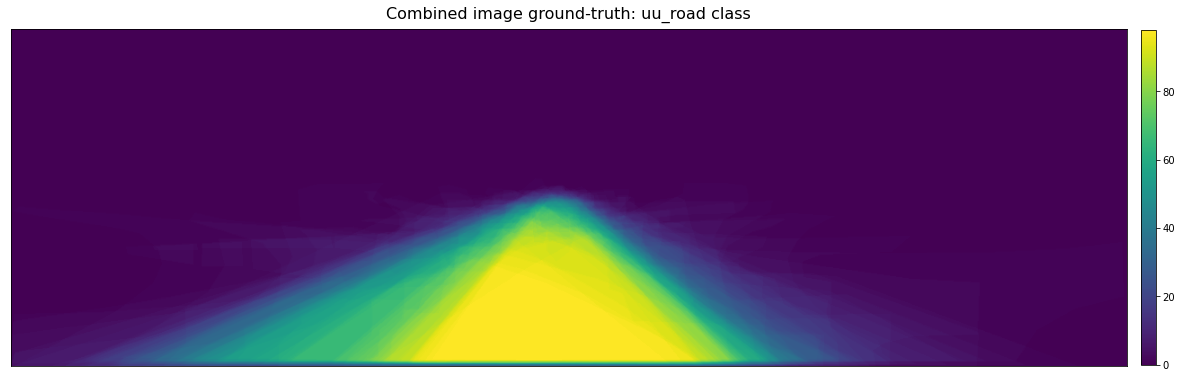
\includegraphics[width=1\columnwidth]{../imagens/visualiz_dados/kitti_uu_road_colormap.png}
%   \sourceOwn
%   \label{fig:kitti_uu_road_colormap}
% \end{figure}
% 
% \begin{figure}%[h!]
%   \centering
%   \caption{KITTI um\_road colormap visualization.}
%   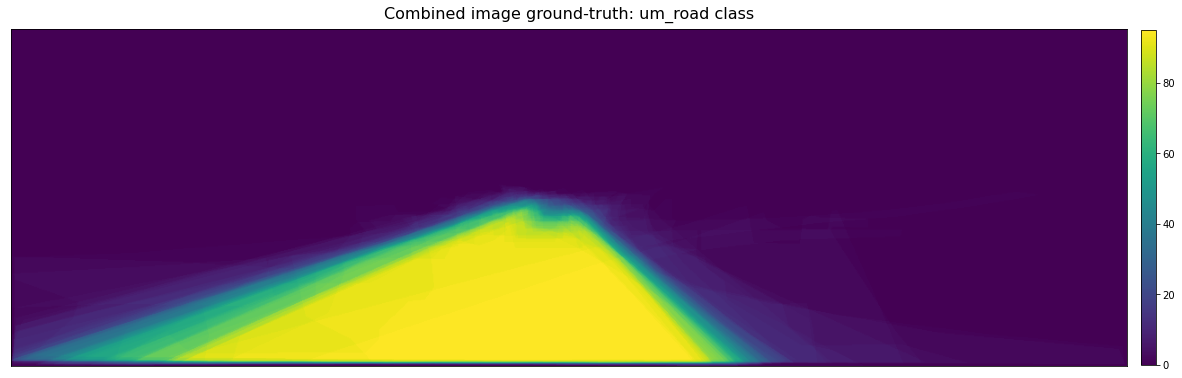
\includegraphics[width=1\columnwidth]{../imagens/visualiz_dados/kitti_um_road_colormap.png}
%   \sourceOwn
%   \label{fig:kitti_um_road_colormap}
% \end{figure}
% 
% \begin{figure}%[h!]
%   \centering
%   \caption{KITTI umm\_road colormap visualization.}
%   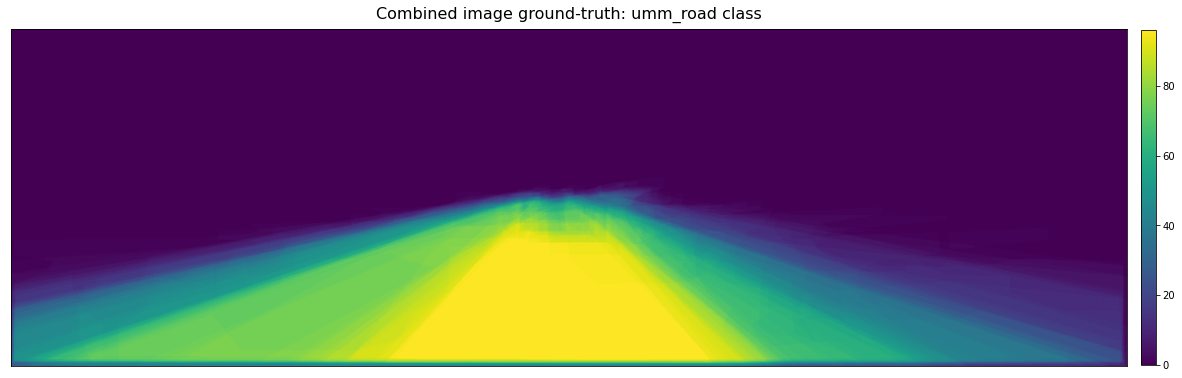
\includegraphics[width=1\columnwidth]{../imagens/visualiz_dados/kitti_umm_road_colormap.png}
%   \sourceOwn
%   \label{fig:kitti_umm_road_colormap}
% \end{figure}
% 
% \begin{figure}%[h!]
%   \centering
%   \caption{KITTI um\_lane colormap visualization.}
%   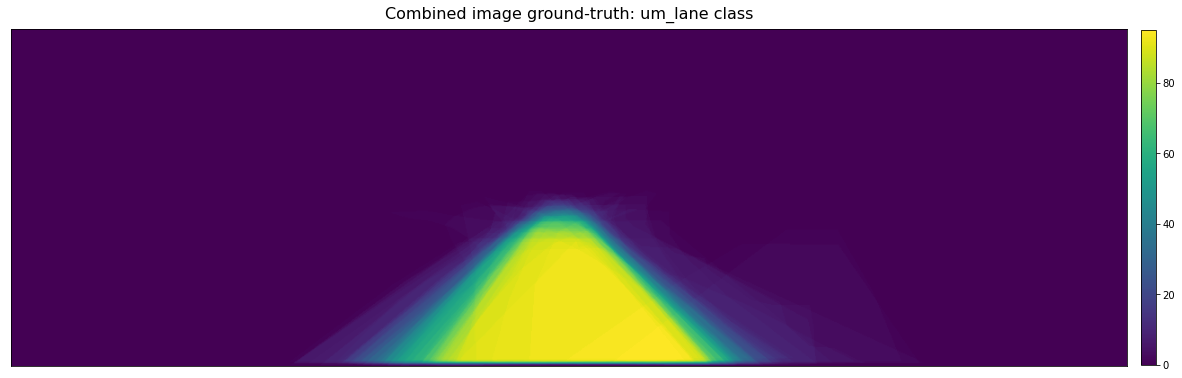
\includegraphics[width=1\columnwidth]{../imagens/visualiz_dados/kitti_um_lane_colormap.png}
%   \sourceOwn
%   \label{fig:kitti_um_lane_colormap}
% \end{figure}

%--------------------------------


%--------------------------------
%ORGANIZAÇÃO DOS EXPERIMENTOS
% \subsection{Organization of Experiments}
% \label{cap6_organiz_experimentos}
% 
% The experiments were organized as it follows:
% 
% \begin{enumerate}
%   \item \textit{Region Segmentation - KITTI Dataset} \\
%   The first experiment aimed to analyze the feasibility of the method described in Section \ref{cap5_metodologia}.
%   For an initial analysis, the region segmentation task was considered more appropriate, as it requires a lower level of precision than edge detection problems.
%   Also, it was evaluated the influence of the amount of side-outputs and the performance of the methods to combine them.
%   
%   \item \textit{Border Detection - BSDS500} \\  
%   The second experiment aimed to evaluate the method performance  in edge detection, a more complex and precise task than region segmentation.
%   BSDS500 was chosen due its small size, relative simplicity and its wide use in the literature, which makes it suitable for comparison to the literature.
% \end{enumerate}

%--------------------------------
%--------------------------------

%--------------------------------
%RESULTADOS
\section{Region Segmentation Experiments}
\label{cap6_result_experm_1}

The first set of experiments aimed to analyze the feasibility of the method described in Section \ref{cap5_metodologia}.
For an initial analysis, the region segmentation task was considered more appropriate, as it requires a lower level of precision than edge detection problems.
Also, it was evaluated the influence of the amount of side-outputs and the performance of the methods to combine them.

The experiments were conducted using the KITTI Road/Lane data set.
This data set is composed of 289 training and 290 test images with size of $1242 \times 375$ pixels. 
Ground truth is manually annotated for two different pixel types: $(i)$ \textbf{road} is the area of the road that makes up all lanes; and $(ii)$ \textbf{lane} is the ego-lane where the vehicle is currently in \cite{Fritsch2013ITSC}.

KITTI data set contains only ground truth for training data.
The test set is evaluated using the KITTI Server Evaluation.
In the work developed, only road markings were considered and images for lane segmentation were ignored.
The ground truth of roads is divided into three categories: $(i)$ urban unmarked (\textbf{uu\_road}), $(ii)$ urban marked (\textbf{um\_road}), $(iii)$ urban multiple marked lanes (\textbf{umm\_road}) \cite{Fritsch2013ITSC}.

To increase the number of images in the training set, data-augmentation techniques were used.
The following transformations have been applied: salt/pepper noise, noise shadow, horizontal inversion (mirroring), contrast and brightness change, random rain/snow addition.
Data augmentation procedures that create unwanted behavior, such as vertical inversion and distortions that would change the nature of objects in the scene, such as cars and pedestrians, have been avoided.
Enlargement procedures resulted in 2601 images, divided into 2080 training samples and 521 validation samples (about 20\%).

The initialization of weights was based on a pre-trained VGG16 model\footnote{VGG16 model was trained using ImageNet dataset \cite{ILSVRC15}.}.
In addition, we use Stochastic Gradient Descen (SGD) optimization with $1 \times 10^{-3}$ learning rate, $5 \times 10^{-6}$ learning decay and 0.95 momentum.
To tune the network and speed up the process, all images have been scaled down to $624 \times 192$ pixels (about 50\%). 
The default batch size had 16 images.

%--------------------------------
\subsection{Influence of merging methods and the number of side-outputs}
\label{cap6_experm_1_qtd_saidas}

The first test of the current experiment was designed to identify the influence of the number of side-outputs and the best merging methods.
For this, it were used \textbf{ALO} and \textbf{SLO} networks, detailed in Section \ref{cap5_saidas_laterais}.
The networks have been trained for only 100 epochs, using each merging methods.
It was also used a modified VGG16 version to predict regions, without side-outputs, as baseline, called in this work \textit{No Side-Outputs} (\textbf{NSO}).
%Figure \ref{fig:kitti_validation_loss_100epochs} shows the loss curves during the training phase for the validation set.

% \begin{figure}
%   \centering
%   \caption{Validation loss using \textit{Categorical Cross Entropy} metric.}
%   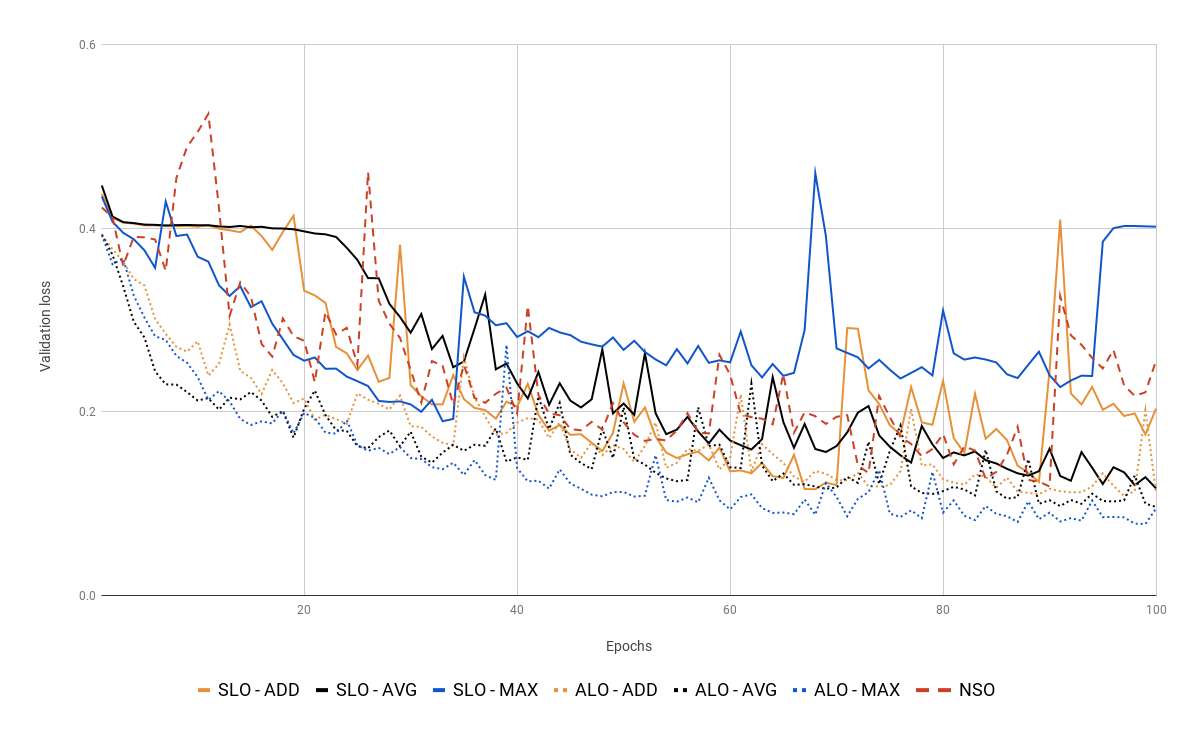
\includegraphics[width=1.\columnwidth]{../../imagens/graficos/cap6_kitti_validation_loss.png}
%   \sourceOwn
%   \label{fig:kitti_validation_loss_100epochs}
% \end{figure}

It is observed in the first part of the experiment that the ALO networks appear to be more stable, with a steeper loss curve than the NSO and all SLO approaches.
% In addition, it is important to note that the NSO and SLO-MAX networks are highly unstable during learning phase, with abrupt changes in the loss value, resulting in graphical spikes.
In addition, NSO and SLO-MAX networks were highly unstable during learning phase, with abrupt changes in the loss value, resulting in graphical spikes.
On the other hand, the ALO-AVG network had the best result, followed by ALO-MAX and ALO-ADD.
This is possibly caused by the considerably higher number of outputs, which creates the possibility of exchange between confident values.

To improve results, a new round of testing was created with 500 training epochs.
As SLO networks showed poor performance in the previous test and other tests performed with different parameters, then it was decided to evaluate only ALO networks.
The network NSO was also trained as a comparison \textit{baseline}.

Performance analysis was done by two different metrics: the well-known \textit{Categorical Cross Entropy} and \textit{Pixel-error} metric.
Pixel-error was adopted when high precision values were observed in results where there were noticeably many errors, especially with numerous false positives.
% The performance of the above networks using both metrics is shown in Figures \ref{fig:kitti_cross_entropy_500_epochs} and \ref{fig:kitti_pixel_error_500_epochs}. 
%It can be observed that side-outputs have a positive influence on the performance of the networks.
All versions of network ALO outperforms NSO network using both metrics.

% \begin{figure}
%   \centering
%   \caption{Performance of ALO and NSO nets using \textit{Categorical Cross Entropy} metric.}
%   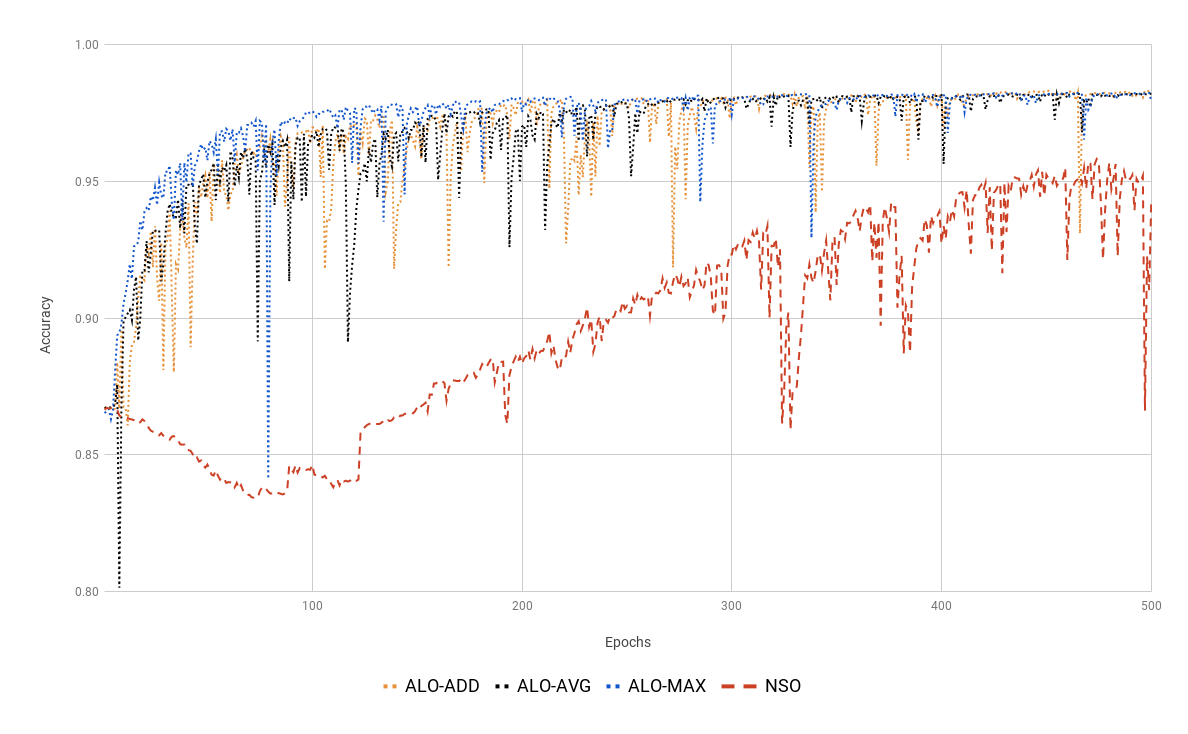
\includegraphics[width=1.\columnwidth]{../../imagens/graficos/cap6_kitti_val_acc_500_epochs.png}
%   \sourceOwn
%   \label{fig:kitti_cross_entropy_500_epochs}
% \end{figure}
% 
% \begin{figure}
%   \centering
%   \caption{Performance of ALO and NSO nets using \textit{Pixel-Error} metric.}
%   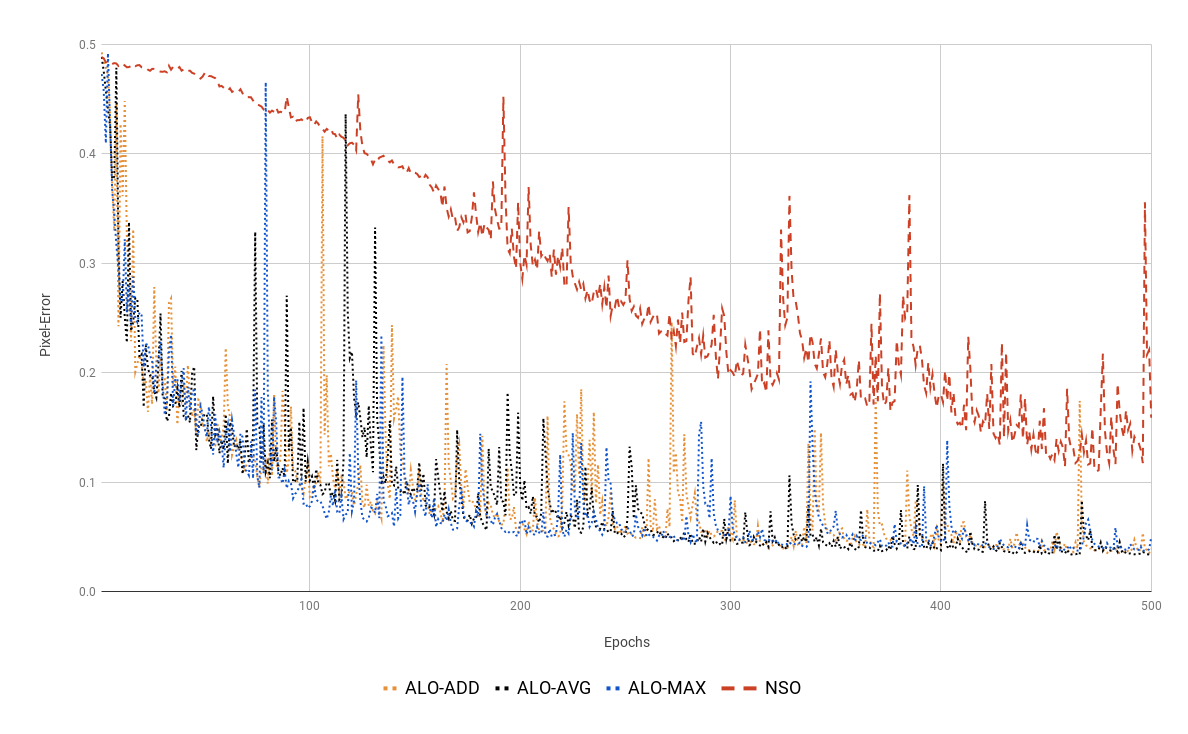
\includegraphics[width=1.\columnwidth]{../../imagens/graficos/cap6_kitti_pixel_error_500_epochs.png}
%   \sourceOwn
%   \label{fig:kitti_pixel_error_500_epochs}
% \end{figure}

The results of the merging techniques of the ALO networks have similar value, indicating the absence of a considerably superior method to the others.
The best result for \textit{Categorical Cross Entropy} metric slightly outperforms the worst method (0.983 for ALO-ADD and 0.9821 for ALO-AVG).
Using \textit{Pixel-error metric}, the best value is only 0.004 higher than the worst (0.0332 for ALO-AVG and 0.0372 for ALO-MAX).

%--------------------------------
%SUB - CONTRIBUIÇÕES SAÍDAS laterais
\subsection{Side-Outputs Contribution}
\label{cap6_contribuicoes_saidas_intermediarias}

The layers in each merging strategy learn uniquely.
The contributions to the final prediction differ according to the merging method adopted, as shown in Figure \ref{fig:kitti_side_outputs}.
To make the analysis of the image clearer, only last side-output maps of each stage were plotted.
In addition, the images were transformed into monochromatic (binary), with white pixels representing the road and black pixels representing the background.

% \begin{figure*}
%   \centering
%   \caption{Side-output maps for ALO network merging strategies in KITTI Road/Lane data set.}
%   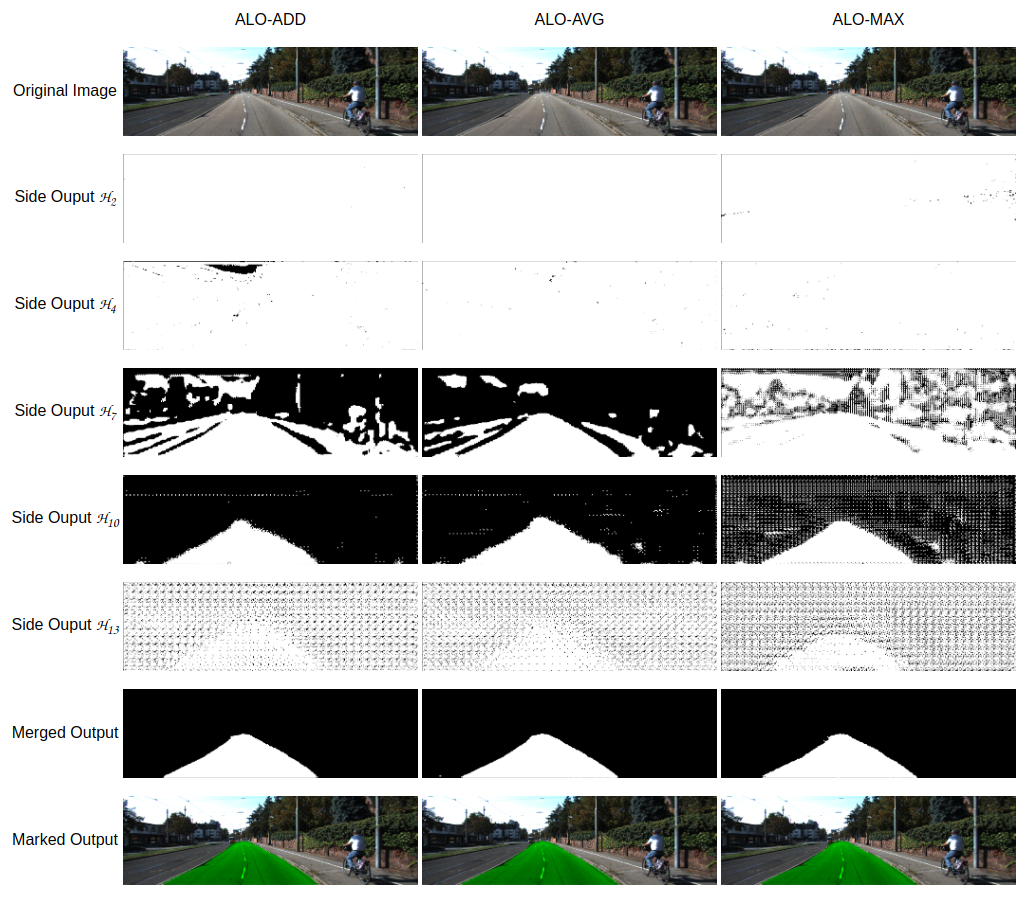
\includegraphics[width=0.7\textwidth]{../../imagens/ilustracoes/cap6_kitti_side_outputs.png}
%   \sourceOwn
%   \label{fig:kitti_side_outputs}
% \end{figure*}

\begin{figure}
  \centering
  \caption{Side-output maps for ALO network merging strategies in KITTI Road/Lane data set.}
  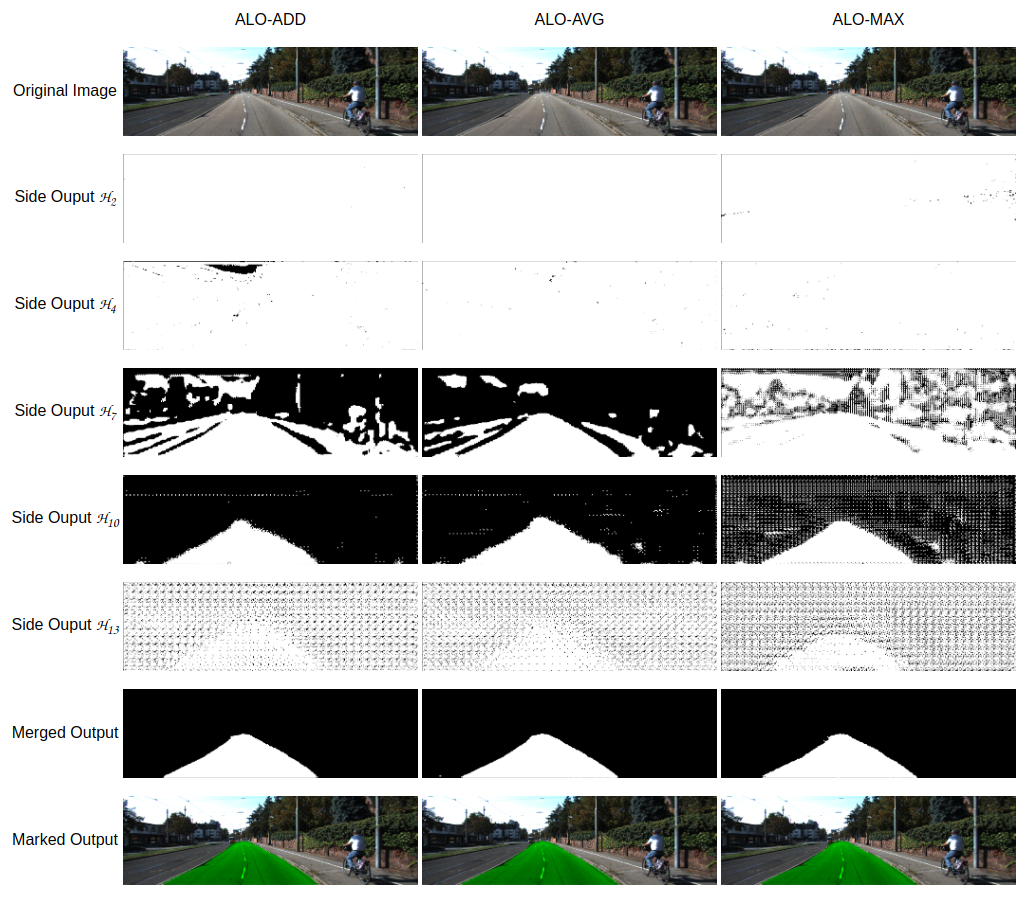
\includegraphics[width=1\columnwidth]{../../imagens/ilustracoes/cap6_kitti_side_outputs.png}
  \sourceOwn
  \label{fig:kitti_side_outputs}
\end{figure}

It can be seen from Figure \ref{fig:kitti_side_outputs} that the first two stages ($\mathcal{H}_2$ and $\mathcal{H}_4$) side-outputs does not produce meaningful information.
The images have mostly white pixels, indicating classification of all pixels as road.
In the third stage (output $\mathcal{H}_7$), the merging methods ALO-AVG and ALO-ADD, contains a obvious separation between road pixels and the background.
The output map $\mathcal{H}_7$, using ALO-MAX method, however, does not clearly separate road from non-road pixels.

Figure \ref{fig:kitti_side_outputs} further shows that the best side-output maps for all networks ALO are generated in the fourth stage $\mathcal{H}_{10}$. 
Road markings are visible even if there are noises, especially in the ALO-MAX method.
The final side-output, $\mathcal{H}_{13}$, contains high noise level.
This feature indicates that the layer was not able to learn correctly.

The merged output combines all side-outputs, including other intermediate results not available in Figure \ref{fig:kitti_side_outputs}, for prediction.
Despite the poor results in some layers, the learning process adjusts itself so that even bad results can be used by the model.

%--------------------------------
%PÓS PROCESSAMENTO
\subsection{Post Processing}
\label{cap6_pos_processamento}

At the end of the segmentation, a post processing step was added to reduce some noise.
For this, the \textit{morphological opening} operation was used to remove small noises created by the foreground (road) in the background.
The operation was applied using a $13 \times 13$ square structuring element as a result of empirical tests.

% A simple comparison of the final result with the original prediction is presented in Figure \ref{fig:kitti_post_processing_comp}.
% The image shows an example of benefit from the post processing step.
% It's possible to see the noise removal mainly at the right edge of the image (\textit{white pixels}).
% A side effect is the removal of some points that seem to fit properly, mostly in lower left and lower right corners of the road (\textit{red pixels}).
% 
% \begin{figure}%[h!]
%   \centering
%   \caption{Differences between original method results and after post processing.}
%   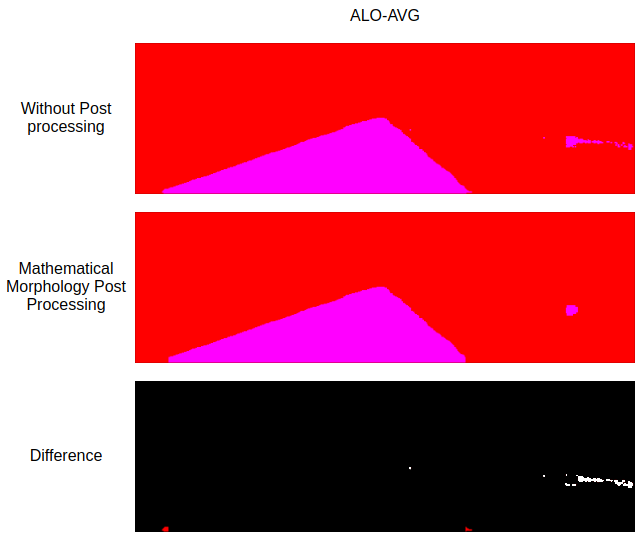
\includegraphics[width=0.9\columnwidth]{../../imagens/ilustracoes/cap6_kitti_post_proc_comp.png}
%   \sourceOwn
%   \label{fig:kitti_post_processing_comp}
% \end{figure}

%--------------------------------
%SUB - RESULTADOS DA SEGMENTAÇÃO
\subsection{Segmentation Evaluation}
\label{cap6_resultados_segmentacao}

After the post-processing step, segmentation quality was evaluated.
The tests were performed using the ALO-AVG method, the best in the training phase.
Results were sent to  the KITTI Evaluation Server, with name of \textbf{ALO-AVG-MM}\footnote{~Results are available in a public leaderboard at \url{http://www.cvlibs.net/datasets/kitti/eval_road.php}}.
The server returned the following metrics: MaxF, AP, PRE, REC, FPR and FNR, whose results for each road scene category\footnote{~\textit{URBAN\_ROAD} category corresponds to the combination of the other three categories.}, as described in Section \ref{cap6_result_experm_1}, are available in Table \ref{tab:kitti_metrics}.

%table kitti_metrics
\begin{table}
  \centering
  \scriptsize
  \setlength{\tabcolsep}{0.8em}
  \renewcommand{\arraystretch}{1.7}
  \begin{tabular}{{l}{c}{c}{c}{c}{c}{c}}
    \hline
    \textit{Benchmark} & MaxF & AP & PRE & REC & FPR & FNR
    \\
    \hline
    UM\_ROAD & 91.15\% & 83.82\% & 89.07\% & 93.33\% & 5.22\% & 6.67\%
    \\
    UMM\_ROAD & 94.05\% & 90.96\% & 94.82\% & 93.29\% & 5.60\% & 6.71\%
    \\
    UU\_ROAD & 89.45\% & 79.87\% & 85.40\% & 93.90\% & 5.23\% & 6.10\%
    \\
    \hline
    URBAN\_ROAD & 92.03\% & 85.64\% & 90.65\% & 93.45\% & 5.31\% & 6.55\%
    \\
    \hline
  \end{tabular}
  \caption{Segmentation performance on KITTI Road Dataset.}
  \label{tab:kitti_metrics}
\end{table}


%The results available in Table \ref{tab:kitti_metrics} show how efficient the method is.
Compared to the best result on the KITTI platform named PLARD \cite{Chen:2019}\footnote{~At the time of our first conference paper submission, \cite{Reis:2019}, \textit{PLARD} had not yet been published in the literature, being an anonymous submission on KITTI platform.}, our method had an overall performance 5.0\% lower.
It is also necessary to remember that the model was trained for only 500 epochs.
Thus, it is indicated that the techniques for combining side-outputs had good results, as desired.

To show the performance of our model, Figure \ref{fig:kitti_representacao_visual} was created with ALO-AVG-MM predictions\footnote{~More visual results are public available on \href{http://www.cvlibs.net/datasets/kitti/eval_road_detail.php?result=a5ca173550cb383caf3e12ca236d7c809489d2d9}{KITTI Server}.}.
Pixels have been labeled as true positives (\textit{green}), false negatives (\textit{red}) and false positives (\textit{blue}).
The original images were created by the KITTI Evaluation Server, based on the binary map sent to the server.

%\begin{sidewaysfigure}
\begin{figure}
  \centering
  \caption{Visual representation of ALO-AVG-MM predictions}
  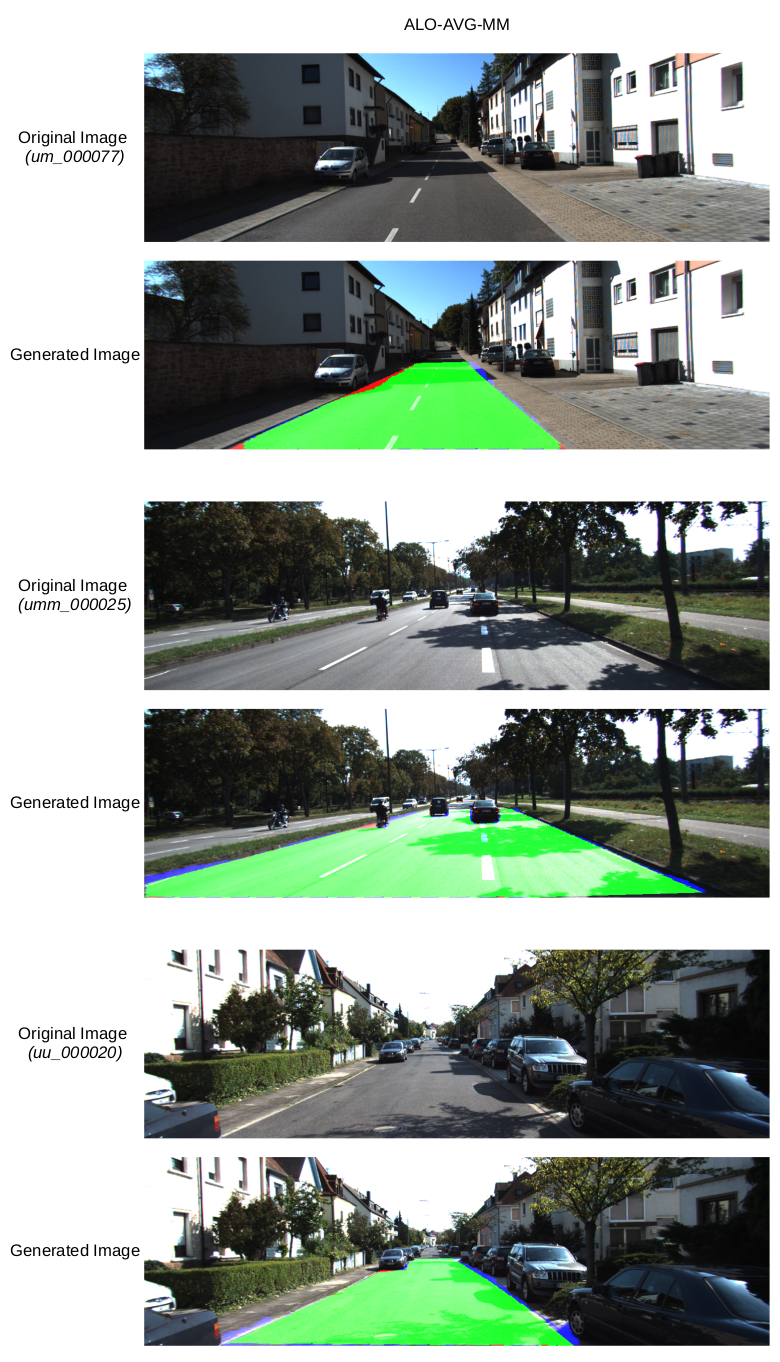
\includegraphics[width=0.9\columnwidth]{../../imagens/ilustracoes/cap6_kitti_visual_representation.png}
  \sourceOwn
  \label{fig:kitti_representacao_visual}
\end{figure}
%\end{sidewaysfigure}
%--------------------------------

%--------------------------------
\section{Border Detection Experiments}
\label{cap6_result_experm_2}

The second set of experiments aimed to evaluate the method performance  in edge detection, a more complex and precise task than region segmentation.
BSDS500 was chosen due its small size, relative simplicity and its wide use in the literature, which makes it suitable for comparison to the literature.

BSDS500 consists in a set of 500 images with size of $480 \times 320$ pixels\footnote{~For boundary detection, images contains a extra pixel ($481 \times 321$ or $321 \times 481$)}.
The set is explicit subdivided into training, validation and test, containing 200, 100 and 200 images, respectively.
Ground truths are manually annotated by five different subjects on average. 
It contains ground truth for region segmentation and border detection \cite{amfm_pami2011}.

{\color{blue}
To visualize the data set and understand better the problem, Figure \ref{fig:bsds_colormap} was developed.
Unlike the KITTI database, the BSDS database does not contain pixels of interest distributed in a specific position of the image, making training difficult.
Thus, it becomes necessary to use methods that can work with unbalanced classes, as discussed in the Section \ref{cap5_balanc_classes}.
}

\begin{figure}%[h!]
  \centering
  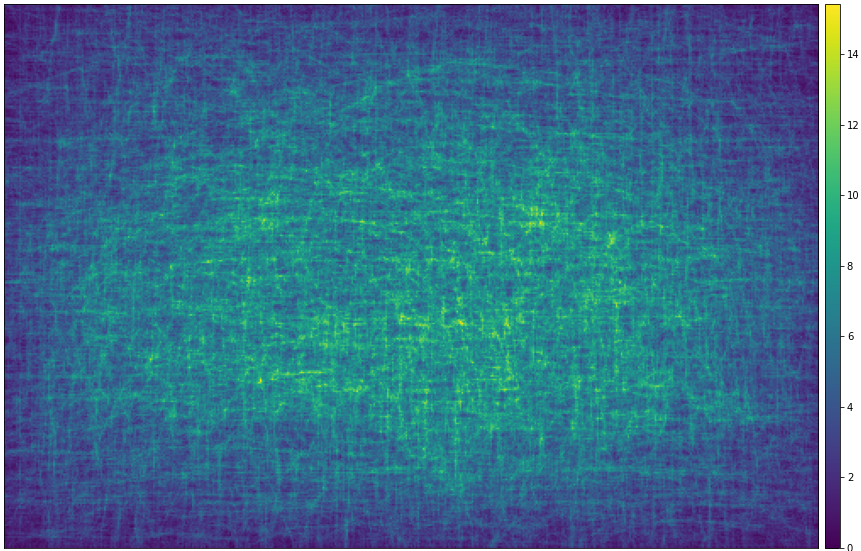
\includegraphics[width=1\columnwidth]{../imagens/visualiz_dados/bsds_colormap.png}
  \caption{BSDS500 combined ground truth colormap.}
  \label{fig:bsds_colormap}
\end{figure}

BSDS500's test set is evaluated using BSDS500 Benchmark, provided by the authors \cite{amfm_pami2011}.
In our experiments, training and validation sets were merged into one group, in order to increase generalization.
The test set was only used to evaluate the performance of our results.

To increase training performance, it was used some data augmentation techniques, as salt and pepper noise, log and gamma contrast, JPEG compression, dropout, affine and perspective transformations, crop, pad, among others.
Rotation, flipping, mirroring and zoom (with factors of 0.5, 1.0 and 1.5) were combined with the techniques previously described.
All procedures resulted in 11400 images (38 samples per image).%\footnote{Code to generate these images are publicly available at \url{https://github.com/falreis/alo-seg-edge}}.
%The network was trained using 9690 images and validate on 1710 samples.
%Rotation procedure used the reflection technique to avoid cutting, empty regions or image size changing.

As previous experiments, the ground truth was separated into two binary classes, corresponding to the background and the edges.
However, after training, the system was changed to maintain classes, but to generate results based on confidence, in the range of 0 to 1, and no longer in binary form.
This method allows the identification of soft borders, as will be explained in the Section \ref{ssec:groundtruth_analysis}.%, and the definition of a border threshold, as \citeonline{Cumulative:Song20181847} paper.

Of all the experiments carried out, only a few important ones were detailed in this next subsections.
The analysis of experiments are summarized in Section \ref{cap6_discussion}.
%Other network architectures and test variations are available in Appendix \ref{apend:a}.

%--------------------------------
\subsection{Ground truth analysis}
\label{ssec:groundtruth_analysis}

As briefly reported previously, BSDS500's ground truths are manually annotated by five different subjects on average \cite{amfm_pami2011}.
Due multiples ground truths, some experiments were conducted to define how to combine them, in order to help the network to learn properly.
To do that, we developed 3 different methods to combine them.

The first ground truth representation, named \textbf{ALL}, added all ground truths and divided them by the maximum of ground truths' overlaps in each image.
Ground truths borders were represented in a interval of 0 to 1, where the \textit{1-value} represents borders annotated in all ground truths, while the \textit{0-value} represents background in every annotation.
Values in between, correspond to soft borders, annotations marked in one or more ground truths but not in all them.
This representation is shown in Figure \ref{sfig:cap6_bsds_100075_all}.

\begin{figure*}%[h!]
  \centering
  \subfloat[\label{sfig:cap6_bsds_100075_orig_all}]{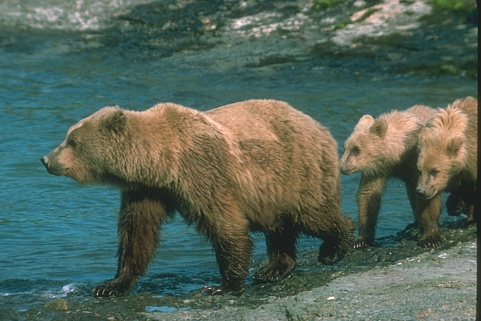
\includegraphics[width=0.24\textwidth]{../imagens/ilustracoes/cap6_bsds_100075.jpg}}
  \hfill
  \subfloat[\label{sfig:cap6_bsds_100075_all}]{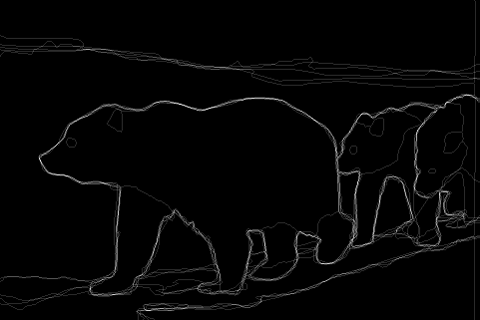
\includegraphics[width=0.24\textwidth]{../imagens/ilustracoes/cap6_bsds_100075_all.png}}
  \hfill
  \subfloat[\label{sfig:cap6_bsds_100075_upper}]{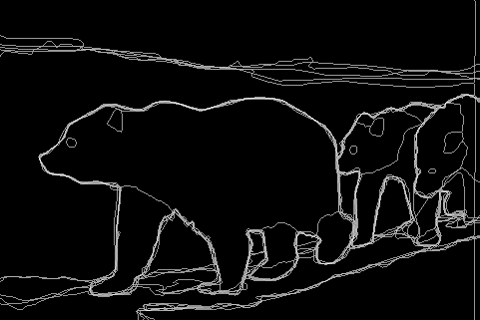
\includegraphics[width=0.24\textwidth]{../imagens/ilustracoes/cap6_bsds_100075_upper.png}}
  \hfill
  \subfloat[\label{sfig:cap6_bsds_100075_morf}]{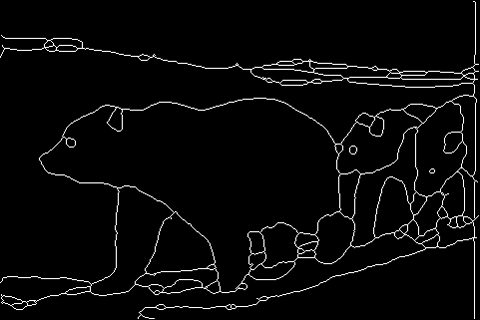
\includegraphics[width=0.24\textwidth]{../imagens/ilustracoes/cap6_bsds_100075_morf.png}}
  \caption{(a) BSDS500 image and its ground truth, using (b) ALL, (c) UPPER and (d) MORPH representations.}
  \label{fig:cap6_bsds_all}
\end{figure*}

This method had two major problems:

\begin{enumerate}
    \item As the number of ground truths for an image increases, some borders has really small values, almost close to the background value;
    \item Some borders are really close to others, but they do not overlap. So, the ground truth shows two different boundaries, which can make training difficult.
\end{enumerate}

One possible solution to fix the first problem is to limit boundaries to the interval of 0.5 to 1.0.
Background pixels are defined with value zero.
Once this method limited border in the upper range of values, it was named \textbf{UPPER}.
This ground truth representation method is available in Figure \ref{sfig:cap6_bsds_100075_upper}.

% \begin{figure}
%   \centering
%   \subfloat[\label{sfig:cap6_bsds_100075_orig_upper}]{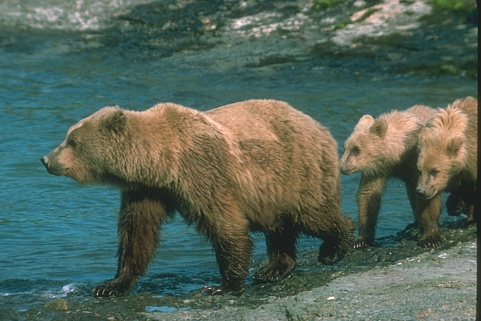
\includegraphics[width=0.48\textwidth]{../imagens/ilustracoes/cap6_bsds_100075.jpg}}
%   \hfill
%   \subfloat[\label{sfig:cap6_bsds_100075_upper}]{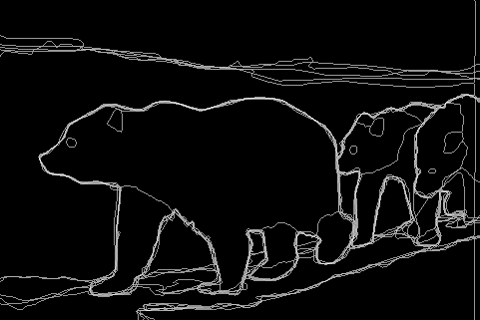
\includegraphics[width=0.48\textwidth]{../imagens/ilustracoes/cap6_bsds_100075_upper.png}}
%   \label{fig:cap6_bsds_upper}
%   \caption{(a) BSDS500 image and (b) its ground truth, using UPPER representation.}
% \end{figure}

Although benefits of the first approach, the second problem is not solved by them.
To settle it, an morphological set of operations were proposed to join close borders.
The chosen method corresponds to the dilatation of the boundaries using a kernel of $3 \times 3$, followed by a morphological thinning.
Dilation helps to join borders, but produced some shadows, that are removed by morphological thinning.

However, once morphological thinning is a binary operation, this method removes difference of values between borders, transforming soft borders into "hard borders", with values equal 1. 
The visual result of the morphological operations, named \textbf{MORPH}, is available in Figure \ref{sfig:cap6_bsds_100075_morf}.

% \begin{figure}
%   \centering
%   \subfloat[\label{sfig:cap6_bsds_100075_orig_morf}]{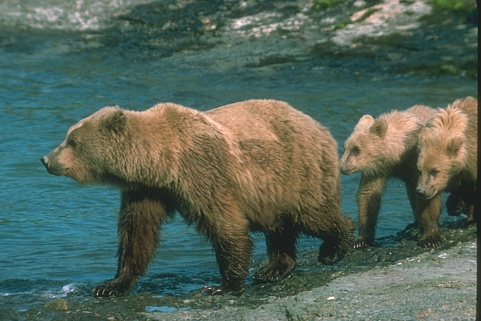
\includegraphics[width=0.48\textwidth]{../imagens/ilustracoes/cap6_bsds_100075.jpg}}
%   \hfill
%   \subfloat[\label{sfig:cap6_bsds_100075_morf}]{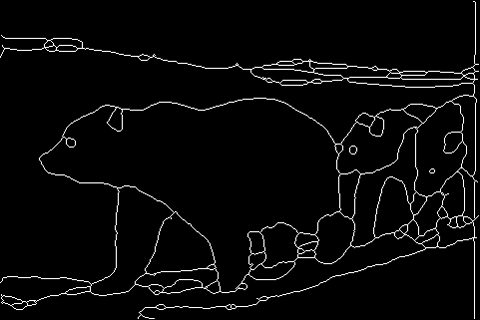
\includegraphics[width=0.48\textwidth]{../imagens/ilustracoes/cap6_bsds_100075_morf.png}}
%   \label{fig:cap6_bsds_morf}
%   \caption{(a) BSDS500 image and (b) its ground truth, using MORPH representation.}
% \end{figure}

Some initial experiments were performed to evaluate the three approaches.
It was observed that training the network using only ALL ground truth resulted into poor performance, due difficult of generalization.
The best generalization for early stage training was produced using MORPH ground truths.
However, ALL and UPPER ones, applied after a some MORPH training, produced better visual results.

%--------------------------------
\subsection{Protocol for experiments}
\label{ssec:framework_experiments}

%This section will describe the protocol developed for training our networks. 
As described in Section \ref{ssec:groundtruth_analysis}, the use of ground truth \textit{MORPH} in the early stages of training achieved the best generalization.
After it, the usage of \textit{ALL} and \textit{UPPER} ground truths improves achieved results.
For this, we developed the following protocol, with the following phases:

\begin{enumerate}
    \item Train only deconvolutional layers with MORPH ground truth;
    \item Train the whole network with MORPH ground truth;
    \item Train the whole network using ALL or UPPER ground truths;
\end{enumerate}

The first step starts with pre-trained VGG16 model.
The results produced by first training phase, in terms of loss value, will be used by the following step.
Likewise, the second step produces the weights for third training phase.
At the end, the weights produced in the last phase are used to evaluate the network performance.

The following parameters set as standard in our experiments with BSDS500, unless otherwise specified:
\begin{itemize}
    \item Learning method: SGD
    \item Activation: ReLU
    \item Learning rate: $1 \times 10^{-6}$ (first step) and $1 \times 10^{-7}$ (others)
    \item Learn. decay: $1 \times 10^{-10}$ (first step) and $1 \times 10^{-11}$ (others)
    \item Batch size: 8 images
    \item Merging method: ALO
    \item Loss: Focal Loss ($\gamma$=2.0; $\alpha$=0.25)\footnote{~Parameters recomended by \cite{Lin:2017} paper.}
    \item Initial weights: VGG-16
    \item Training samples: 9690 images 
    \item Validation samples: 1710 images
    \item Image size: $384 \times 288$
\end{itemize}

In addition to the parameters listed previously, it was decided to use some functions to automatically reduce the learning rate and finish the training procedure after a number of epochs without any improvements. 
Learning rate (LR) is reduced by factor of 0.3 ($LR \times 0.3$), after 10 epochs, if the loss does not decrease, in absolute value, at least 0.5 units.

After loss decreasing, the code waits for 5 epochs (\textit{cooldown}) and the procedure repeats until the learning rate achieves $1 \times 10^{-9}$, when it stops decreasing.
Concomitantly with learning rate reduction, the early stopping procedure finishes training when the absolute value does not decrease at least 0.5 units after 50 epochs.
If early stopping is not reached, the code will be completed after 1000 training epochs.

%--------------------------------
\subsection{Experiment 2.1 - Basic experiment}
\label{ssec:bsds_subexp1}

To assess the network's performance, training was carried out with each version of the ALO network.
The training presented here follows the protocol and parameterization described in Section \ref{ssec:framework_experiments}.

The current experiment will be described into four subsections.
The first three ones will describe each network behavior in phases using MORPH ground truth.
The last section will compare final training results.

%--------------------------------
\subsubsection{ALO-ADD}
\label{ssec:bsds_subexp1_add}

The first network trained in the protocol was the ALO-ADD, which proved to be more stable in different preliminary tests.
The network quickly converged from pre-trained weights and after about 130 epochs, it has stabilized, with small performance gains.
After no gain for 50 epochs, the protocol ended its first phase.
%The training and validation losses from phases 1 and 2 in the protocol are shown in Figure \ref{fig:bsds_add_focal_morf_v1v2}.

% \begin{figure}%[h!]
%   \centering
%   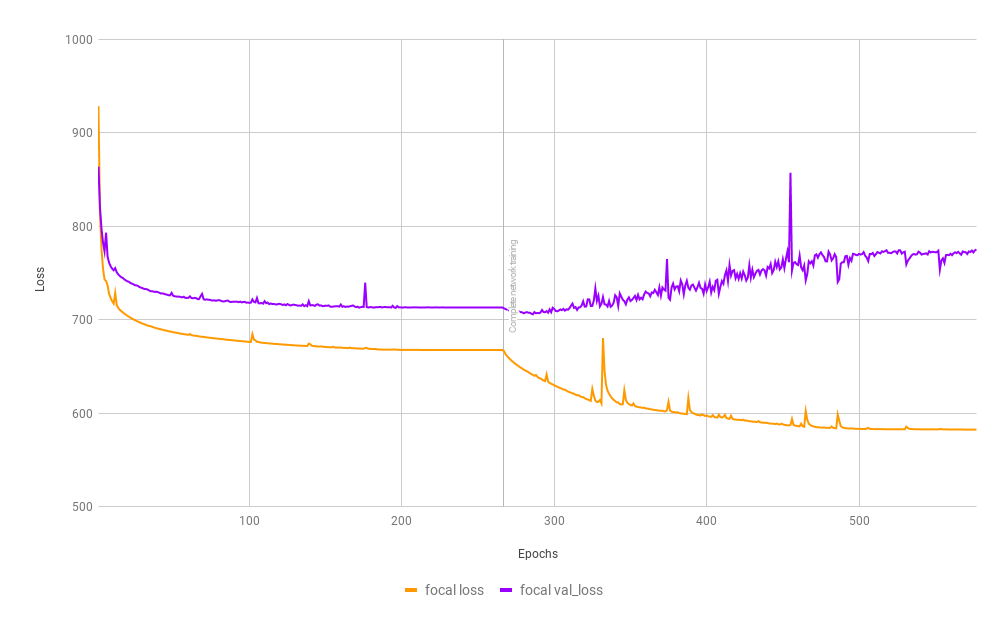
\includegraphics[width=1.\columnwidth]{../imagens/graficos/cap6_bsds_add_focal_morf_v1v2_20200409.png}
%   \caption{Training and validation losses using ALO-ADD/MORPH method on BSDS500.}
%   \label{fig:bsds_add_focal_morf_v1v2}
% \end{figure}

% It can be seen, that the network quickly converged from pre-trained weights.
% After about 130 epochs, the network has stabilized, with small performance gains.
% After no gain for 50 epochs, the protocol ended its first phase.

In second phase of the protocol, the network had a sharp decay in the training loss. %, as can be seen in Figure \ref{fig:bsds_add_focal_morf_v1v2}.
Contrarily, validation loss increased (this condition will be carefully analysed in Section \ref{ssec:basic_pred_eval}).
Close to the 500th epoch, the network showed again poor training loss decrease and it was finished in the 567th epoch.

%--------------------------------
\subsubsection{ALO-AVG}
\label{ssec:bsds_subexp1_avg}

The second network trained in the protocol was the ALO-AVG, which had similar performance to ALO-ADD in preliminary tests.
ALO-AVG promptly converged, with a behavior similar to ALO-ADD.
After around 140 epochs, the network has stabilized, with small performance gains. 
The protocol has ended its first phase (only deconvolutions training) at the epoch 219.
%The training and validation losses from steps 1 and 2 of the protocol are shown in Figure \ref{fig:bsds_avg_focal_morf_v1v2}.

% \begin{figure}%[h!]
%   \centering
%   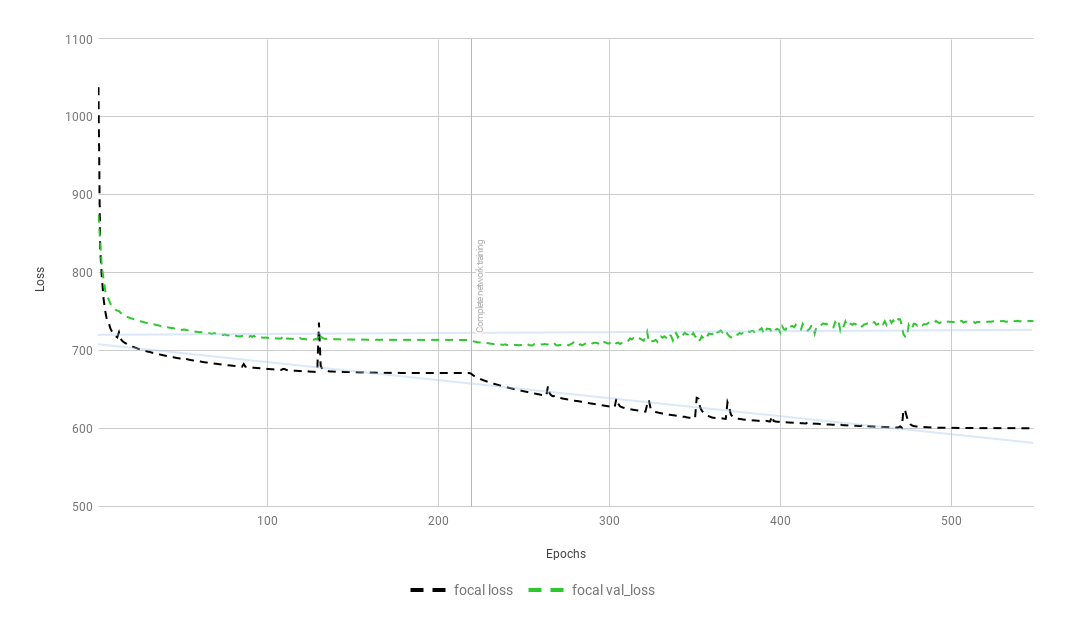
\includegraphics[width=1.\columnwidth]{../imagens/graficos/cap6_bsds_avg_focal_morf_v1v2_20200407.png}
%   \caption{Training and validation losses using ALO-AVG/MORPH method on BSDS500.}
%   \label{fig:bsds_avg_focal_morf_v1v2}
% \end{figure}

% It can be seen in Figure \ref{fig:bsds_avg_focal_morf_v1v2}, that the ALO-AVG promptly converged, with a behavior similar to ALO-ADD.
% After around 140 epochs, the network has stabilized, with small performance gains. 
% The protocol has ended its first phase (only deconvolutions training) at the epoch 219.

In the second phase, the training loss began to decrease slowly, but the validation loss increased, also slowly, for most of the process.
This increase is similar to the training of ALO-ADD, even if it is less than that presented in the previous experiment.
It is important to note that this behavior occurred even with small learning rates (less than $1 \times 10^{-9}$). 

%--------------------------------
\subsubsection{ALO-MAX}
\label{ssec:bsds_subexp1_max}

ALO-MAX was the last network trained in this experiment.
Contrarily to other networks, ALO-MAX had more difficult to converge properly in preliminary tests.
It had the lowest loss (722.39), 24.06\% more when compared to ALO-ADD (582.29) and 20.29\% more when compared with ALO-AVG (600.54).
%The training and validation losses of ALO-MAX's protocol in phases 1 and 2, the are presented in Figure \ref{fig:bsds_max_focal_morf_v1v2}.

%It can be seen in Figure \ref{fig:bsds_max_focal_morf_v1v2} that the ALO-MAX converged less and slower than the other networks.
%ALO-MAX had the lowest loss (722.39), 24.06\% more when compared to ALO-ADD (582.29) and 20.29\% more when compared with ALO-AVG (600.54).

% \begin{figure}%[h!]
%   \centering
%   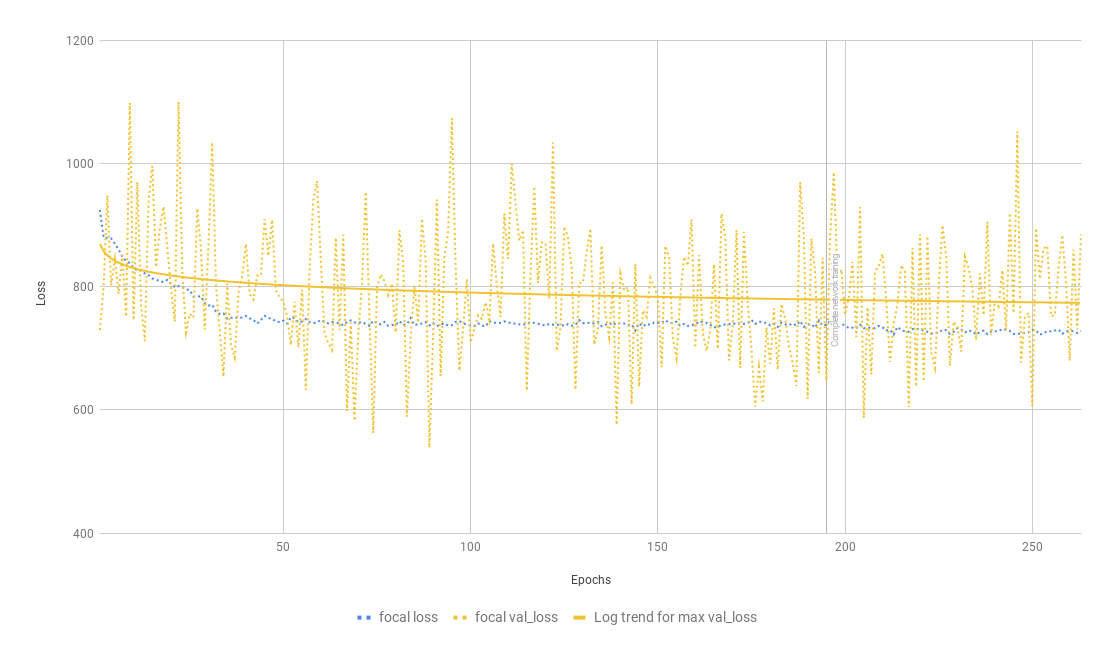
\includegraphics[width=1.\columnwidth]{../imagens/graficos/cap6_bsds_max_focal_morf_v1v2_20200408.png}
%   \caption{Training and validation losses using ALO-MAX/MORPH method on BSDS500.}
%   \label{fig:bsds_max_focal_morf_v1v2}
% \end{figure}

It is also possible to notice that the validation loss was really unstable during both phases, with many ups and downs, without any convergence in the process.
The training was faster than the previous ones, with 94 epochs in the first phase and only 69 epochs in second one.

The second phase indicates that the network was almost training and did not improved its results.
It is possible to conclude that only the training of the deconvolution layers was enough for the network to reach the best possible value.

%--------------------------------
% \subsubsection{Networks comparison}
% \label{ssec:bsds_subexp1_comparison}
% 
% To assist in the evaluation of the third phase of the experiments, Figures \ref{fig:bsds_addavgmax_focal_all} and \ref{fig:bsds_addavgmax_focal_upper} with the loss curves were created.
% To aid comparison, the values are presented in a single image, even though the number of training epochs are different for each method.
% Figure \ref{fig:bsds_addavgmax_focal_all} shows training and validation curves for ALL ground truth while Figure \ref{fig:bsds_addavgmax_focal_upper} shows the results for UPPER's.
% 
% \begin{figure}%[h!]
%   \centering
%   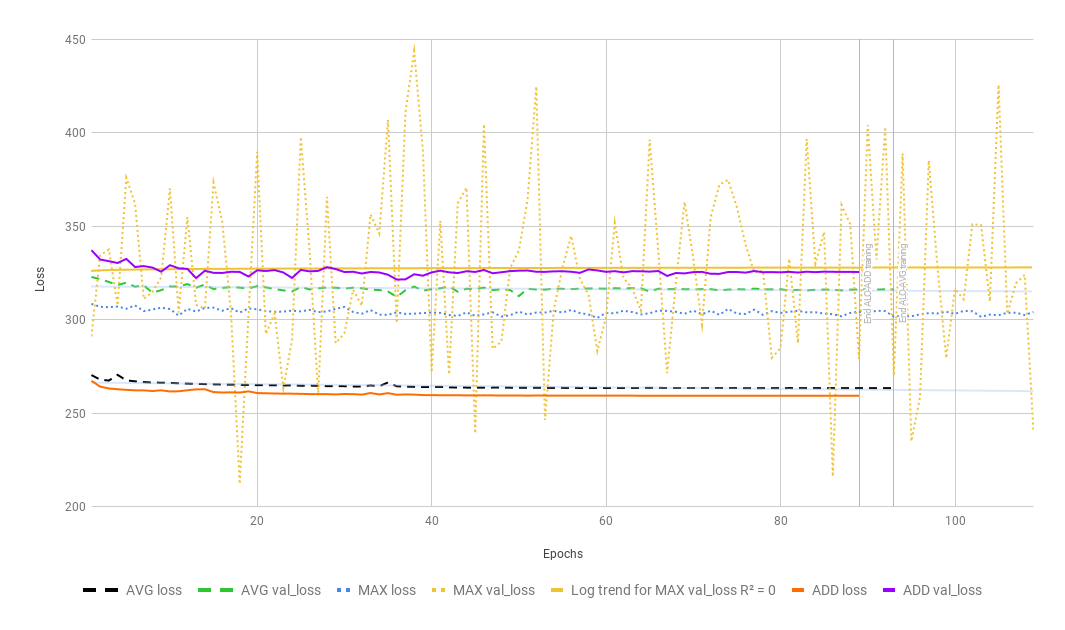
\includegraphics[width=1.\columnwidth]{../imagens/graficos/bsds_addavgmax_focal_all.png}
%   \caption{Loss comparison using ALL ground truth on BSDS500.}
%   \label{fig:bsds_addavgmax_focal_all}
% \end{figure}
% 
% \begin{figure}%[h!]
%   \centering
%   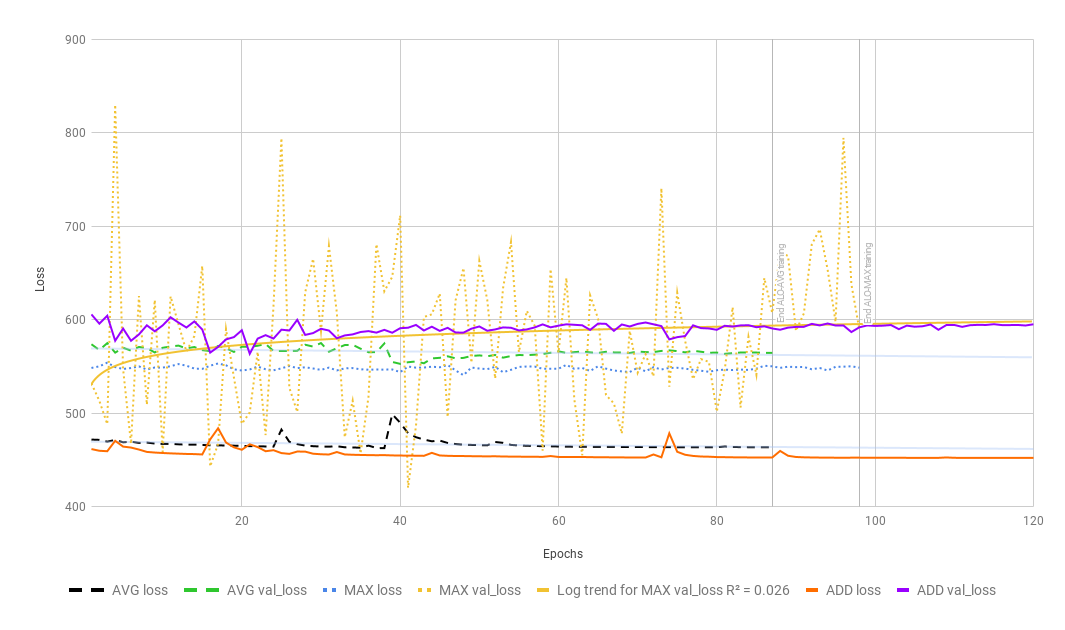
\includegraphics[width=1.\columnwidth]{../imagens/graficos/bsds_addavgmax_focal_upper.png}
%   \caption{Loss comparison using UPPER ground truth on BSDS500.}
%   \label{fig:bsds_addavgmax_focal_upper}
% \end{figure}
% 
% Figure \ref{fig:bsds_addavgmax_focal_all} shows predominantly a small training loss decrease during the entire procedure for the networks.
% In Figure \ref{fig:bsds_addavgmax_focal_upper}, it is possible to observe a higher nominal value of the loss when compared with Figure \ref{fig:bsds_addavgmax_focal_all}, caused by the different ground truth.
% The validation curves for ALO-ADD and ALO-AVG are somewhat unstable at the beginning of the process and becomes more stable throughout the training.
% 
% Figures \ref{fig:bsds_addavgmax_focal_all} and \ref{fig:bsds_addavgmax_focal_upper} shows that ALO-AVG and ALO-ADD had low fluctuation during all training period, without converging to smaller values.
% The gain were really small, indicating that networks are almost training.
% ALO-ADD training loss is smaller than ALO-AVG, but its validation loss was bigger during all training process.
% 
% It is possible to see in Figures \ref{fig:bsds_addavgmax_focal_all} and \ref{fig:bsds_addavgmax_focal_upper} that ALO-MAX presented the same problems as previously described in Section \ref{ssec:bsds_subexp1_max}.
% Validation loss kept unstable with high volatility, in opposite to its training loss.
% Despite the stability, the training loss had high value, making it closer to validation curves from AVG and ADD methods.
% This behavior indicates that the network was not able to generalize well. %, as can be seen in the performance analysis below.

% To complement the information provided by the analysis of losses, a performance evaluation was done using another metric, accuracy, as shown in Figure \ref{fig:bsds_focal_upper_metrics}.
% In there, it can be seen that training accuracy values are closes to 0.96 while validation accuracy is close to 0.9575, indicating that the data augmentation is sufficient for the problem and is also suitable for larger network architectures
% 
% \begin{figure}%[h!]
%   \centering
%   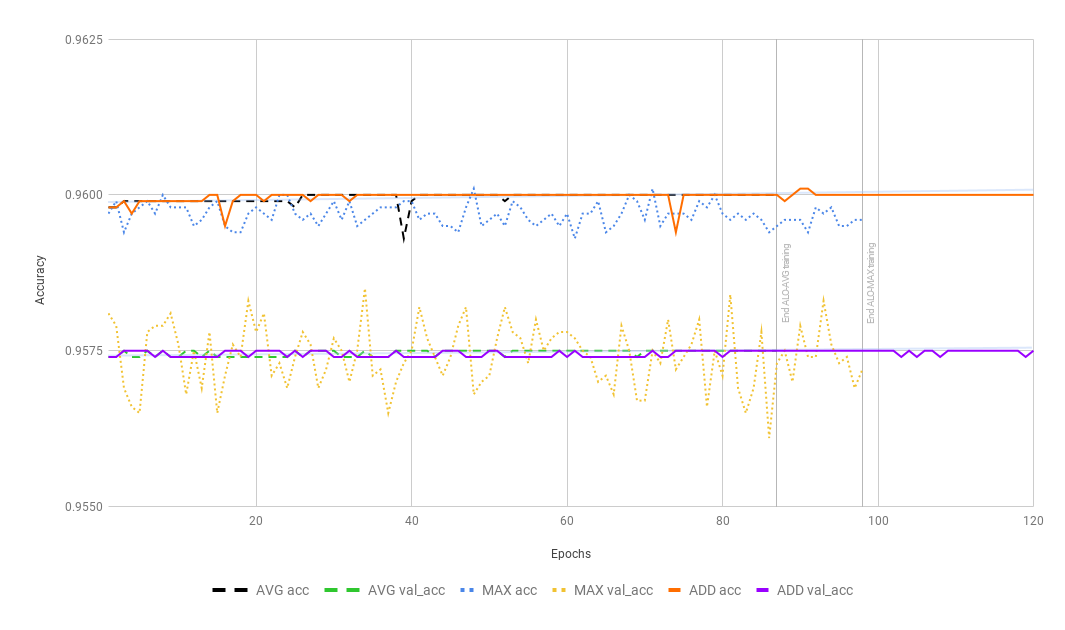
\includegraphics[width=1.\columnwidth]{../imagens/graficos/bsds_focal_upper_metrics.png}
%   \caption{Accuracy comparison using UPPER ground truth on BSDS500.}
%   \label{fig:bsds_focal_upper_metrics}
% \end{figure}
% 
% Figure \ref{fig:bsds_focal_upper_metrics} also indicates that ALO-MAX had close values to other methods, despite low performance in loss metrics.
% This can be explained due the number of background pixels in the image, making accuracy an inappropriate metric to evaluate the results.

\begin{comment}
Once the objective functions are different, it's not possible to compare metrics values returned by training statistics in each phase. 
For this, it was evaluated the results of border detection using BSDS500 Benchmark.
The results will be shown in Section \ref{ssec:basic_pred_eval}, when they will be compared to the results obtained by the ALO-AVG and ALO-MAX networks, that will be described in the following sections.
\end{comment}

%--------------------------------
\subsection{Evaluation and Predictions}
\label{ssec:basic_pred_eval}

Due to the low capacity to evaluate the previous experiments using the accuracy metric, it was decided to evaluate the model with BSDS500 Benchmark.
The results are presented in Figure \ref{fig:bsds_subexp1_results}. %Table \ref{tab:bsds_subexp1_results}.
To evaluate the gain of UPPER and ALL ground truths usage, it was decided to evaluate MORPH performance also.
As explained in Section \ref{ssec:framework_experiments}, the network was trained until it does not improve for 50 epochs, making MORPH almost unable to perform better.

% \begin{table}%[h!]
%   \centering
%   \caption{Border detection performance on BSDS500 for ALO-AVG, ALO-ADD and ALO-MAX.}
%   \scriptsize
%   \setlength{\tabcolsep}{1em}
%   \renewcommand{\arraystretch}{1.5}
%   \begin{tabular}{{c}{c}{c}{c}{c}{c}{c}}
%     \hline
%     Network & Loss & Ground truth & TH & ODS & OIS %& Area PR
%     \\
%     \hline
%     ALO-ADD & FL & MORPH (v1) & 0.51 & 0.7214 & 0.7461 %& 0.4721
%     \\
%     ALO-ADD & FL & MORPH (v2) & 0.50 & 0.7376 & 0.7596 %& 0.5331
%     \\
%     ALO-ADD & FL & ALL & 0.40 & 0.7504 & \textbf{0.7714} %& 0.6105
%     \\
%     ALO-ADD & FL & UPPER & 0.47 & \textbf{0.7512} & 0.7704 %& 0.5809
%     \\
%     ALO-AVG & FL & MORPH (v1) & 0.52 & 0.7227 & 0.7462 %& 0.4862
%     \\
%     ALO-AVG & FL & MORPH (v2) & 0.51 & 0.7384 & 0.7606 %& 0.5356
%     \\
%     ALO-AVG & FL & ALL & 0.40 & 0.7496 & 0.7708 %& 0.5932
%     \\
%     ALO-AVG & FL & UPPER & 0.46 & 0.7500 & 0.7690 %& 0.5796
%     \\
%     \hline
%     ALO-MAX & FL & MORPH (v1) & 0.70 & 0.6911 & 0.7127 %& 0.5712
%     \\
%     ALO-MAX & FL & MORPH (v2) & 0.67 & 0.7039 & 0.7247 %& 0.5510
%     \\
%     ALO-MAX & FL & ALL & 0.56 & 0.7122 & 0.7311 %& \textbf{0.6337}
%     \\
%     ALO-MAX & FL & UPPER & 0.64 & 0.7127 & 0.7326 %& 0.5932
%     \\
%     \hline
%   \end{tabular}
%   \label{tab:bsds_subexp1_results}
% \end{table}

\begin{figure*}%[h!]
  \centering
  %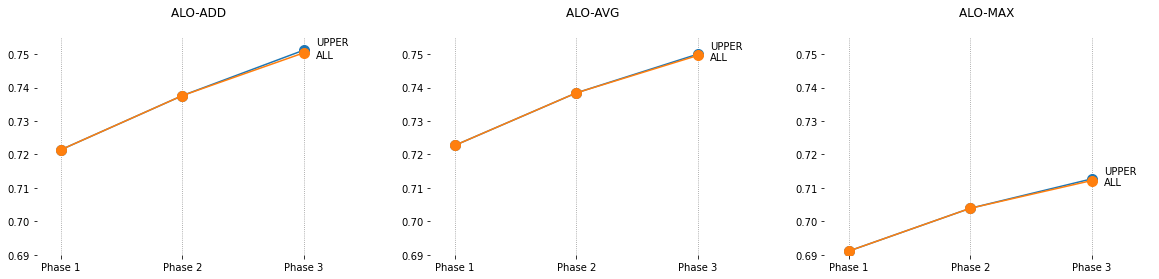
\includegraphics[width=0.8\textwidth]{../imagens/visualiz_dados/bsds_experiment_2-1.png}
  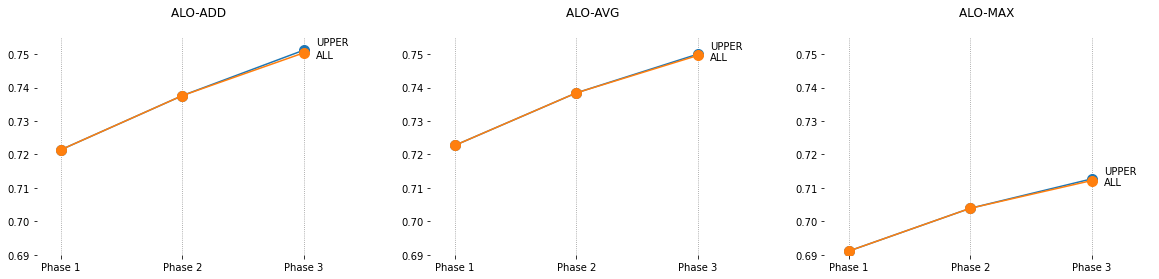
\includegraphics[width=1\textwidth]{../imagens/visualiz_dados/bsds_experiment_2-1.png} %VISUALIZ
  \caption{Border detection ODS performance on BSDS500 for ALO-AVG, ALO-ADD and ALO-MAX.}
  \label{fig:bsds_subexp1_results}
\end{figure*}

{\color{blue}
Figure \ref{fig:bsds_subexp1_results} was developed using small multiples technique to show the difference between methods.
ALO-ADD and ALO-AVG were plotted in different images once the results were similar and one data was above other.
This results contrasts with the poor performance of ALO-MAX network.
}

%It is possible to notice, in the analysis of Table \ref{tab:bsds_subexp1_results}, that all networks improved with training using ALL or UPPER ground truths.
It is possible to notice, in the analysis of Figure \ref{fig:bsds_subexp1_results}, that all networks improved with training using ALL or UPPER ground truths.
The benefit of using both ground truths is around 1,5\% in comparison with the best result achieved by MORPH ground truth.


% Using the analysis of Figures \ref{fig:bsds_addavgmax_focal_all} and \ref{fig:bsds_addavgmax_focal_upper}, it is important to remember that these networks have barely improved their performance in the last phase of the protocol.

These results can be partially explained due to the deformation caused by the morphological thinning operation.
UPPER and ALL ground truths maintains the original outline of the edges.
Also, the differences can be seen as just an adjust of the weights, to provide hard and soft defined borders.
This difference seens to influence the evaluation, once the benchmark compare borders with each human annotation in each ground truth.

\begin{comment}
It is also important to notice in Table \ref{tab:bsds_subexp1_results} that ALL and UPPER ground truths reduced the thresholds for the OIS and ODS values.
Once the threshold it is smaller than 0.5, this mean, in a binary way, that some borders are most similar to the background than the border class.
These borders just was plotted in the image because the values were presented in a scale of confidence, ignoring the most probable class.
When the MORPH ground truth was used, all classes were above 0.5, indicating that the results were well defined, despite the lower final result than those obtained with other ground truths.
\end{comment}

The overall results of ALO-ADD and ALO-AVG were really similar, but ALO-ADD had better performance using both ODS and OIS metrics.
The number of training epochs to reach the best results were also similar, as described in Table \ref{tab:bsds_subexp1_epochs}, but with less epochs for ALO-AVG.
These results indicates that both methods are similar in performance and number of training epochs.
Table \ref{tab:bsds_subexp1_epochs} also shows that ALO-MAX had the least number of training epochs.
However, due to its poor performance, this information cannot be used in favor of the method.

\begin{table}%[h!]
  \centering
  \caption{Number of training epochs using Focal Loss.}
  \scriptsize
  \setlength{\tabcolsep}{1em}
  \renewcommand{\arraystretch}{1.5}
  \begin{tabular}{{c}{c}{c}{c}{c}{c}{c}}
    \hline
    Ground truth & ALO-ADD & ALO-AVG & ALO-MAX
    \\
    \hline
    MORPH / ALL & 666 & 641 & 372
    \\
    MORPH / UPPER & 697 & 635 & 361
    \\
    \hline
  \end{tabular}
  \vspace{0.2cm}
  \label{tab:bsds_subexp1_epochs}
\end{table}

%To complete the information about training, it is important to view the visual results of the methods.
%These results are available in Figure \ref{fig:cap6_expr1_bsds_visual}, with the original prediction and with the best threshold cut, informed by the BSDS500 benchmark.

% \begin{figure*}
%   \centering
%   \captionsetup[subfigure]{labelformat=empty}
%   \subfloat[BSDS500 image\label{fig:cap6_expr1_img}]{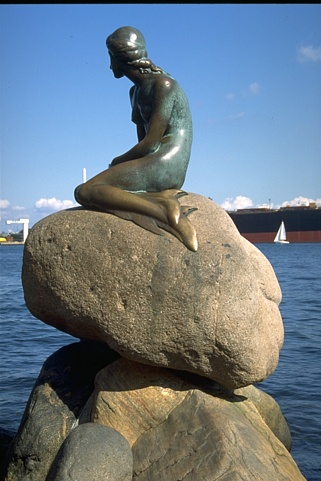
\includegraphics[width=0.24\textwidth]{../imagens/ilustracoes/cap6_bsds_372019.jpg}}
%   \hfill
%   \subfloat[ALO-ADD\label{fig:cap6_expr1_add}]{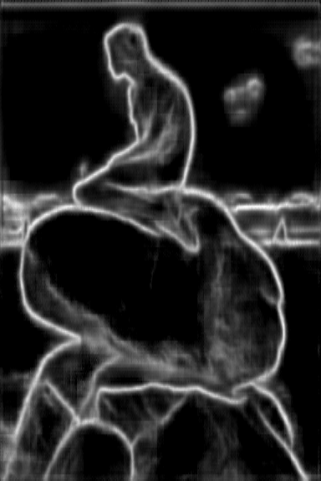
\includegraphics[width=0.24\textwidth]{../imagens/ilustracoes/cap6_bsds_372019_add_20200409.png}}
%   \hfill
%   \subfloat[ALO-AVG\label{fig:cap6_expr1_avg}]{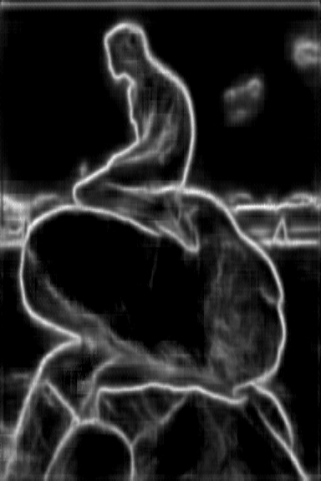
\includegraphics[width=0.24\textwidth]{../imagens/ilustracoes/cap6_bsds_372019_avg_20200407.png}}
%   \hfill
%   \subfloat[ALO-MAX\label{fig:cap6_expr1_max}]{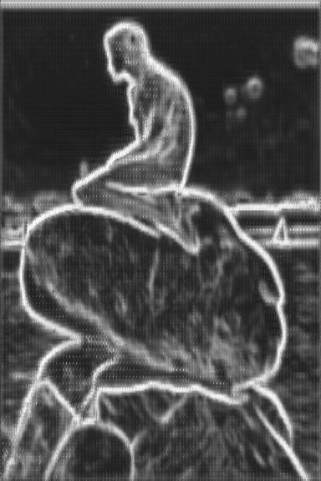
\includegraphics[width=0.24\textwidth]{../imagens/ilustracoes/cap6_bsds_372019_max_20200408.png}}
%   %\caption{Original image (a) and it borders detected by ALO-ADD (b), ALO-AVG (c) and ALO-MAX (d), using MORPH/UPPER ground truth methods.}
%   
%   \subfloat[Ground truth\label{fig:cap6_expr1_gt}]{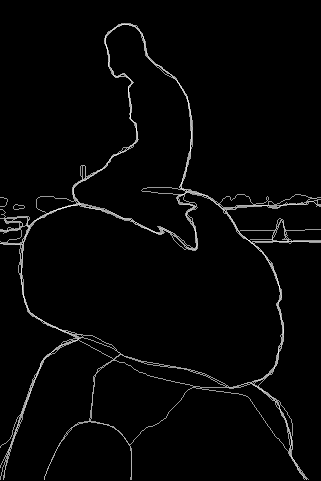
\includegraphics[width=0.24\textwidth]{../imagens/html/372019_upper.png}}
%   \hfill
%   \subfloat[ALO-ADD (0.47)\label{fig:cap6_expr1_add_th}]{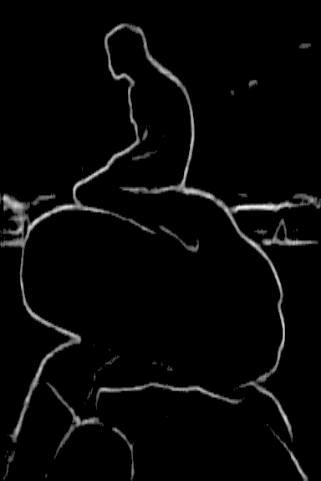
\includegraphics[width=0.24\textwidth]{../imagens/ilustracoes/cap6_bsds_372019_add_20200409_047.png}}
%   \hfill
%   \subfloat[ALO-AVG (0.46)\label{fig:cap6_expr1_avg_th}]{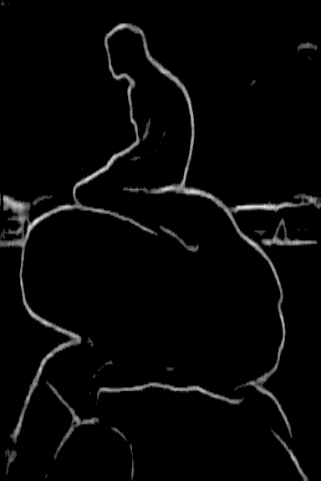
\includegraphics[width=0.24\textwidth]{../imagens/ilustracoes/cap6_bsds_372019_avg_20200407_046.png}}
%   \hfill
%   \subfloat[ALO-MAX (0.64)\label{fig:cap6_expr1_max_th}]{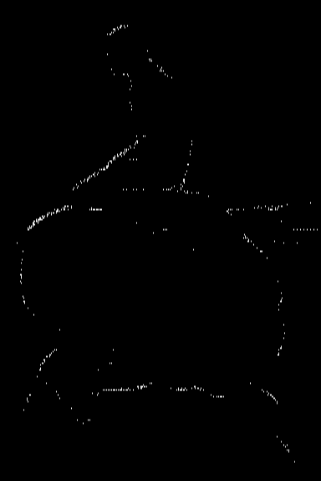
\includegraphics[width=0.24\textwidth]{../imagens/ilustracoes/cap6_bsds_372019_max_20200408_064.png}}
%   \caption{Predictions of the ALO-ADD, ALO-AVG and ALO-MAX networks, and its best thresholds.}
%   \label{fig:cap6_expr1_bsds_visual}
% \end{figure*}

%Figure \ref{fig:cap6_expr1_bsds_visual} shows that the predictions of ALO-ADD and ALO-AVG are quite similar, corroborating the results in Table \ref{tab:bsds_subexp1_results}.
%Also, the results shows that ALO-MAX didn't performed well, once it contains a lot of noise.
%Its best threshold removed many border details, resulting only in sparse pixels following the expected shape, but without producing a contour.

Due the weak convergence of ALO-MAX in all previous tests and preliminary experiments, it was decided that the ALO-MAX method will no longer be tested, due to its low performance.
The following sections will provide and discuss experiments using only the ALO-ADD and ALO-AVG methods.

%--------------------------------
\subsection{Experiment 2.2 - Improving Focal Loss and Hyperparameter Tuning}
\label{ssec:bsds_subexp2}

After training BSDS500 using Focal Loss, a new experiment was developed to try to increase the results achieved and decrease the number of training epochs.
To do it, a simple change in Focal Loss is proposed in this section.
The suggested change is to add the metric Pixel Error (PE), as a factor to improve Focal Loss (FL).

The purpose of the modification is to increase the separation between the edges and the background, making the network converge more quickly.
It is important to clarify that this change will mainly affect the ground truths MORPH and UPPER, that contains edge values far from background values.
This new metric, named PEFL, can be simple defined as Equation \ref{equ:pixel_error_focal_loss}:

\begin{equation}
  PEFL = FL \times (1 + PE)
  \label{equ:pixel_error_focal_loss}
\end{equation}

In conjunction with the new loss function, some hyper-parameter tuning were made\footnote{~The experiment described in Section \ref{ssec:bsds_subexp1} was performed again, changing only the loss function. It produced, using ALL and UPPER ground truths, 0.7502 and 0.7505 ODS values, with 429 (36\% less) and 460 (34\% less) epochs, respectively.}.
Some quick experiments were carried out and the one that showed the greatest evidence of improvement was the reduction in \textit{gamma} parameter.
Then, ALO-ADD and ALO-AVG networks were fully trained with the following changes in default parameterization, defined in Section \ref{ssec:framework_experiments}.

\begin{center}
Loss: PEFL ($\gamma$=1.0; $\alpha$=0.25)
\end{center}

% For the new experiment, the learning curves for MORPH phases are available in Figure \ref{fig:bsds_avg_fuse_1_morf}.
% It is noteworthy that ALO-AVG had, in all phases, a similar behavior to the network ALO-MAX in the experiment described in Section \ref{ssec:bsds_subexp1}.
% This unusual behavior, nonetheless, did not increase the number of training epochs nor decrease the performance.
% 
% \begin{figure}%[h!]
%   \centering
%   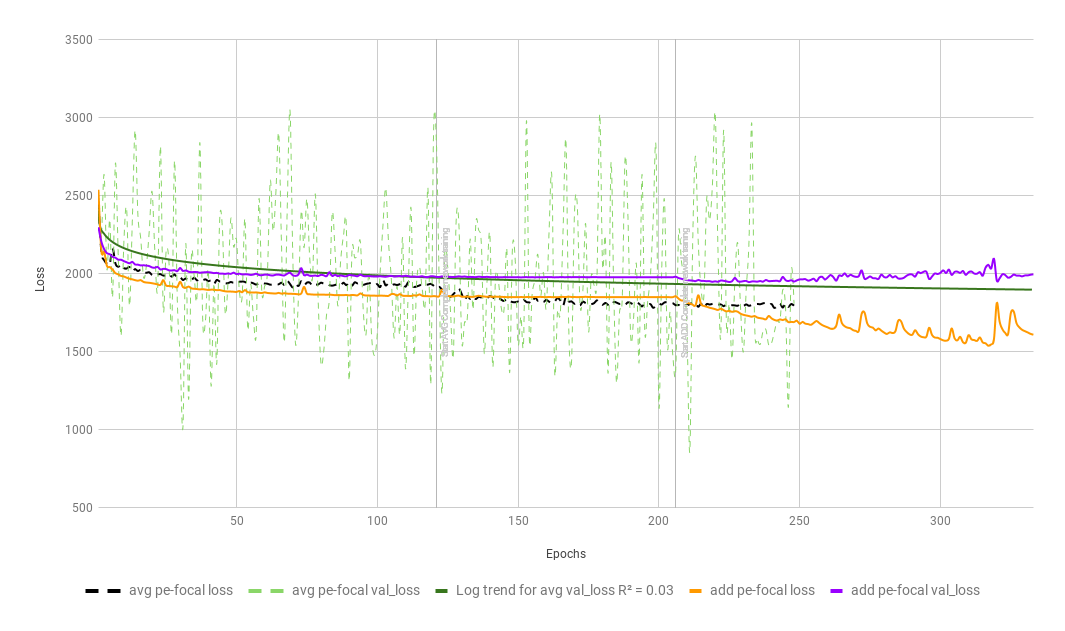
\includegraphics[width=1.\columnwidth]{../imagens/graficos/cap6_bsds_fuse_morf_v1v2_20200410-20.png}
%   \caption{Training and validation losses of ALO-ADD and ALO-AVG methods on BSDS500, using MORPH ground truth.}
%   \label{fig:bsds_avg_fuse_1_morf}
% \end{figure}

In the new experiment, ALO-AVG had, in all phases, a similar behavior to the network ALO-MAX in the experiment described in Section \ref{ssec:bsds_subexp1}.
This unusual behavior, nonetheless, did not increase the number of training epochs nor decrease the performance.
Instead, it performed better than that obtained in the experiment described in Section \ref{ssec:bsds_subexp1}, using the default parameterization, as can be seen in Table \ref{tab:bsds_subexp2_results}.

% The benchmark evaluation of ALO-AVG and ALO-ADD performances are available in Table \ref{tab:bsds_subexp2_results}.
% The number of training epochs are presented in Table \ref{tab:bsds_subexp2_epochs}.

\begin{table}%[h!]
  \centering
  \caption{Border detection performance on BSDS500 for ALO-ADD and ALO-AVG.}
  \scriptsize
  \setlength{\tabcolsep}{1em}
  \renewcommand{\arraystretch}{1.5}
  \begin{tabular}{{c}{c}{c}{c}{c}{c}{c}}
    \hline
    Network & Loss & Ground truth & TH & ODS & OIS %& Area PR
    \\
    \hline
    ALO-ADD & PEFL & ALL & 0.21 & 0.7558 & \textbf{0.7776} %& 0.6717
    \\
    ALO-ADD & PEFL & UPPER & 0.30 & 0.7559 & 0.7746 %& 0.6561
    \\
    \hline
    ALO-AVG & PEFL & ALL & 0.20 & 0.7546 & 0.7770 %& 0.6790
    \\
    ALO-AVG & PEFL & UPPER & 0.30 & \textbf{0.7563} & 0.7749 %& 0.673
    \\
    \hline
  \end{tabular}
  \label{tab:bsds_subexp2_results}
\end{table}

\begin{table}%[h!]
  \centering
  \caption{Number of training epochs of Pixel Error Focal Loss.}
  \scriptsize
  \setlength{\tabcolsep}{1em}
  \renewcommand{\arraystretch}{1.5}
  \begin{tabular}{{c}{c}{c}{c}{c}{c}{c}}
    \hline
    Ground truth & ALO-ADD & ALO-AVG 
    \\
    \hline
    MORPH / ALL & 553 & 409
    \\
    MORPH / UPPER & 620 & 473
    \\
    \hline
  \end{tabular}
  \label{tab:bsds_subexp2_epochs} 
\end{table}

Table \ref{tab:bsds_subexp2_epochs}  shows that the number of training epochs has decreased compared to the results of the previous training, available in Table \ref{tab:bsds_subexp1_epochs}.
Comparing the number of epochs of both experiments, it is possible to perceive that ALO-ADD reduced 16.97\% in MORPH/ALL method and 11.05\% in MORPH/UPPER method.
ALO-AVG performed even better, with reduction of training epochs for MORPH/ALL 36.19\% and 25.51\% for MORPH/UPPER ground truths.
It is important to remember that both networks have increased their performance when compared to previous experiments.

%--------------------------------
\subsection{Side-Outputs Contribution}
\label{ssec:bsds_sideout}

After training the network in previous experiments, it is important to evaluate the contributions of each layer.
Model interpretation can help decision making process to obtain knowledge to improve the model's performance \cite{Hohman:2019} and, also, improve results trustworthiness \cite{Chatzimparmpas:2020}.
%Contrary to what was done in Section \ref{cap6_contribuicoes_saidas_intermediarias}, where only the last layer of each stage was plotted, Figures \ref{fig:bsds_add_side_outputs} and \ref{fig:bsds_avg_side_outputs} displays information for all side-outputs of the networks.

Contrary to what was done in Section \ref{cap6_contribuicoes_saidas_intermediarias}, where only the last layer of each stage was plotted,
Figure \ref{fig:bsds_stage_outputs} combine results from side-outputs inside one distinct stage while Figure \ref{fig:bsds_stage_results} combine results of all previous stages, until the current one.
Figure \ref{fig:bsds_stage_outputs} helps to understand how each stage combine to the final output while \ref{fig:bsds_stage_results} helps to evaluate the gain when some stages are added to the final output.
Both images can contribute to the evaluation of a possible removal of stages in the network architecture.

% Then, Figure \ref{fig:bsds_stage_outputs} helps to understand how each stage combine to the final output while \ref{fig:bsds_stage_results} helps to evaluate the gain when some stages are added to the final output.
% Both images can contribute to the evaluation of a possible removal of stages in the network architecture.

% \begin{figure}%[h!]
%   \centering
%   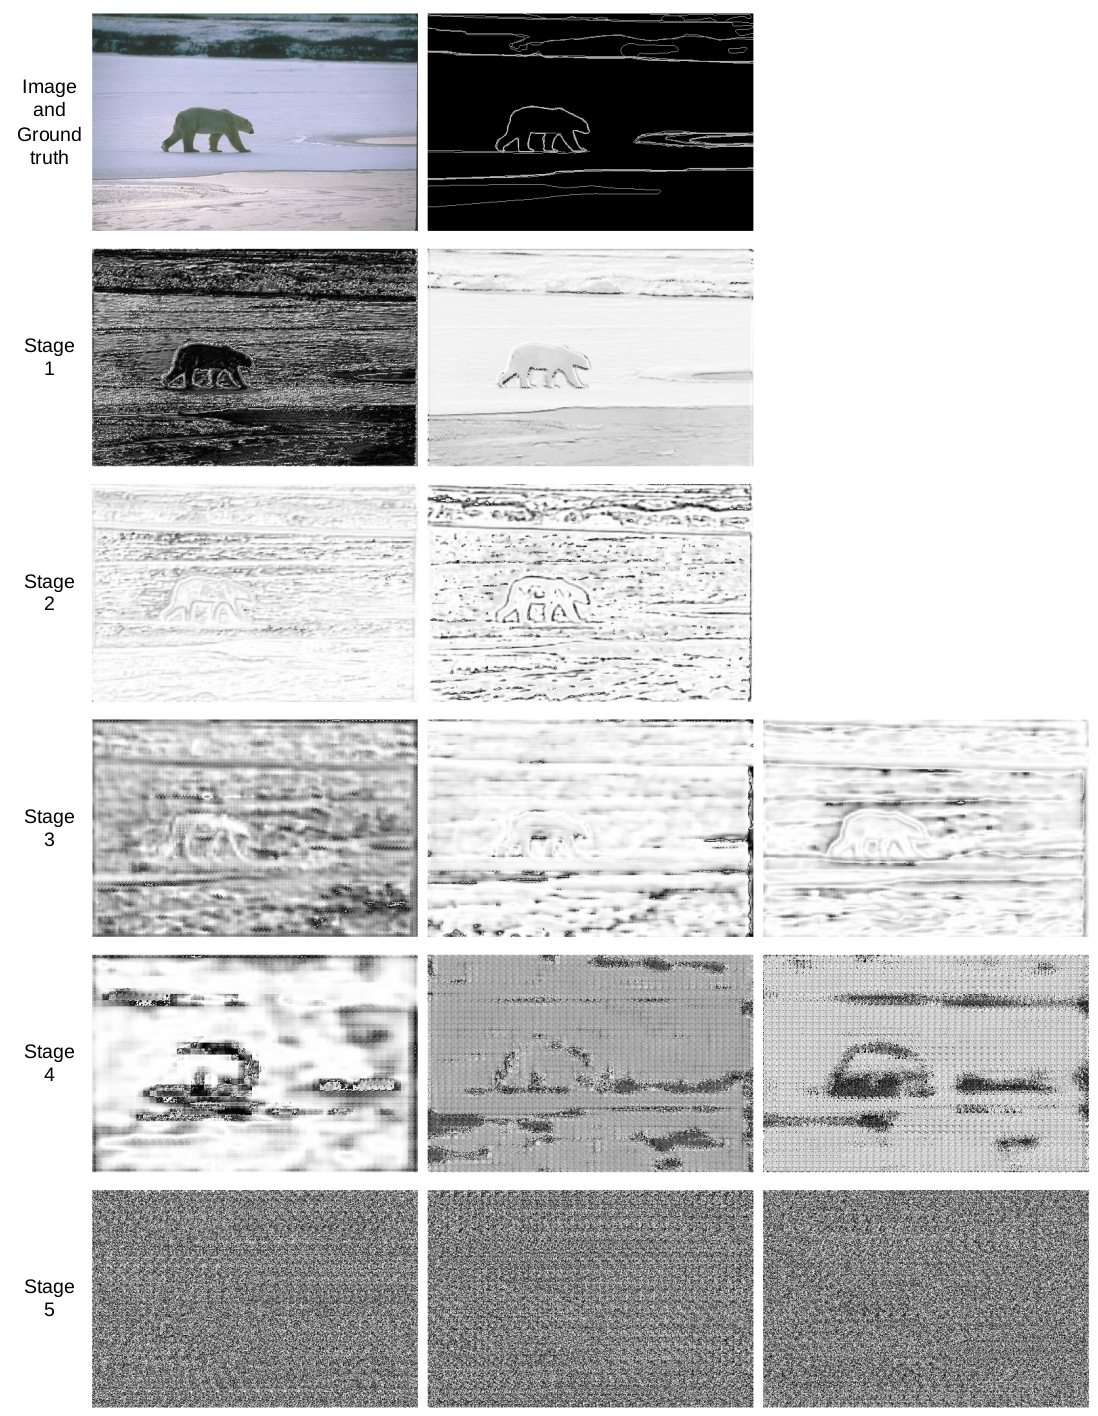
\includegraphics[width=1\columnwidth]{../imagens/ilustracoes/cap6_bsds_add_side_outputs.png}
%   \caption{Side-outputs of each convolution of ALO-ADD method, trained with BSDS 500 using MORPH/UPPER ground truth methods.}
%   \label{fig:bsds_add_side_outputs}
% \end{figure}
% 
% \begin{figure}%[h!]
%   \centering
%   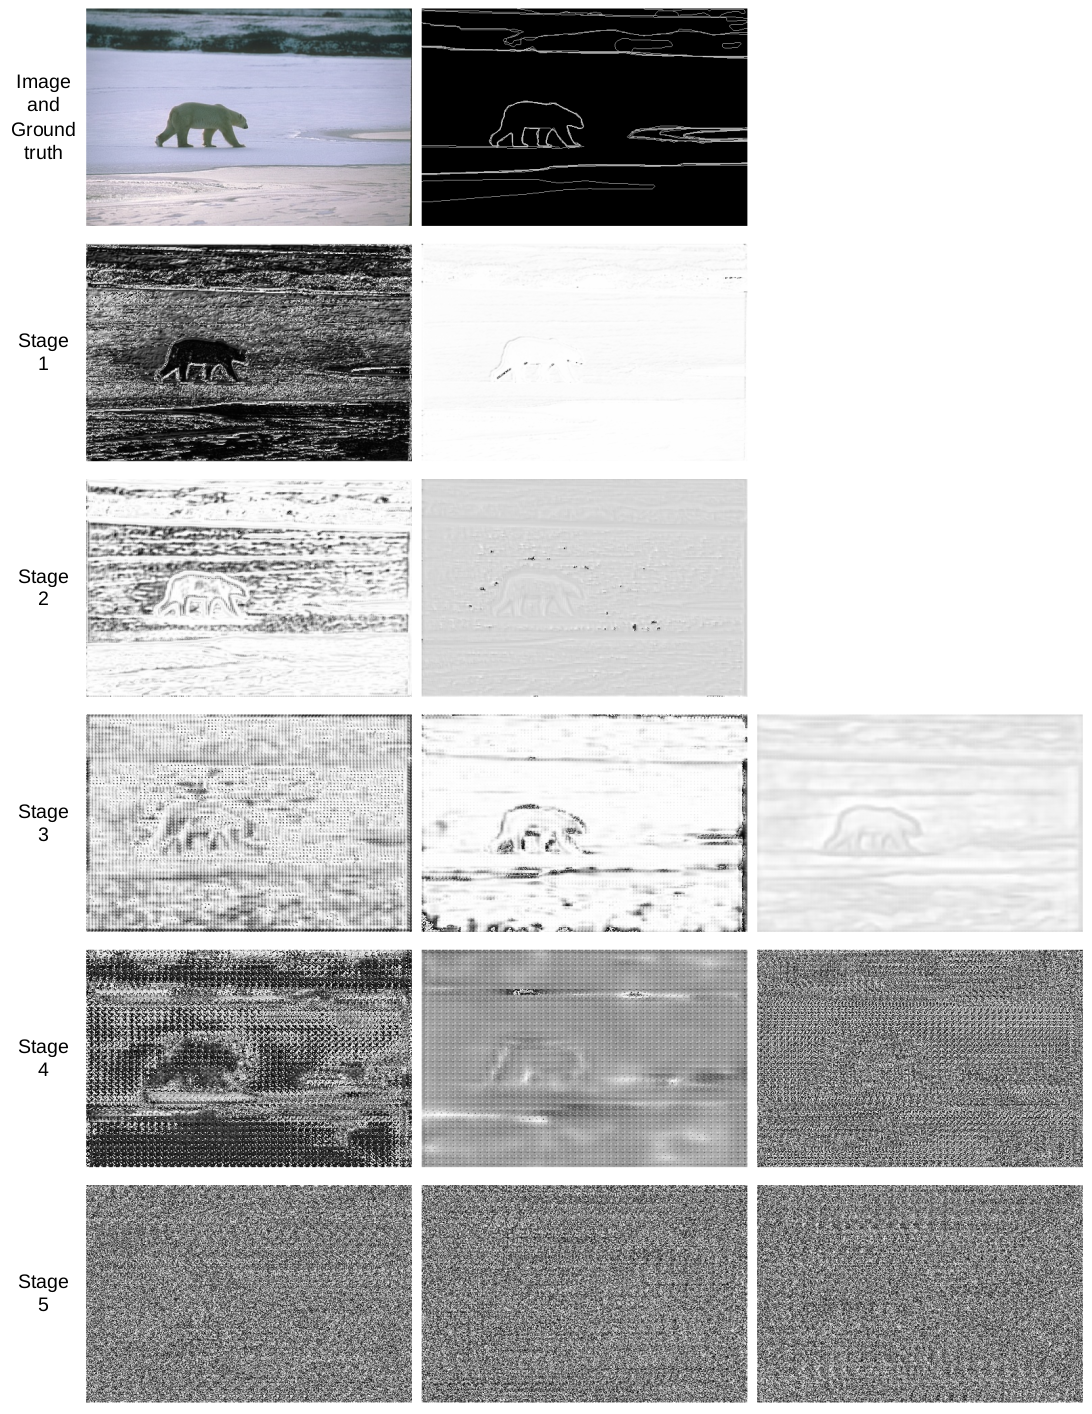
\includegraphics[width=1\columnwidth]{../imagens/ilustracoes/cap6_bsds_avg_side_outputs.png}
%   \caption{Side-outputs of each convolution of ALO-AVG method, trained with BSDS 500 using MORPH/UPPER ground truth methods.}
%   \label{fig:bsds_avg_side_outputs}
% \end{figure}

% It can be seen, in Figures \ref{fig:bsds_add_side_outputs} and \ref{fig:bsds_avg_side_outputs}, that the side-outputs of the first three stages are able to better identify the edges than the outputs of the final stages.

It can be seen, in Figures \ref{fig:bsds_stage_outputs} and \ref{fig:bsds_stage_results}, that the side-outputs of the first three stages are able to better identify the edges than the outputs of the final stages.
The last two stages only assist the results presented by the initial layers, and the latest one, in both networks, does not seen to have any important information for the network, only random noises.

It is also important to notice in Figure \ref{fig:bsds_stage_outputs} that most layers exhibit a large amount of light pixels (borders) compared to dark pixels (background).
This behavior can be considered unexpected, as the final result has borders and backgrounds in the correct colors and tones.
However, it is possible to see that the border, in most of them, is lighter than the surrounding colors, indicating an border.
Also, it was observed that the latest convolution, with operation of $1 \times 1$, described in Section \ref{cap5_saida_final_rede}, helps to separate these colors and tones, making the result close to the ground truth.

% Looking specifically at the first stage, with the assistance of Figures \ref{fig:bsds_add_side_outputs} and \ref{fig:bsds_avg_side_outputs}, it is noticed that both networks presents the same behavior.
% The first output present, in both networks, a dark image with general contours of the main object in the scene (a bear).
% Also, contains some noise, mainly in the background (ice/snow).
% The second outputs, contains the opposite characteristics, with an light image and some contours.
% ALO-ADD's second output shows better contours than those of the ALO-AVG, which presents low level of details.

% In the second stage, it is possible to see some differences to the first one.
% The image are clear, with more distinction of regions, due to color change.
% The images contains some noise, but in less quantity than observed in the first stage.
% ALO-AVG second output of this stage presents an image with few distinction between elements, in contrast to the other stage outputs in both networks.

% The third stage contains different results from ALO-ADD and ALO-AVG.
% ALO-ADD presents worse results than the first two stages, especially in the first and second side-output.
% The last output is the best of this stage, but it seems to be worse than the results of the previous stages, in terms of details.
% The first two outputs of ALO-AVG can be compared to those of ALO-ADD, with low performance .
% However, the last output has possibly the best result of all analyzed ALO-AVG side-outputs.

% It is possible to see in Figures \ref{fig:bsds_add_side_outputs} and \ref{fig:bsds_avg_side_outputs} that the last two stages has small contribution to the final output, when compared to the previous ones.
% The fourth stage contains results with little precision, showing only blots in some regions of interest.
% The fifth stage shows only random noises, which probably have little help in improving the results.

% Help to evaluate the results produced by the side-outputs when combined, are presented Figures \ref{fig:bsds_stage_outputs} and \ref{fig:bsds_stage_results}.
% Figure \ref{fig:bsds_stage_outputs} combine results from side-outputs inside one distinct stage while Figure \ref{fig:bsds_stage_results} combine results of all previous stages, until the current one.
% Then, Figure \ref{fig:bsds_stage_outputs} helps to understand how each stage combine to the final output while \ref{fig:bsds_stage_results} helps to evaluate the gain when some stages are added to the final output.
% Both images can contribute to the evaluation of a possible removal of stages in the network architecture.

\begin{figure}%[h!]
  \centering
  %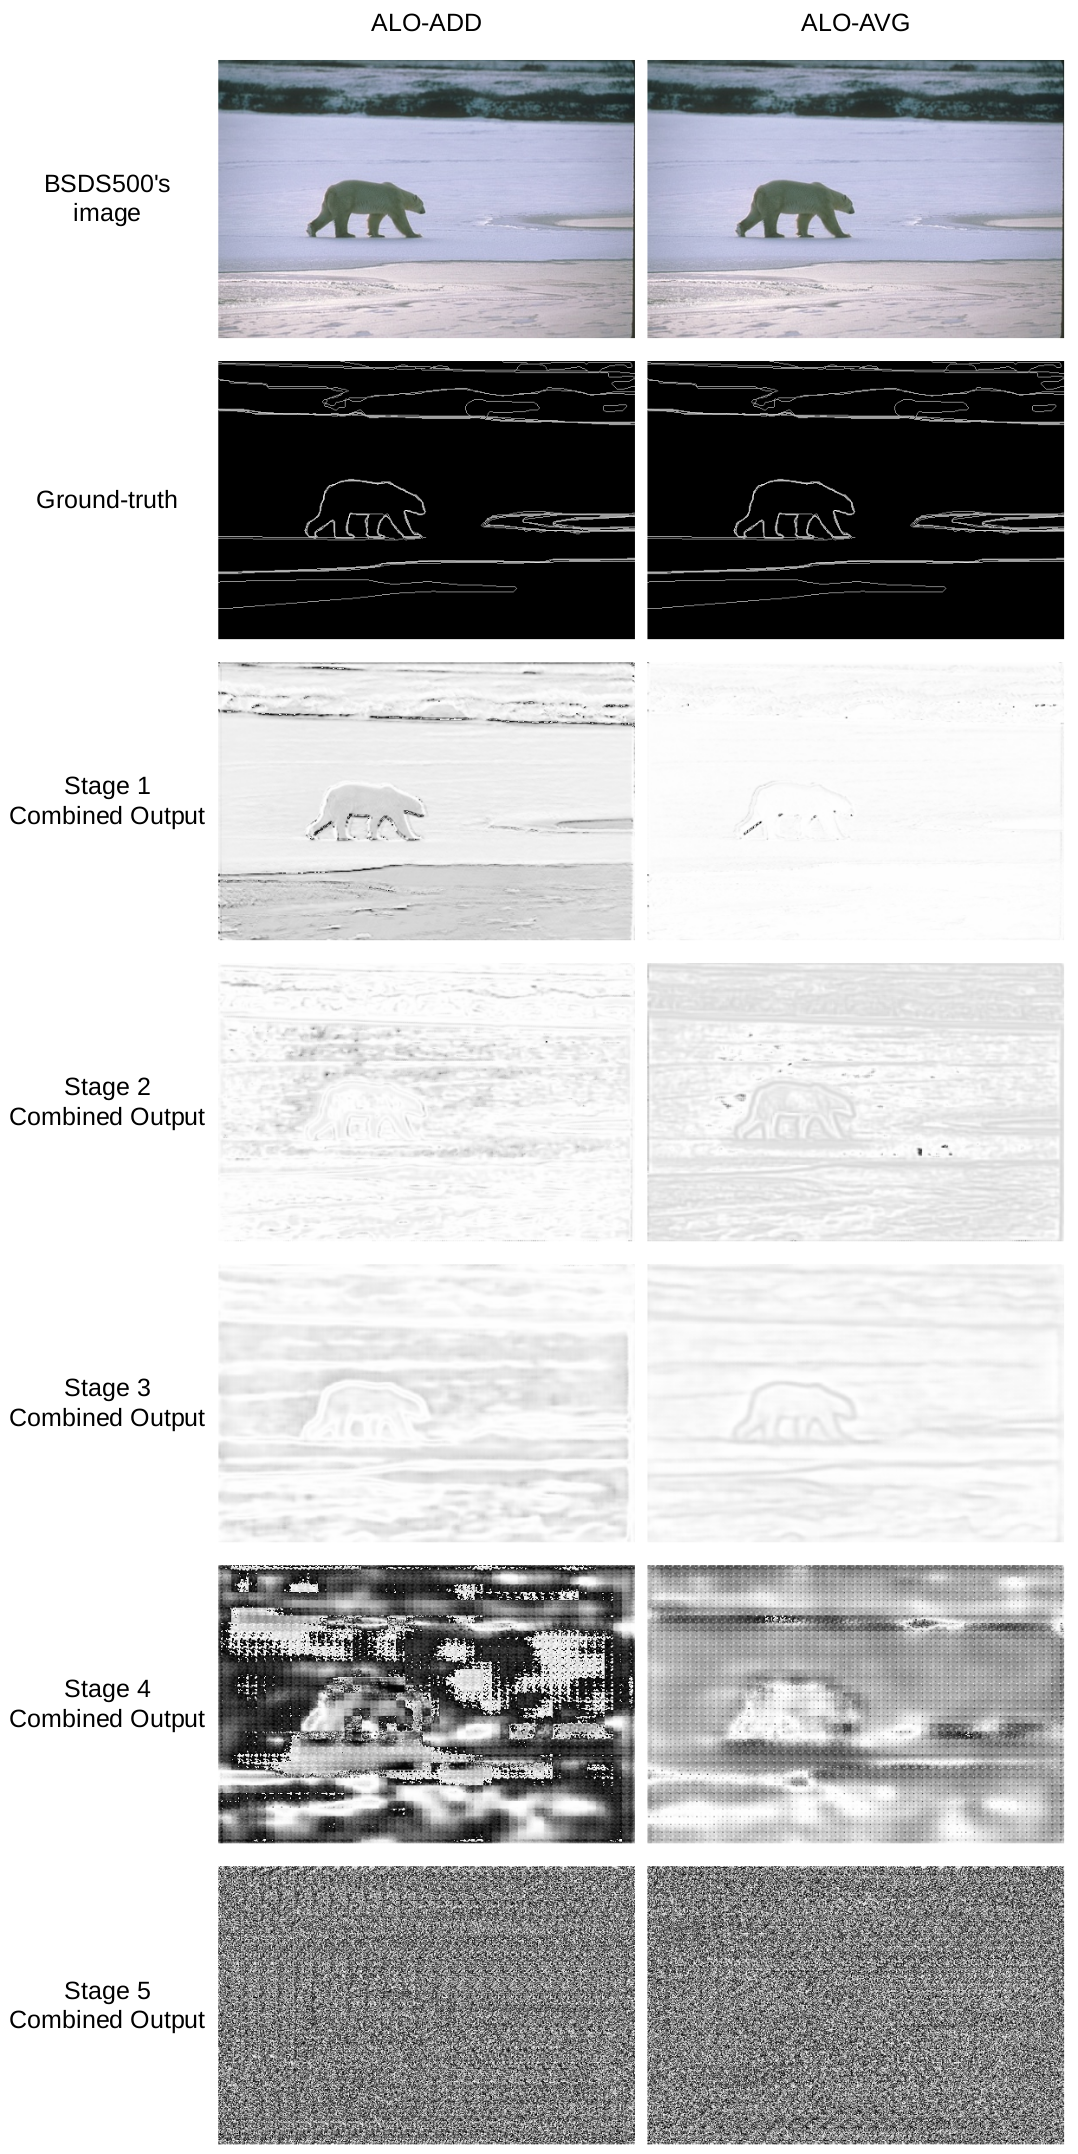
\includegraphics[width=0.9\columnwidth]{../imagens/ilustracoes/cap6_bsds_stage_outputs.png}
  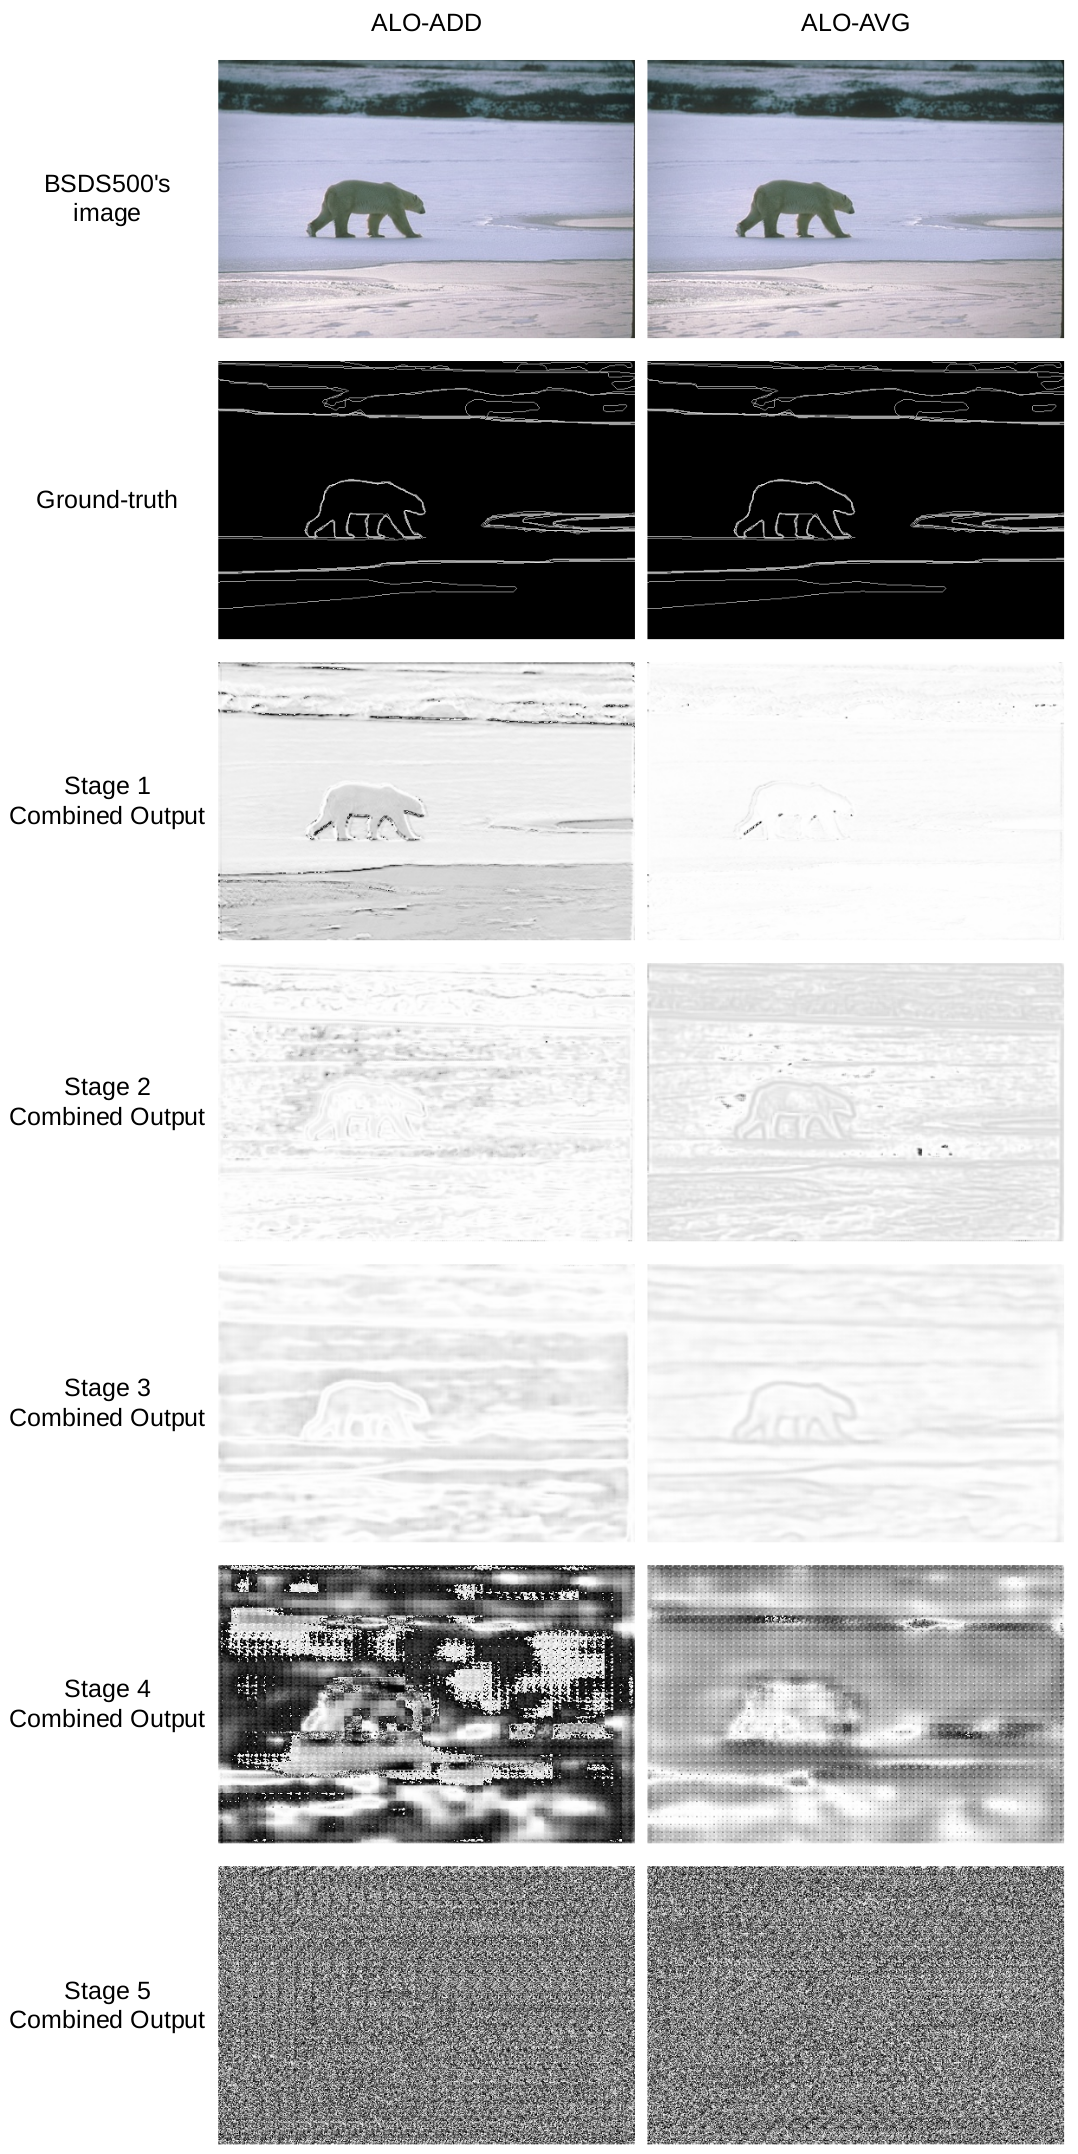
\includegraphics[width=1\columnwidth]{../imagens/ilustracoes/cap6_bsds_stage_outputs.png} %VISUALIZ
  \caption{Side-outputs of each stage of ALO-ADD and ALO-AVG methods, trained with BSDS 500 using MORPH/UPPER ground truth methods.}
  \label{fig:bsds_stage_outputs}
\end{figure}

\begin{figure}%[h!]
  \centering
  %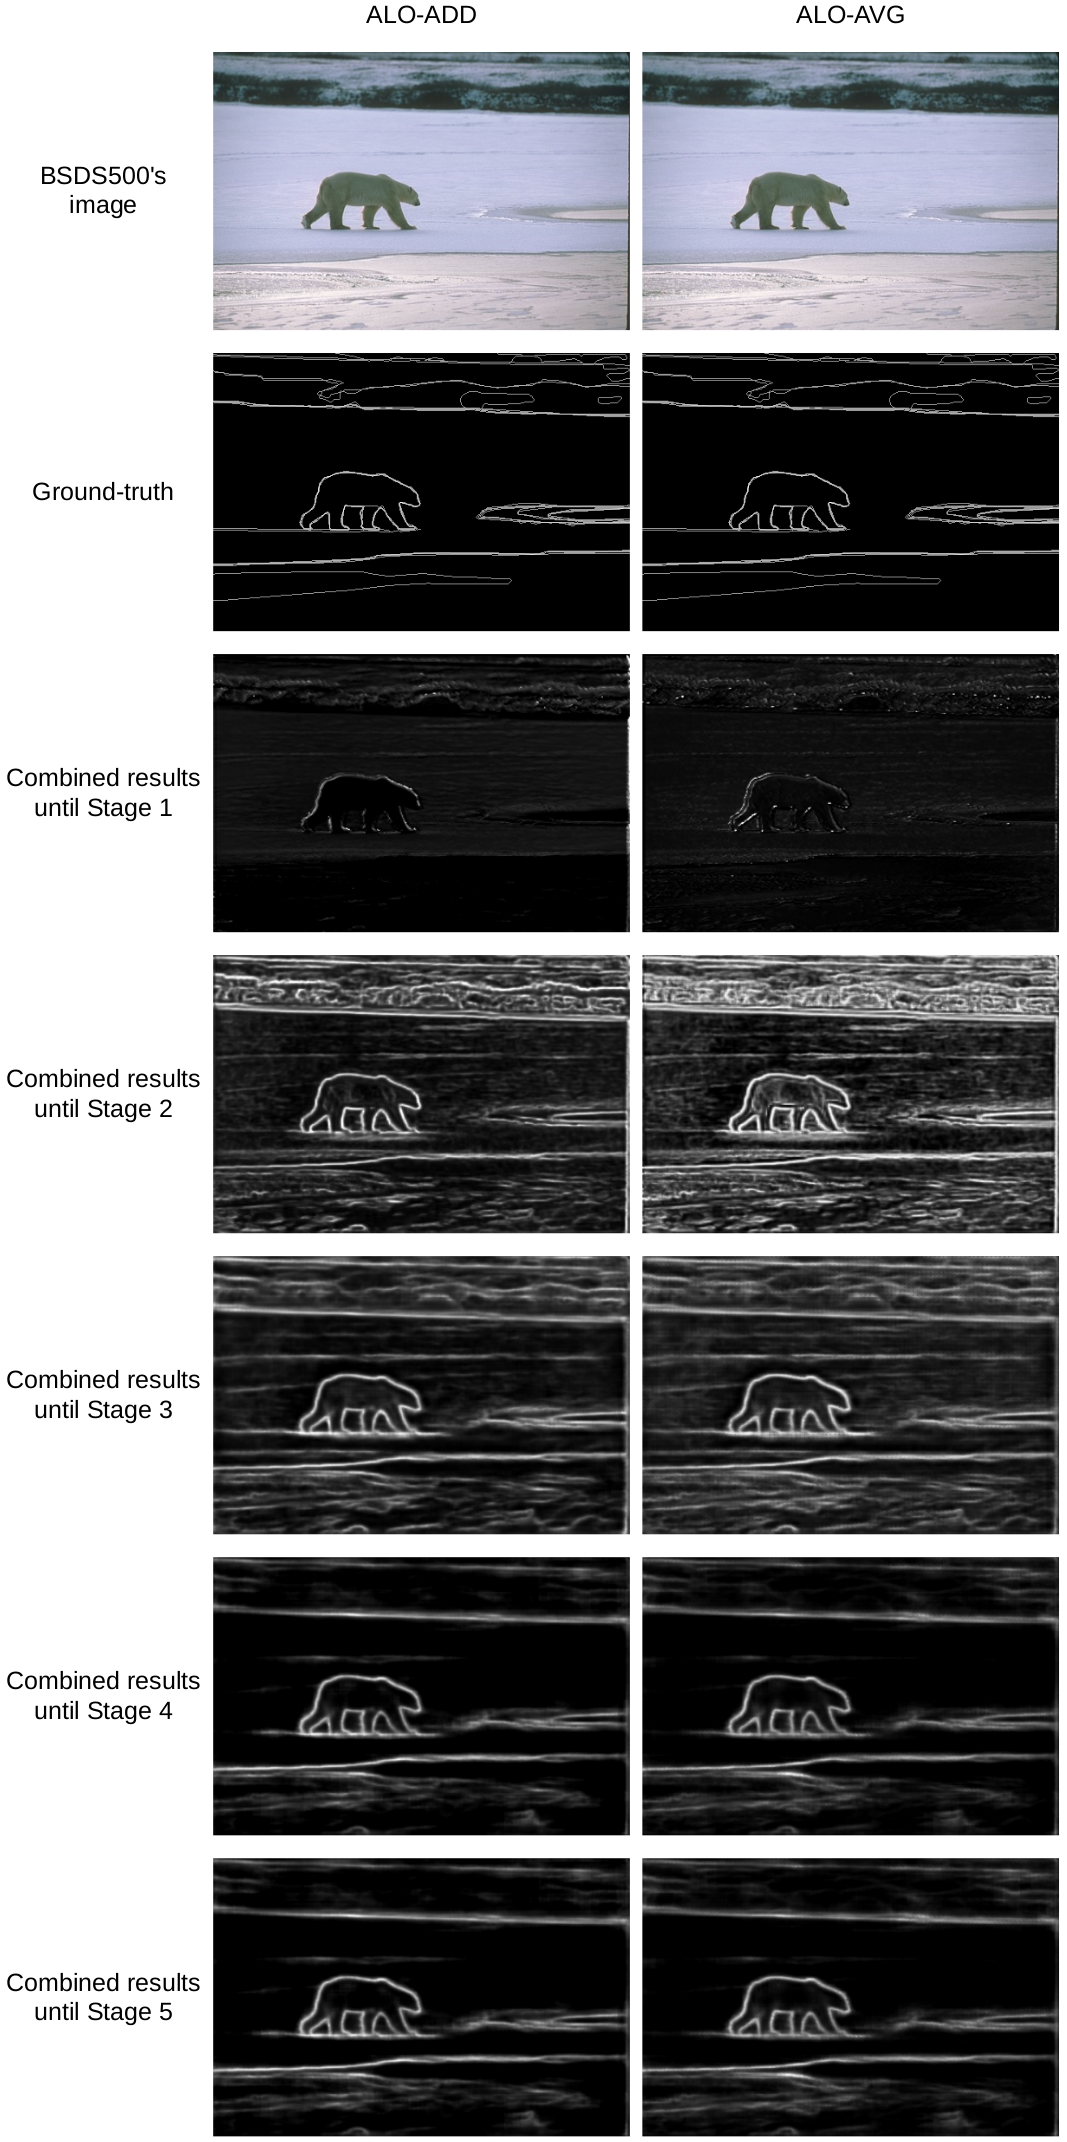
\includegraphics[width=0.9\columnwidth]{../imagens/ilustracoes/cap6_bsds_stage_results.png}
  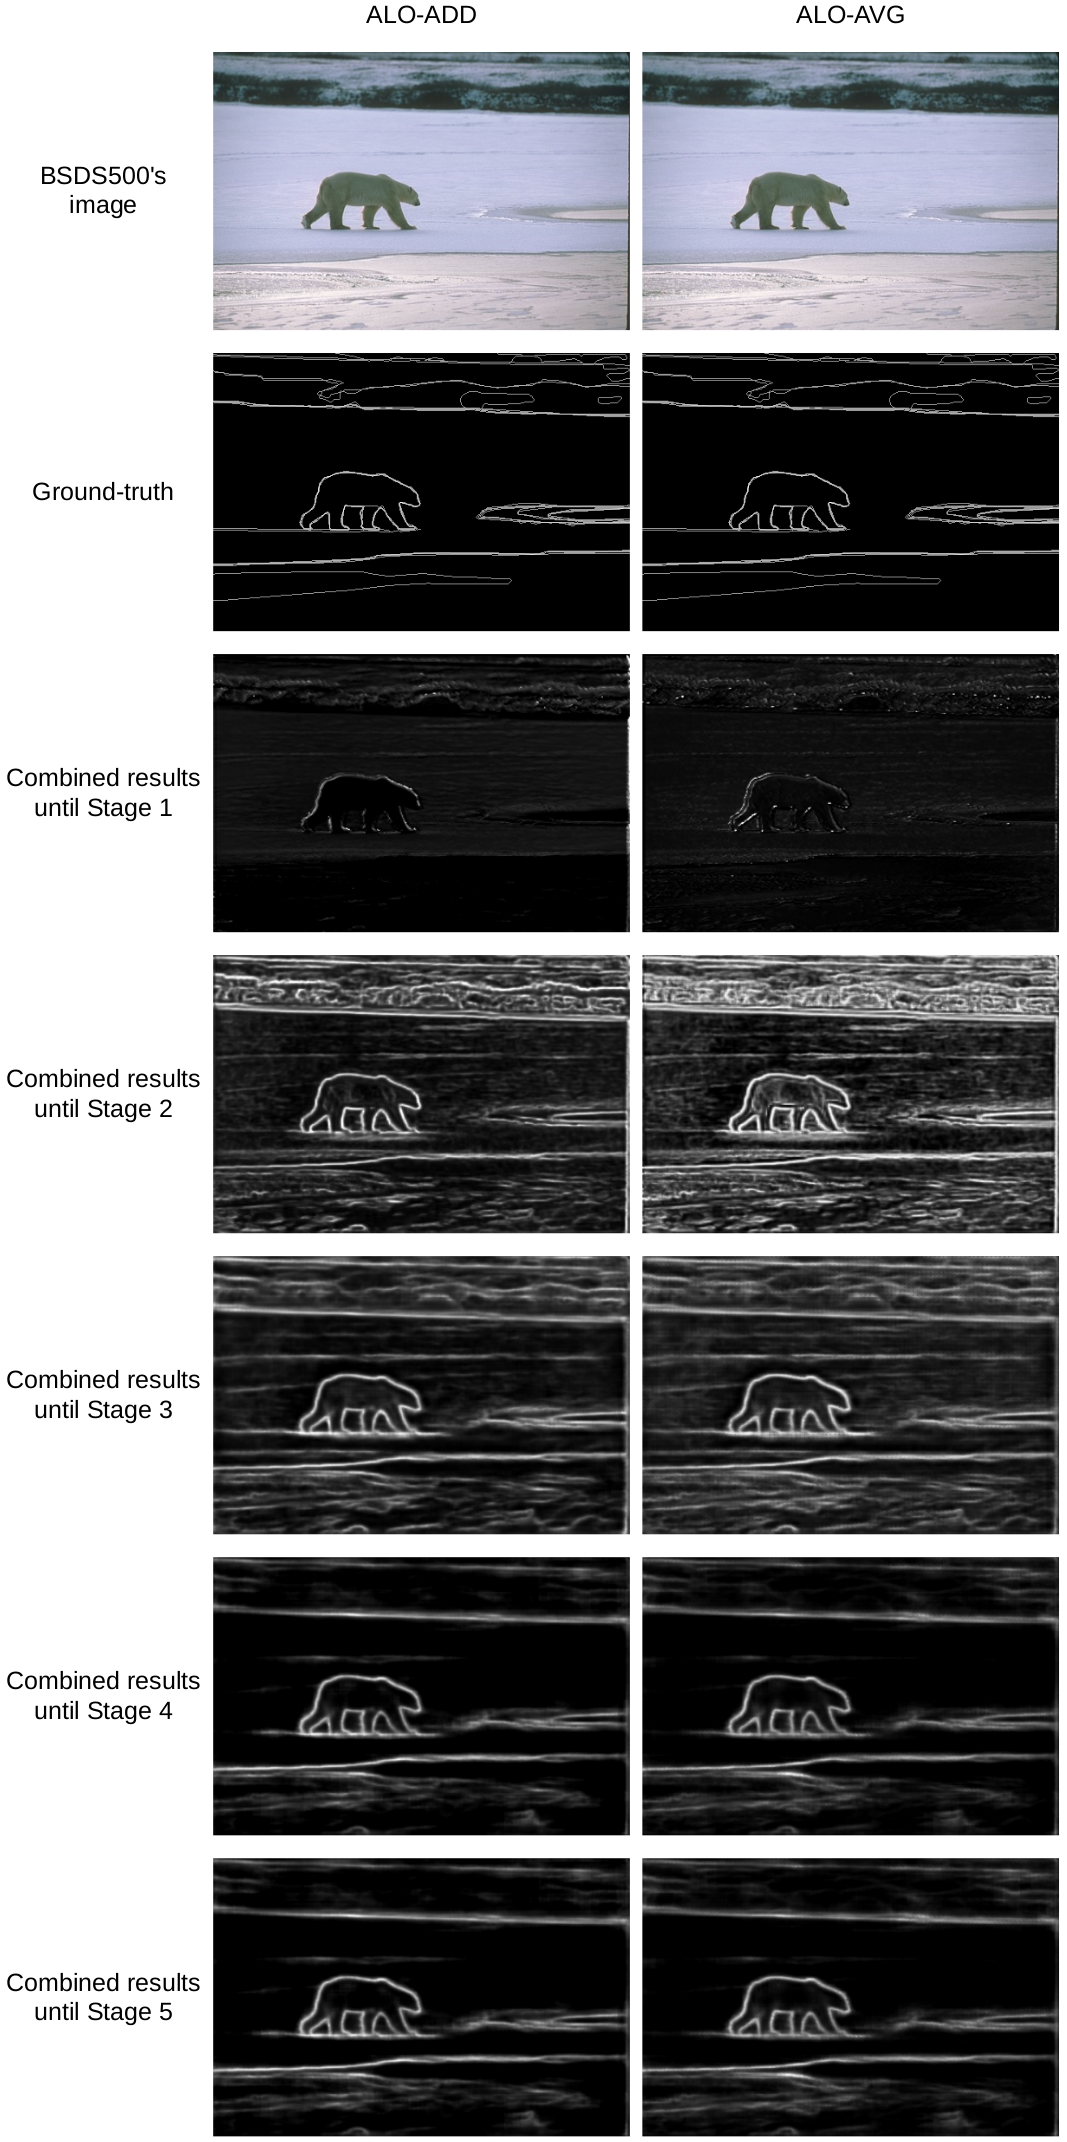
\includegraphics[width=1\columnwidth]{../imagens/ilustracoes/cap6_bsds_stage_results.png} %VISUALIZ
  \caption{Results of ALO-ADD and ALO-AVG methods with side-outputs until each stage, trained with BSDS 500 using MORPH/UPPER ground truth methods.}
  \label{fig:bsds_stage_results}
\end{figure}

% It can be seen in Figure \ref{fig:bsds_stage_outputs} that ALO-ADD and ALO-AVG have different stage output contributions.
% ALO-ADD appears to perform better in stages 1 and 3, while ALO-AVG appears to perform better in stages 2 and 3.
% In the fourth stage, the results shows only blurs, but it is possible to identify some parts only in ALO-AVG, with appears to contribute more with the final output.
% The last stage, as already observed in Figures \ref{fig:bsds_add_side_outputs} and \ref{fig:bsds_avg_side_outputs}, presents only random noises.

Figure \ref{fig:bsds_stage_results} shows a different perspective of stage outputs contribution.
It can be seen that the results become more accurate as more stages are added, except for the last stage, which apparently does not improve the overall performance of the model.

%--------------------------------
\subsection{Experiment 2.3 - Removing last stage layers}
\label{ssec:bsds_subexp3}

After analyzing the intermediate results, as indicated in Section \ref{ssec:bsds_sideout}, a new experiment was developed with the purpose of evaluating the impact of removing layers from the last stage.
As observed in Figures \ref{fig:bsds_stage_outputs} and \ref{fig:bsds_stage_results}, the layers of the fifth stage apparently does not contribute effectively to the final result.

In this experiment, the same parameterization described in Section \ref{ssec:bsds_subexp2} was used, except for the loss decreasing and the minimum learning rate (MinLR).
The value, once fixed into $1 \times 10^{-9}$, was replaced by Equation \ref{eq:min_lr}, where the value depends of the original Learning Rate.
This procedure reduced it to $1 \times 10^{-10}$ in the first phase and $1 \times 10^{-11}$ in last two phases of the protocol.

\begin{equation}
  MinLR = LR \times 10^{-4}
  \label{eq:min_lr}
\end{equation}

Once ALO-AVG and ALO-ADD had similar performance in the previous tests, it was decided to evaluate only one of the methods.
Due to the better performance in the ODS metric, with fewer training epochs, according to Section \ref{ssec:bsds_subexp2}, ALO-AVG was chosen to be used in the following experiments.
Then, ALO-AVG network was completely trained using the protocol defined in Section \ref{ssec:framework_experiments} and the parameterization recently defined.

The 4 and 5-stages ALO-AVG networks had similar values in the first phase of the protocol.
In the second phase, the 4-stage network contains considerably lower losses.
This pattern is also manifest in the last phase, using ALL ground truth.
As results of the lower loss, the 4-stage network produced better results, as described in Table \ref{tab:bsds_subexp3_results}, despite of the bigger number of epochs to reach the best value.

The network training process of the 4-stage ALO-AVG method was carried out in 556 epochs, instead of 409 from regular 5-stages ALO-AVG.
As the network with 4 layers is smaller than the traditional network, each epoch runs faster.
However, even with this advantage, the total training time was about 21.80\% longer than conventional 5-stage ALO-AVG.

% The network training and its comparison with 5-stage ALO-AVG are available in Figures \ref{fig:bsds_4stage_morph} and \ref{fig:bsds_4stage_all}.
% Figure \ref{fig:bsds_4stage_morph} shows similar values for both networks in the first phase of the protocol.
% In the second phase, the 4-stage network contains considerably lower losses.
% This pattern is also manifest in the last phase, using ALL ground truth, as presented in Figure \ref{fig:bsds_4stage_all}.

%Tempo: s4 = 43084+123229+99740=266053 | s5 = 37266+80641+100524=218431

% \begin{figure}%[h!]
%   \centering
%   \includegraphics[width=1.\columnwidth]{../imagens/graficos/cap6_bsds_avg_4stage_morph_20200410-0529.png}
%   \caption{Training losses of 4 and 5 stages ALO-AVG versions using MORPH ground truth on BSDS500.}
%   \label{fig:bsds_4stage_morph}
% \end{figure}
% 
% \begin{figure}%[h!]
%   \centering
%   \includegraphics[width=1.\columnwidth]{../imagens/graficos/cap6_bsds_avg_4stage_all_20200410-0529.png}
%   \caption{Training losses of 4 and 5 stages ALO-AVG versions using ALL ground truth on BSDS500.}
%   \label{fig:bsds_4stage_all}
% \end{figure}

% As results of the lower loss, the 4-stage network produced better results, as described in Table \ref{tab:bsds_subexp3_results}, despite of the bigger number of epochs to reach the best value.

\begin{table}%[h!]
  \centering
  \caption{Border detection performance on BSDS500 for ALO-AVG with 4 stages.}
  \scriptsize
  \setlength{\tabcolsep}{1em}
  \renewcommand{\arraystretch}{1.5}
  \begin{tabular}{{c}{c}{c}{c}{c}{c}}
    \hline
    Network & Loss & Ground truth & TH & ODS & OIS
    \\
    \hline
    ALO-AVG & PEFL & ALL & 0.17 & 0.7625 & 0.7791
    \\
    \hline
  \end{tabular}
  \label{tab:bsds_subexp3_results}
\end{table}

\subsubsection{Changing data pre processing}
\label{sssec:bsds_pre_process_data}

All previous experiments, including those with the KITTI data set, were done using histogram equalization for each image channel as a pre-processing step.
The technique was chosen due to its possible adaptation to different databases.
However, after all the experiments previously carried out, it was decided to evaluate the subtraction of the means of each channel, using the same parameters described in \cite{VGGNET:2014} paper.

Using VGGNet pre-processing weights, an increase in performance was expected, since the method would equalize the entire database evenly, unlike the previous technique, which adjusted each image separately.
Such a procedure would enable faster and more effective learning.

To assess the change, a naive test was performed using the final weights from the previous experiment.
The network was trained again, only in the last phase of the protocol, using images with the new pre-processing method.
Surprisingly, only this step was able to raise previous results by more than 1\%, to 0.7769 ODS and 0.7913 OIS values.

In order to provide a fair comparison, the network was fully trained using the same parameters described in experiment of Section \ref{ssec:bsds_subexp3}.
The training procedure left 490 epochs and produced the results in Table \ref{tab:bsds_subexp3_results_pre_vgg}.
The results are slightly inferior to training described in the last paragraph, but once it followed the fully protocol, it better represent the behavior of the network.

\begin{table}%[h!]
  \centering
  \caption{Border detection performance on BSDS500 for ALO-AVG with 4 stages, using VGG16 pre-processing.}
  \scriptsize
  \setlength{\tabcolsep}{1em}
  \renewcommand{\arraystretch}{1.5}
  \begin{tabular}{{c}{c}{c}{c}{c}{c}}
    \hline
    Network & Loss & Ground truth & TH & ODS & OIS
    \\
    \hline
    ALO-AVG & PEFL & ALL & 0.18 & 0.7735 & 0.7876
    \\
    \hline
  \end{tabular}
  \label{tab:bsds_subexp3_results_pre_vgg}
\end{table}

The results provided in this section indicates that the change in the pre-processing method increased the results and reduced the number of training epochs, as expected.
%These results indicates the influence of the data set equalization.
The following experiments, in next sections, will use the same pre-processing method.
  
%--------------------------------
% \subsection{Experiment 2.4 - Training Side-Outputs}
% \label{ssec:bsds_subexp4}
% 
% In order to answer Research Question Q2, described in Section \ref{cap1_objetivos}, and Hypothesis H3, detailed in Section \ref{cap1_hipoteses}, a new experiment was developed.
% The experiment aims to evaluate the contribution of the technique of forcing side-outputs to produce similar predictions, in order to take advantage of multi-scale architecture.
% 
% To evaluate this technique, a new experiment was developed, with different ways of forcing the neural networks to produce the same result at the side-outputs, to try take advantage of multi-scale inside the network.
% All networks used in this experiment were versions of VGG16 with 4 stages and parameterization similar to that described in Section \ref{ssec:bsds_subexp3} (including  pre-processing described in Section \ref{sssec:bsds_pre_process_data}).
% 
% \subsubsection{Training each convolution of ALO-AVG with 4 stages}
% \label{sssec:train_conv_alo_avg}
% 
% The first experiment aimed to evaluate the possible improvement in the results of the ALO-AVG network by training it with loss functions after each convolutional layer.
% The network was then trained with 11 loss functions, one for each convolution and one for the final output, with the average result of the entire network.
% 
% This training variation sought to evaluate the gains in the production of multi-scale outputs with the network that obtained the best results in the previous experiments.
% However, despite the good results in the previous experiments, the network had difficulties to learn, possibly due to the excess of outputs and loss functions.
% 
% Excessive side-outputs may have caused difficulties in the transmission of knowledge between layers of the network.
% The color and border adjustments, as shown in Figure \ref{fig:bsds_avg_side_outputs}, were compromised, since the layer alone sought to generate an output close to the border map.
% 
% It was observed, in the individual evaluation of the outputs, that some intermediate results, mainly in the first stages, did not present useful information (map without any border) and that several others, mainly at the end of the network, presented many noises, generating many false positives and inaccurate edges.
% 
% As result, the network produced, in a only 271 epochs training, an ODS value of 0.7259 and an OIS value of 0.7418, considerably lower than the results obtained in Section \ref{sssec:bsds_pre_process_data}.
% The low number of training epochs, added to the low results obtained, indicates that the network was unable to learn properly and that the high number of side-outputs hindered learning.
% 
% \subsubsection{Training each stage of SLO-AVG with 4 stages}
% \label{sssec:train_stage_slo_avg}
% 
% Due to the poor results of the ALO-AVG network in the last experiment, it was proposed to reduce the number of side-outputs that should be trained.
% Following the context of this work and the previously used networks, it was decided to use the SLO-AVG net.
% The network was trained with 5 loss functions, one for each stage and one for the final average output.
% 
% Since early epochs, this version of the network produced smaller training and validation loss values than the previous ALO-AVG experiment.
% After 476 training epochs, the network produced 0.7640 ODS and 0.7795 OIS values, which is almost 6\% better than the last experiment with ALO-AVG.
% Nonetheless, these results are smaller than the results of ALO-AVG without multiple loss functions, as described in Section \ref{sssec:bsds_pre_process_data}.
% 
% \subsubsection{Training a fine and a coarse output}
% \label{sssec:train_alo_plus}
% 
% Inspired in Convolutional Oriented Boundaries network \cite{COB:2016}, this new experiment aimed to evaluate the creation of a fine and a coarse output.
% To produce it, a new version of ALO-AVG network was created and named ALO-PLUS.
% 
% The network contained two side-outputs, a fine one, containing the average of the initial intermediate outputs (convolutions in stages 1 to 3) and a coarse one, containing the average of the outputs of the fourth stage.
% The outputs were trained independently.
% To produce a single result, a late merging method was created, with the average of both results.
% 
% The BSDS500 evaluation of the results produced by this ALO-PLUS network resulted in 0.7573 ODS and 0.7729 OIS values (the training procedure left 534 epochs).
% The results can be considered intermediate when compared to values of other experiments carried out in this work.
% 
% It is also important to indicate that this experiment, with a delayed fusion method, allows the choice of a more appropriate technique to combine the network outputs after training.
% Despite this, only a visual assessment of the use of weights in each output was made, but no improvement was noticed. 
% Then, it was not evaluated using the BSDS500 benchmark.
% 
% \subsubsection{Training each stage of SLO-ADD  with 4 stages}
% \label{sssec:train_stage_slo_add}
% 
% Due to the good results of the SLO-AVG network in the experiment described in Section \ref{sssec:train_stage_slo_avg} and the equivalence of ADD and AVG methods in some experiments described in Sections \ref{ssec:bsds_subexp2} and \ref{ssec:bsds_subexp2}, a new experiment was carried out using SLO-ADD network.
% The network was trained with 5 loss functions, one for each stage and one for the final output.
% 
% The training of SLO-ADD was slower to other networks, with exactly 700 epochs.
% Despite the longer training time, SLO-ADD produced poorly 0.7117 ODS and 0.7231 OIS values, what is considerably worse than SLO-AVG and other networks.
% 
% The results visually indicated the edges, however, presented numerous noises, which could be considered as soft edges.
% However, it was noticed that the hue of the soft edges was very similar to the hard edges, which probably caused the results to be very low.
% This small difference could lead to multiple false positives, even with different thresholds.
% 
% \subsubsection{Side-outputs training summary}
% \label{sssec:sideout_train_summary}
% 
% The summary of the experiments performed in this section are presented in Table \ref{tab:bsds_subexp4_results}.
% Analyzing the results, it is possible to see that SLO-AVG network had the best ODS and OIS values.
% However, the results are smaller than those achieved by ALO-AVG net in Section \ref{sssec:bsds_pre_process_data}.
% 
% \begin{table}%[h!]
%   \centering
%   \caption{Border detection performance on BSDS500 for SLO and ALO networks with side-output training.}
%   \scriptsize
%   \setlength{\tabcolsep}{1em}
%   \renewcommand{\arraystretch}{1.5}
%   \begin{tabular}{{c}{c}{c}{c}{c}{c}{c}}
%     \hline
%     Network & Loss & Trained side-outputs & Ground truth & TH & ODS & OIS
%     \\
%     \hline
%     ALO-AVG & PEFL & 11 & ALL & 0.18 & 0.7259 & 0.7418
%     \\
%     SLO-AVG & PEFL & 5 & ALL & 0.18 & 0.7640 & 0.7795
%     \\
%     ALO-PLUS & PEFL & 2 (fine and coarse) & ALL & 0.18 & 0.7573 & 0.7729
%     \\
%     SLO-ADD & PEFL & 5 & ALL & 0.18 & 0.7117 & 0.7231
%     \\
%     \hline
%   \end{tabular}
%   \vspace{0.2cm}
%   \label{tab:bsds_subexp4_results}
% \end{table}

%--------------------------------
\subsection{Experiment 2.5 - Improving ALO network}
\label{ssec:bsds_subexp5}

% After analyse the experiments in Section \ref{ssec:bsds_subexp3}, and inspired in some recent papers that create auxiliary branches in their network, as \cite{Cumulative:Song20181847}, \cite{LearningHybrid:Hu2018377} and \cite{He:2019}, a new experiment was proposed.
% To create an auxiliary branch, the first step was adding some new convolutional layers in each side-output of the 4-stage ALO network.
% 
% The network was trained with this new architecture for a few epochs and, before evaluate the results, it was observed that the loss increased and the network also left more training epochs to converge properly.
% After review the side-output block, it was decided to counter the recent trend of auxiliary branches and remove each possible extra layer of that block.

As described in Section \ref{cap5_saidas_laterais}, ALO's side-output blocks are composed by an $1 \times 1$ convolution, followed by a transposed convolution.
It was observed that the $1 \times 1$ convolution could be removed without great impact in the network, except for the possibility of making it a little less stable.

Due to the architectural change made and in order to differentiate it from the ALO network, the new neural network was named \textit{eXtreme All-layers Outputs}  (XLO).
% The network was created only with AVG and ADD operations, due the poor performance of MAX in previous tests, as described in Sections \ref{ssec:bsds_subexp1} and \ref{ssec:basic_pred_eval}.
% The XLO network was trained using the default protocol with AVG and ADD merging methods, ALL and UPPER ground truths and the following parameterization, similar to that described in Section \ref{sssec:bsds_pre_process_data}, and summarized below.
The XLO network was trained using the default protocol with AVG and ADD merging methods, ALL and UPPER ground truths and the following parameterization different from the default one, described in Section \ref{ssec:framework_experiments}.

\begin{itemize}
  \item Learning rate: $1 \times 10^{-6}$ (first step) and $1 \times 10^{-7}$ (others)
  \item Learn. decay: $1 \times 10^{-10}$ (first step) and $1 \times 10^{-11}$ (others)
  \item Loss: PEFL ($\gamma$=1.0; $\alpha$=0.25)
  \item Pre-processing: VGG-16
\end{itemize}

% \begin{itemize}
%   \item Learning method: SGD
%   \item Activation: ReLU
%   \item Learning rate: $1 \times 10^{-6}$ (first step) and $1 \times 10^{-7}$ (others steps)
%   \item Learning decay: $1 \times 10^{-10}$ (first step) and $1 \times 10^{-11}$ (others steps)
%   \item Batch size: 8 images
%   \item Loss: PEFL ($\gamma$=1.0; $\alpha$=0.25)
%   \item Initial weights: VGG-16
%   \item Pre-processing: VGG-16
%   \item Training samples: 9690 images 
%   \item Validation samples: 1710 images
%   \item Image size: $384 \times 288$
% \end{itemize}

After training the networks, the results were evaluated and summarized in Table \ref{tab:bsds_subexp5_results}.
The number of training epochs are available in Table \ref{tab:bsds_subexp5_epochs} and the some visual samples of the best results are available in Figure \ref{fig:cap6_expr5_bsds_visual}.
It is possible to see in Table \ref{tab:bsds_subexp5_results} that the results increased when compared to Section \ref{ssec:bsds_subexp3}, the best results so far.
Also, the number of training epochs has not increased considerably when compared to previous experiments.

\begin{table}%[h!]
  \centering
  \caption{Border detection performance on BSDS500 for XLO-ADD and XLO-AVG.}
  \scriptsize
  \setlength{\tabcolsep}{1em}
  \renewcommand{\arraystretch}{1.5}
  \begin{tabular}{{c}{c}{c}{c}{c}{c}{c}}
    \hline
    Network & Loss & Ground truth & TH & ODS & OIS & AP
    \\
    \hline
    XLO-ADD & PEFL & ALL & 0.18 & 0.7760 & 0.7901 & 0.7023
    \\
    XLO-ADD & PEFL & UPPER & 0.30 & 0.7741 & 0.7897 & 0.6846
    \\
    \hline
    XLO-AVG & PEFL & ALL & 0.19 & \textbf{0.7796} & 0.7937 & \textbf{0.7209}
    \\
    XLO-AVG & PEFL & UPPER & 0.31 & 0.7793 & \textbf{0.7961} & 0.6966
    \\
    \hline
  \end{tabular}
  \label{tab:bsds_subexp5_results}
\end{table}

\begin{table}%[h!]
  \centering
  \caption{Number of training epochs of Pixel Error Focal Loss.}
  \scriptsize
  \setlength{\tabcolsep}{1em}
  \renewcommand{\arraystretch}{1.5}
  \begin{tabular}{{c}{c}{c}{c}{c}{c}{c}}
    \hline
    Ground truth & XLO-ADD & XLO-AVG 
    \\
    \hline
    MORPH / ALL & 527 & 442
    \\
    MORPH / UPPER & 534 & 596
    \\
    \hline
  \end{tabular}
  \label{tab:bsds_subexp5_epochs} 
\end{table}

The results indicating a better behavior of XLO networks when compared to all previous versions of ALO network, although the performance is not considerably superior.
However, due to the performance gain in all versions of the network, combining side-outputs with ADD or AVG functions, the XLO network can be considered superior to the ALO network and, consequently, to the SLO network.

To compare the speed of the best versions of XLO and ALO networks, it was created the Table \ref{tab:bsds_fps}.
This table contains the speed performance of both networks to predict images\footnote{~The images that fed the network had the size of $384 \times 288$ and were resized to the default image size of $321 \times 481$ inside the FPS evaluation.}. %\footnote{~Using XLO's $384 \times 288$ weights to fed a $320 \times 480$ network and without any image resizing, the network produced 0.7768 ODS and 0.7920 OIS values at 54.4 FPS.}.
As can be seen in Table \ref{tab:bsds_fps}, XLO network is 8,74\% faster than ALO network, with better ODS and OIS values.

\begin{table}%[h!]
  \centering
  \caption{FPS evaluation of ALO-AVG with 4 stages and XLO-AVG network}
  \scriptsize
  \setlength{\tabcolsep}{1em}
  \renewcommand{\arraystretch}{1.5}
  \begin{tabular}{{c}{c}{c}}
    \hline
    GPU & ALO-AVG & XLO-AVG
    \\
    \hline
    %Nvidia GTX 1080 & 41.2 & \textbf{44.8} (288x384)
    Nvidia GTX 1080 & 41.2 & \textbf{\myFPS}
    %\\
    %Nvidia GTX 1080 & 58.0 & \textbf{54.4} (320x480)
    \\
    \hline
  \end{tabular}
  \label{tab:bsds_fps} 
\end{table}

% \begin{figure*}
%   \centering
%   \caption{Predictions of the XLO-AVG, with ALL ground truth and it best threshold.}
%   \captionsetup[subfigure]{labelformat=empty}
%   \subfloat[BSDS500 image\label{fig:cap6_expr5_img}]{\includegraphics[width=0.24\textwidth]{../imagens/ilustracoes/cap6_bsds_372019.jpg}}
%   \hfill
%   \subfloat[Ground truth\label{fig:cap6_expr5_gt}]{\includegraphics[width=0.24\textwidth]{../imagens/html/372019_upper.png}}
%   \hfill
%   \subfloat[XLO-AVG\label{fig:cap6_expr5_avg}]{\includegraphics[width=0.24\textwidth]{../imagens/ilustracoes/cap6_bsds_372019_xlo_avg_all_20200701.png}}
%   \hfill
%   \subfloat[XLO-AVG (0.19)\label{fig:cap6_expr5_avg_th}]{\includegraphics[width=0.24\textwidth]{../imagens/ilustracoes/cap6_bsds_372019_xlo_avg_all_20200701_019.png}}
%   \hfill
%   \label{fig:cap6_expr5_bsds_visual}
% \end{figure*}

% \begin{figure*}%[h!]
%   \centering
%   \includegraphics[width=0.7\textwidth]{../imagens/apendice/appendix-horiz-09.png}
%   \caption{Results of XLO-AVG method trained with BSDS 500 using MORPH/ALL ground truth methods.}
%   \label{fig:cap6_expr5_bsds_visual}
% \end{figure*}

\begin{figure*}%[h!]
  \centering
  \includegraphics[width=0.9\textwidth]{../imagens/apendice/appendix-horiz-09_v2.png}
  \caption{Results of XLO-AVG method trained with BSDS 500 using MORPH/ALL ground truth methods.}
  \label{fig:cap6_expr5_bsds_visual}
\end{figure*}


%--------------------------------
\subsection{Experiment Summary}
\label{ssec:bsds_summary}

{\color{blue}
The evolution of results due to experiments using BSDS500 are available in Figure \ref{fig:bsds_experiments_evolution}.
The figure summarizes the experiments in the BSDS500 dataset, indicating the main modifications at each step.
The figure was created to facilitate the understanding of each of the experiments, indicating the main modifications carried out.
}

\begin{figure*}%[h!]
  \centering
  \includegraphics[width=0.9\textwidth]{../imagens/visualiz_dados/bsds_results_evolution.png}
  \caption{Results of ALO-AVG due experiments.}
  \label{fig:bsds_experiments_evolution}
\end{figure*}

% {\color{blue}
% The comparison ALO-ADD and ALO-AVG results are available in Figure \ref{fig:bsds_add_avg_evolution}.
% The figure that ALO-ADD and ALO-AVG had similar performance in most of the experiments.
% The end result, however, indicates that ALO-AVG outperformed ALO-ADD and can be considered the best evaluated method for combining side outputs.
% }
% 
% \begin{figure}%[h!]
%   \centering
%   \includegraphics[width=1\columnwidth]{../imagens/visualiz_dados/bsds_avg_add_evolution.png}
%   \caption{ALO-ADD and ALO-AVG comparison summary.}
%   \label{fig:bsds_add_avg_evolution}
% \end{figure}

%--------------------------------
\section{Discussion}
\label{cap6_discussion}

The experiments carried out in the KITTI dataset allowed the conclusion that adding side-outputs in the network helps both the performance and the convergence during the training phase.
It was also verified that the increase in network performance was directly related to the increase in the number of side-outputs.

The results obtained in Section \ref{cap6_experm_1_qtd_saidas} indicated equivalence between side-output merging operations.
However, as verified later in Section \ref{ssec:basic_pred_eval}, the MAX operation performed considerably less than the ADD and AVG.
The first results, which indicated similar performances, can be attributed to the relative simplicity of highway segmentation when compared to the edge detection, a much more complex and accurate task.

As verified in Section \ref{cap6_contribuicoes_saidas_intermediarias} and later in Section \ref{ssec:bsds_sideout}, network learning is influenced by the method used to combine the outputs.
After the individual assessment of the contribution of each of the stages, in Section \ref{ssec:bsds_subexp3}, it was possible to reduce the network, eliminating layers with small contributions to the result.

To train the network on the BSDS500 dataset, it was necessary to change the loss function to help with the imbalance between borders and non-borders pixels.
% Due to imbalance between classes, the \textit{Categorical Cross Entropy} function had difficulties in converging, becoming inadequate.
% To help with the imbalance, \textit{Focal Loss} function was chosen.
After some tests, it was observed that \textit{Focal Loss} could learn edges but produced mostly soft borders\footnote{~This condition was also reported in the work of \cite{WangDOOBNet:2018}, analyzed later.}.
From small experiments, it was possible to notice that the increase in the difference in tone between edge and background pixels allowed a faster network convergence.
In this way, edge pixels were binary classified, regardless of the number of times they appeared in multiple ground truths.

However, multiple ground truths when placed overlapping, caused noise and thick edges.
To solve this problem, a detailed study of the ground truth was carried out and a framework for experiments was created.
In the framework protocol, the first phases uses large differences between the pixels, with morphological thinning operation to reduce noise, while in the following phases the differences were more subtle, which made it possible to refine the results.

% In order to increase the convergence of the Focal Loss function, a small change was made to add an extra parameter, corresponding to the Pixel Error metric, also used in the KITTI dataset experiments.
% The change, despite improving the network convergence, the new PEFL function, did not considerably improve the smooth identification of sets.

Due to the smooth identification of edges, the network, despite the good results in the ODS and OIS metrics, presented low results in the AP metric, when compared to other methods in the literature.
It can also be inferred from the PR curve of Figure \ref{fig:bsds_xlo_avg_curve} that the network does not distinguish the edges well, being necessary to consider low thresholds as edges. 
Low thresholds between borders and background have also been adopted in other studies, such as the DOOBNet network \cite{Cumulative:Song20181847}.

\begin{figure}%[h!]
  \centering
  \includegraphics[width=0.9\columnwidth]{../imagens/graficos/cap6_xlo-avg.png}
  \caption{Precision Recall curve for XLO-AVG network (ALL ground truth)}
  \label{fig:bsds_xlo_avg_curve}
\end{figure}

% \begin{figure}%[h!]
%   \centering
%   \subfloat[\label{sfig:bsds_xlo_avg_curve}]{\includegraphics[width=0.48\textwidth]{imagens/graficos/cap6_xlo-avg.jpg}}
%   \hfill
%   \subfloat[\label{sfig:literature_curves}]{\includegraphics[width=0.48\textwidth]{imagens/ilustracoes/cap6_bsds_100075_all.png}}
%   \caption{(a) Precision Recall curve for XLO-AVG network (ALL ground truth) and (b) literature curves.}
%   \label{fig:bsds_xlo_avg_curve}
% \end{figure}

Based on the training protocol created, it was possible, in the last experiments, to indicate the superiority of the AVG when contrasted with ADD operation for merging the side-outputs of the network.
% The results obtained in both Sections \ref{ssec:bsds_subexp4} and \ref{ssec:bsds_subexp5} indicate that the AVG method produced better results and converged, in all tests carried out, with fewer training epochs.

%In Section \ref{ssec:bsds_subexp4}, experiments were developed to evaluate \textit{Hypothesis H3} and \textit{Research Question Q2}.
%From the results, it can be said that it is possible to generate good results without the need to train the neural network in order to produce similar results in each layer / stage.

Regarding the training epochs on the BSDS500 dataset, all networks converged with less than 700 epochs (the best ODS result converged in 442 epochs).
Despite the low number of epochs, the number of images processed due to data augmentation was really high.
% Thus, to reduce the number of iterations, random subsets of images can be used each time, and the optimizer in the first phase of the protocol and the early stopping criterion can be changed.

Due to the good results produced by the ALO and XLO networks, post-processing methods were not performed on the results of the BSDS500 data set.
The usage of post-processing methods had little chance of improving the overall performance, being unjustified.
% In addition to satisfactory results, the use of post-processing methods had little chance of improving the final result, being unjustified.
% Post-processing methods also could decrease the network speed, which is a virtue of this work when compared to other methods in the literature.

%LIDOS
%\cite{DosSantos:2019} - Modelo de Cores (RGB, LAB, LUV)
% \cite{Wang:2019} - Mostra saídas laterais, manchas de baixa precisão, mas não tem BSDS. Contém saídas laterais
% \cite{Fu:2019} - Adição de pesos nas saídas laterais, para melhor desempenho (sem BSDS).
% \cite{LocalDepth:2017:8265527} - Verificação de aprendizado de redes neurais x humanos
% SHADOW EVALUATION >> Avalia pixels com valores entre 0.2 e 0.5. Esses valores geram um coeficiente que é utilizado na perda

%--------------------------------

%--------------------------------
\section{Conclusions}
\label{cap7_contribuicoes}
% Machine learning is increasingly used for object recognition, decision making and image segmentation activities. 
% Among machine learning methods, deep learning stands out, which have often reached the state of the art in computer vision tasks.
% In recent years, networks with side-outputs have produced excellent results in various activities, such as border detection.%, due the retrieval of multi-scale features.

%In this scenario, the present work corroborates papers that indicate that the addition of side-outputs in convolutional neural networks, with multi-scale  feature retrieval, provides a considerable increase in performance and less training time compared to the original network.
% The results presented in this work confirm that the combination of multiple feature results leads to greater precision without the need for architectural expansion.

%In the same context, 
The present work innovatively indicates that even trivial operations such as average, sum, and maximum can be used to combine side-outputs of neural networks, increasing training speed and forecast accuracy.
The paper also presents and compares characteristics of each of the trivial operations, indicating its performance both in the training and testing phases, in the region segmentation and border detection tasks.

Another contribution of this work is indicate the influence of the number of features extracted from the network: the greater the number of features, the better the performance.
In addition, increasing the number of side-outputs tends to make training more stable, with fewer sudden changes between good and bad results.
The network is also less susceptible to parameter initialization, requiring less care in this step.

% It is important to clarify that the increase in performance as there is an increase in features extracted from the network occurs only if the training is done globally, with no specific loss in each layer, as occurs in several works in the literature.
% It was observed that the excessive loss functions could decrease the performance of the network, once it not seens to provide useful information to the following layers.

Also, the work indicated that it is not necessary to train layers or stages individually, making side-outputs to produce similar results.
Combining them before a single loss function provide similar effects to using multiple losses across the network.
In this context, using different merging methods could provide different learning and, from the analysis of the intermediate results it was possible to reduce the network size, making it faster without reduce performance.
%Related to side-outputs, the present work also indicated the most important layers for both segmentation and edge detection tasks. 

For loss functions, the work had the merit of evaluating the Focal Loss \cite{Lin:2017} function for border detection task.
In addition, it was suggested simple modifications to improve convergence, creating PEFL function.
The work also evaluated how to combine multiple ground truths in a single reference map, in order to obtain the faster convergence, specially in the early training stages.

The work also has as virtue its results, when compared to the literature.
Despite the low number of training epochs, the method achieved performance close to the best algorithms available in the KITTI Road/Lane data set.
The results of this work could be used for improvement in VB-DAS, highway monitoring and traffic management \cite{Reis:2019}.

In border detection, the work presented relevant results, when compared to those existing in the literature.
Despite its simple and generic proposition, the method has achieved near human threshold results in the well-known BSDS500 data set.
Also, the method achieved the performance of \myFPS FPS, making it suitable for real-time applications, as microscope images information extraction and road boundary detection \cite{Qu:2020} \cite{Li:2020} \cite{Perng:2020}.

% The development of simpler and faster methods, with good results, can accelerate the use in real-time applications, enabling the use in devices with less computing capacity and energy consumption. %, such as smartphones and embedded devices.
%This scenario indicates that some neural networks can be better exploited without the need for larger and more complex networks.

The code and the list of dependencies to reproduce the experiments are publicly available online in \url{https://github.com/falreis/alo-seg-edge}.

%--------------------------------

%%--------------------------------
\section{Future Work}
\label{cap7_trab_futuro}

This work opens new opportunities for study, such as: (i) exploring different loss functions, to evaluate architectural and losses contributions distinctly (ii) study different network architectures (iii) exploring different merging functions, less sensitive to value fluctuations; (iv) explore regularization techniques to sustain larger amounts of consistent parallel outputs; (v) explore other network architectures and different image processing tasks and; (vi) study the insertion of mathematical morphology inside the network for image segmentation and border detection tasks \cite{Reis:2019}.
%--------------------------------


% An example of a floating figure using the graphicx package.
% Note that \label must occur AFTER (or within) \caption.
% For figures, \caption should occur after the \includegraphics.
% Note that IEEEtran v1.7 and later has special internal code that
% is designed to preserve the operation of \label within \caption
% even when the captionsoff option is in effect. However, because
% of issues like this, it may be the safest practice to put all your
% \label just after \caption rather than within \caption{}.
%
% Reminder: the "draftcls" or "draftclsnofoot", not "draft", class
% option should be used if it is desired that the figures are to be
% displayed while in draft mode.
%
%\begin{figure}[!t]
%\centering
%\includegraphics[width=2.5in]{myfigure}
% where an .eps filename suffix will be assumed under latex, 
% and a .pdf suffix will be assumed for pdflatex; or what has been declared
% via \DeclareGraphicsExtensions.
%\caption{Simulation results for the network.}
%\label{fig_sim}
%\end{figure}

% Note that the IEEE typically puts floats only at the top, even when this
% results in a large percentage of a column being occupied by floats.


% An example of a double column floating figure using two subfigures.
% (The subfig.sty package must be loaded for this to work.)
% The subfigure \label commands are set within each subfloat command,
% and the \label for the overall figure must come after \caption.
% \hfil is used as a separator to get equal spacing.
% Watch out that the combined width of all the subfigures on a 
% line do not exceed the text width or a line break will occur.
%
%\begin{figure*}[!t]
%\centering
%\subfloat[Case I]{\includegraphics[width=2.5in]{box}%
%\label{fig_first_case}}
%\hfil
%\subfloat[Case II]{\includegraphics[width=2.5in]{box}%
%\label{fig_second_case}}
%\caption{Simulation results for the network.}
%\label{fig_sim}
%\end{figure*}
%
% Note that often IEEE papers with subfigures do not employ subfigure
% captions (using the optional argument to \subfloat[]), but instead will
% reference/describe all of them (a), (b), etc., within the main caption.
% Be aware that for subfig.sty to generate the (a), (b), etc., subfigure
% labels, the optional argument to \subfloat must be present. If a
% subcaption is not desired, just leave its contents blank,
% e.g., \subfloat[].


% An example of a floating table. Note that, for IEEE style tables, the
% \caption command should come BEFORE the table and, given that table
% captions serve much like titles, are usually capitalized except for words
% such as a, an, and, as, at, but, by, for, in, nor, of, on, or, the, to
% and up, which are usually not capitalized unless they are the first or
% last word of the caption. Table text will default to \footnotesize as
% the IEEE normally uses this smaller font for tables.
% The \label must come after \caption as always.
%
%\begin{table}[!t]
%% increase table row spacing, adjust to taste
%\renewcommand{\arraystretch}{1.3}
% if using array.sty, it might be a good idea to tweak the value of
% \extrarowheight as needed to properly center the text within the cells
%\caption{An Example of a Table}
%\label{table_example}
%\centering
%% Some packages, such as MDW tools, offer better commands for making tables
%% than the plain LaTeX2e tabular which is used here.
%\begin{tabular}{|c||c|}
%\hline
%One & Two\\
%\hline
%Three & Four\\
%\hline
%\end{tabular}
%\end{table}


% Note that the IEEE does not put floats in the very first column
% - or typically anywhere on the first page for that matter. Also,
% in-text middle ("here") positioning is typically not used, but it
% is allowed and encouraged for Computer Society conferences (but
% not Computer Society journals). Most IEEE journals/conferences use
% top floats exclusively. 
% Note that, LaTeX2e, unlike IEEE journals/conferences, places
% footnotes above bottom floats. This can be corrected via the
% \fnbelowfloat command of the stfloats package.

% use section* for acknowledgment
\section*{Acknowledgment}
The authors would like to thank FAPEMIG (PPM-00006-16), CNPq, PUC Minas and CAPES for the financial support to this work.


% Can use something like this to put references on a page
% by themselves when using endfloat and the captionsoff option.
\ifCLASSOPTIONcaptionsoff
  \newpage
\fi



% trigger a \newpage just before the given reference
% number - used to balance the columns on the last page
% adjust value as needed - may need to be readjusted if
% the document is modified later
%\IEEEtriggeratref{8}
% The "triggered" command can be changed if desired:
%\IEEEtriggercmd{\enlargethispage{-5in}}

% references section

% can use a bibliography generated by BibTeX as a .bbl file
% BibTeX documentation can be easily obtained at:
% http://mirror.ctan.org/biblio/bibtex/contrib/doc/
% The IEEEtran BibTeX style support page is at:
% http://www.michaelshell.org/tex/ieeetran/bibtex/
%\bibliographystyle{IEEEtran}
% argument is your BibTeX string definitions and bibliography database(s)
%
% <OR> manually copy in the resultant .bbl file
% set second argument of \begin to the number of references
% (used to reserve space for the reference number labels box)
% \begin{thebibliography}{1}
% 
% \bibitem{IEEEhowto:kopka}
% H.~Kopka and P.~W. Daly, \emph{A Guide to \LaTeX}, 3rd~ed.\hskip 1em plus
%   0.5em minus 0.4em\relax Harlow, England: Addison-Wesley, 1999.
% 
%\end{thebibliography}

\bibliographystyle{IEEEtran}
\bibliography{IEEEabrv,../references}

% biography section
% 
% If you have an EPS/PDF photo (graphicx package needed) extra braces are
% needed around the contents of the optional argument to biography to prevent
% the LaTeX parser from getting confused when it sees the complicated
% \includegraphics command within an optional argument. (You could create
% your own custom macro containing the \includegraphics command to make things
% simpler here.)
%\begin{IEEEbiography}[{\includegraphics[width=1in,height=1.25in,clip,keepaspectratio]{mshell}}]{Michael Shell}
% or if you just want to reserve a space for a photo:

\begin{IEEEbiography}[{\includegraphics[width=1in,height=1.25in,clip,keepaspectratio]{../imagens/fotos/falreis.jpg}}] 
{Felipe A. L. Reis} is PH.d. candidate in Informatics, from PUC Minas.
He received B.S. degree in Computer Engineering from Centro Federal de Educa\c{c}\~{a}o Tecnol\'{o}gica de Minas Gerais (CEFET-MG) in 2012, a long-term graduate course in Industrial Engineering and a M.S. degree in Informatics, from PUC Minas, in 2017 and 2020, respectively.
He has been working as a software developer since 2006.
\end{IEEEbiography}

\begin{IEEEbiography}{Raquel Almeida}
Biography text here.
\end{IEEEbiography}

\begin{IEEEbiography}{Ewa Kijak}
Biography text here.
\end{IEEEbiography}

\begin{IEEEbiography}{Simon Malinowski}
Biography text here.
\end{IEEEbiography}

\begin{IEEEbiography}{Silvio Jamil F. Guimar\~{a}es}
Biography text here.
\end{IEEEbiography}

\begin{IEEEbiography}{Zenilton K. G. do Patroc\'{i}nio Jr.}
Biography text here.
\end{IEEEbiography}


% You can push biographies down or up by placing
% a \vfill before or after them. The appropriate
% use of \vfill depends on what kind of text is
% on the last page and whether or not the columns
% are being equalized.

%\vfill

% Can be used to pull up biographies so that the bottom of the last one
% is flush with the other column.
%\enlargethispage{-5in}



% that's all folks
\end{document}


